\documentclass[twoside,single]{lion-msc}

% !TEX root = thesis.tex

% Fixes things like bold font.
\usepackage[tuenc]{fontspec}

% Recommended by babel.
\usepackage{csquotes}

% Use siunitx to write out units and quantities, use special formatting for the units.
\usepackage{siunitx}
\sisetup{separate-uncertainty = true, multi-part-units = single, inter-unit-product = \ensuremath { { } \cdot { } }, range-units = single, list-units = single, exponent-product=\cdot}
\DeclareSIUnit\fluxquantum{\text{\ensuremath{\Phi_0}}}

% Setup bibliography (instead of relying on the way lion-msc does it using natbib).
\usepackage[backend=biber, style=phys, biblabel=brackets]{biblatex}
\addbibresource{sources.bib}

% Use circuitikz for drawing circuits.
\usepackage{circuitikz}
% Define a symbol for Josephson junctions based on https://github.com/circuitikz/circuitikz/blob/ff0ccf13b25d9fd73fb8715fb3124018f0bce1e2/tex/pgfcircbipoles.tex#L6915-L6942.
\makeatletter
\pgfcircdeclarebipolescaled{misc}
{}
{\ctikzvalof{bipoles/barrier/height}}
{josephsonjunction}
{\ctikzvalof{bipoles/barrier/height}}
{\ctikzvalof{bipoles/barrier/width}}
{
    % this is set with normal wire linewidth
    \pgfpathmoveto{\pgfpoint{\pgf@circ@res@left}{0pt}}
    \pgfpathlineto{\pgfpoint{0*\pgf@circ@res@left}{0pt}}
    \pgfpathmoveto{\pgfpoint{\pgf@circ@res@right}{0pt}}
    \pgfpathlineto{\pgfpoint{0*\pgf@circ@res@right}{0pt}}
    \pgfusepath{draw}

    % do the cross part
    \pgf@circ@setlinewidth{bipoles}{\pgfstartlinewidth}

    \pgfpathmoveto{\pgfpoint{0.35*\pgf@circ@res@left}{0.35*\pgf@circ@res@up}}
    \pgfpathlineto{\pgfpoint{0.35*\pgf@circ@res@right}{0.35*\pgf@circ@res@down}}
    \pgfpathmoveto{\pgfpoint{0.35*\pgf@circ@res@left}{0.35*\pgf@circ@res@down}}
    \pgfpathlineto{\pgfpoint{0.35*\pgf@circ@res@right}{0.35*\pgf@circ@res@up}}

    \pgfusepath{draw}
}

\def\pgf@circ@josephsonjunction@path#1{\pgf@circ@bipole@path{josephsonjunction}{#1}}
\compattikzset{josephsonjunction/.style = {\circuitikzbasekey, /tikz/to path=\pgf@circ@josephsonjunction@path, label=#1}}
\makeatother

% Let footnotes use numbers instead of symbols.
\renewcommand{\thefootnote}{\arabic{footnote}}

% For double closed integrals among others.
\usepackage{esint}
% Diameter symbol.
\usepackage{wasysym}

% For chemical formulas.
\usepackage[version=4]{mhchem}

% Nicer tables.
\usepackage{booktabs}

% Used for including PGF files. Use the external package to avoid memory issues and increase compilation speed.
\usepackage{import}
\usepackage{pgfplots}
\pgfplotsset{compat=1.18}
\usepgfplotslibrary{external}
\tikzexternalize
% Used for subfigures/captions.
\usepackage{subcaption}

% Used for debugging such as printing the value of \textwidth (\printinunitsof{in}\prntlen{\textwidth})
\usepackage{layouts}

% Use whitespace instead of indent for new paragraphs.
\usepackage[parfill]{parskip}

% Used for inputting table contents (see https://tex.stackexchange.com/questions/144625/misplaced-noalign-error-in-table-but-only-when-using-include).
\makeatletter\let\expandableinput\@@input\makeatother

\title{Measuring the current-phase relation of a Josephson junction}

\author{J.C.B. van Doorn}
\studentid{s2518074}
\supervisor{M. Rog, MSc \\ \hspace*{\fill}Dr. K. Lahabi}
\corrector{Prof. Dr. J. Aarts}

\abstract{TODO: abstract}

\begin{document}
	\maketitle

	\tableofcontents

	% !TEX root = ../../thesis.tex
\chapter*{Conventions}
In this thesis we take $e = |e|$ meaning the electron has a charge of $-e$. The charge of a Cooper pair (denoted $e^*$ in \citetitle{tinkhamIntroductionSuperconductivity} by \citeauthor{tinkhamIntroductionSuperconductivity}) is then $-2e$. The mass of a Cooper pair (denoted $m^*$ in \citetitle{tinkhamIntroductionSuperconductivity} by \citeauthor{tinkhamIntroductionSuperconductivity}) is two times the mass of a single electron, denoted by $2m_e$ in this thesis.
	% !TEX root = ../../thesis.tex
\chapter{Introduction}
Josephson junctions have a wide variety of applications such as qubits\cite{placeNewMaterialPlatform2021,pechenezhskiySuperconductingQuasichargeQubit2020}; superconducting electronics through Josephson diodes\cite{zhangReconfigurableMagneticfieldfreeSuperconducting2023a,ciacciaGateTunableJosephson2023}; and microscopic imaging techniques\cite{clarkeSQUIDHandbook2004,rogSQUIDontipMagneticMicroscopy2022,pranceSensitivityDCSQUID2023}. The behaviour of a Josephson junction is governed by its current-phase relation (CPR). Probing the CPR can lead to new insights and applications. Par example by measuring the CPR it is possible to if the junction's behaviour is ballistic or diffusive\cite{muraniBallisticEdgeStates2017,endresCurrentPhaseRelation2023,kayyalhaHighlySkewedCurrent2020} and it has shown the existence of $0$-$\pi$ and $\varphi_0$ junctions\cite{frolovMeasurementCurrentPhaseRelation2004,muraniBallisticEdgeStates2017,strambiniJosephsonPhaseBattery2020,szombatiJosephsonPh0junctionNanowire2016} as well as non-$2\pi$ periodic CPRs\cite{endresCurrentPhaseRelation2023}.

In our group there is an additional interest in the CPR of homogenous \ce{Sr2RuO4} rings. Recent work by Lahabi \textit{et al.} provides evidence for the existence of chiral domain walls in these rings that act as Josephson junctions.\cite{lahabiSpintripletSupercurrentsOdd2018} As such, homogenous \ce{Sr2RuO4} rings show dc-SQUID like behaviour without the presence of constrictions, grain boundaries or an interface with a different material. Definitive proof for chiral domain walls can be found by measuring the Josephson energy.\cite{lahabiSpintripletSupercurrentsOdd2018,sigristRoleDomainWalls1999} The most elegant way to determine the Josephson energy is by measuring the CPR.

Furthermore, our group has been characterising the behaviour of Josephson junctions containing \ce{La_{0.7}Sr_{0.3}MnO3} (LSMO). LSMO is a half-metallic ferromagnet and  spin triplet supercurrents were observed. Transport measurements have been performed and the magnetic field dependence of the critical current was determined. However, there are still several open questions regarding the observed behaviours and their origins.\cite{yaoSpinTransportSuperconductivity2023} New insights might be acquired by measuring the current-phase relation.

Two of the key benefits of our method is that it directly measures the full CPR and only needs a simple analysis. Details on the analysis can be found in Section~\ref{sec:analysis-method}. An alternative method uses a strongly asymmetric dc-SQUID where the junction with a much smaller critical current dominates the behaviour of the dc-SQUID.\cite{muraniBallisticEdgeStates2017,dellaroccaMeasurementCurrentPhaseRelation2007} A downside of this method is that it is much more difficult to produce the samples. Microwave measurements have been used to determine the skewness of the CPR but cannot probe the CPR directly.\cite{schmidtProbingCurrentphaseRelation2020}

%This thesis utilises a method based on the work of Frolov \textit{et al.}. The reader is referred to~\cite{frolovMeasurementCurrentPhaseRelation2004,frolovCurrentphaseRelationsJosephson2005} for their work. We explore a method to measure the current-phase relation of a single Josephson junction which, if successful, can be extended in later studies to measure the current-phase relation of \ce{Sr2RuO4} rings.

The next chapter will lay a theoretical foundation for our method. Chapter~\ref{chapter:method} delves deeper into our method, presents numerical calculations to guide our expectations. Then our results are presented on a per sample. Finally a conclusion is drawn and we sketch an outlook for future research.
	% !TEX root = ../../thesis.tex
\chapter{Theory}
In this chapter we will present relevant theory for our experiment and present an expectation for our data. In the next chapter we will apply this theory and explain our methods in more detail.

\section{Superconductors}
The most well known property of superconductors are their perfect conductivity\footnote{Discovered by H.K. Onnes in 1911.}. Later it was discovered that they are also a perfect diamagnet and expel magnetic fields\footnote{Discovered by W. Meissner and R. Ochsenfeld in 1933.}. A microscopic description of the effect is given by Bardeen, Cooper and Schieffer (BCS theory) and phenomenologically by the Ginzburg-Landau theory\cite{tinkhamIntroductionSuperconductivity}. This section will highlight the relevant parts of these theories for our research.

BCS theory describes the formation of Cooper pairs. These form from an attractive interaction that overcomes the Coulomb repulsion between two electrons\cite{bardeenTheorySuperconductivity1957}. Electrons have half-integer spin, which means a Cooper pair, consisting of two electrons, has integer spin. Hence Cooper pairs are bosons.

Bosons, contrary to fermions, can occupy the same quantum state. At low temperatures bosons can condense into a condensate. That  means that Cooper pairs too can form a condensate. All bosons in the condensate are described by the same wave function\footnote{This is by definition of a `condensate' the case.}.
\begin{equation}
	\Psi = \left|\Psi\right| \exp(i\phi)
	\label{eqn:GL-wavefunction}
\end{equation}
Both $\left|\Psi\right|$ and $\phi$ are functions of position. The behaviour of this wave function is described by the Ginzburg-Landau theory. In this theory we can view $|\Psi|^2$ as the density of Cooper pairs (units of \unit{\per\cubic\meter}). The gradient in $\phi$ causes a supercurrent to flow, it will become important for the current-phase relation introduced in Sec. \ref{sec:josephson-effect}.

\section{Josephson effect}
\label{sec:josephson-effect}
When two superconductors are separated by a (thin) barrier\footnote{This can be an insulator, normal metal, different superconductor or a constriction.} a supercurrent can flow between them. Josephson showed in 1962 that for two superconductors separated by an insulator the current is given by\cite{tinkhamIntroductionSuperconductivity}:
\begin{equation}
	I_s = I_c \sin(\Delta \phi)
\end{equation}
Where $\Delta \phi$ is the difference in phase between the two condensates as described by Ginzburg-Landau theory, see Eq. \ref{eqn:GL-wavefunction}. Furthermore $I_c$ is the critical current which is a junction property. This equation is generally known as the first Josephson equation. The relation between $I_s$ and the phase difference is the current-phase relation. In general this does not have to be purely sinusoidal\cite{golubovCurrentphaseRelationJosephson2004a}.

In the more general case we first define the gauge invariant phase\footnote{See \citetitle{tinkhamIntroductionSuperconductivity} equation 6.11, this equation is valid in both Gaussian and SI units, this is because the conversion factor for $\Phi_0$ cancels with the conversion factor for $\vec{A}$.}:
\begin{equation}
	\gamma = \Delta \varphi - \frac{2\pi}{\Phi_0}\int \vec{A} \cdot d\vec{l}
	\label{eqn:gauge-invariant-phase}
\end{equation}
We are required to do so as $\Delta \phi$ is not uniquely determined for a given physical situation whilst $I_s$ is\cite{tinkhamIntroductionSuperconductivity}. It simply transforms $I_c \sin(\Delta \phi) \to I_c \sin(\gamma)$. To now generalize our current-phase relation we write:
\begin{equation}
	I_s = I_c f(\gamma)
\end{equation}
Here we have defined $f(\gamma)$ which is the current-phase relation. In general it has the following properties\cite{golubovCurrentphaseRelationJosephson2004a}:
\begin{equation}
	f(\gamma) = f(\gamma + 2\pi) \quad f(\gamma) = -f(-\gamma) \quad f(2\pi n) = f(\pi m) = 0
\end{equation}
With $m,n \in \mathcal{N}$.

\subsection{Characteristic length scales}
\label{sec:characteristic-length-scales}
There are two important length scales for superconductors. We will focus on these length scales mainly in relation to the Ginzburg-Landau theory. See Figure \ref{fig:characteristic-lengths} for a schematic depiction.

\begin{figure}[ht!]
	\centering
	\def\svgwidth{\textwidth}
	\import{figures}{characterstic_lengths.pdf_tex}
	\caption{Schematic depiction of the characteristic lengths $\xi$ and $\lambda$. The Cooper-pair density $|\Psi(x)|^2$, also referred to as $n_s$, falls off on a scale $\xi$. The magnetic field gets shielded by the superconductor using a shielding current and falls off on a scale $\lambda$. The S and N denote the `superconducting' and `normal' regimes respectively.}
	\label{fig:characteristic-lengths}
\end{figure}

The first is the scale over which the Cooper-pair density $|\Psi|^2$ can change. This is the so called coherence length. In the Ginzburg-Landau theory it is given by\cite{tinkhamIntroductionSuperconductivity}:
\begin{equation}
	\xi(T) = \frac{\hbar}{|4m_e\alpha(T)|^{1/2}}
\end{equation}
With $\alpha \propto 1 - T/T_c$. The coherence length plays an important role in constriction junctions.

The second length scale determines how deep the magnetic field penetrates into the superconductor. We denote this penetration depth using $\lambda$. The expulsion of magnetic fields is called the Meissner effect\cite{tinkhamIntroductionSuperconductivity}. The penetration depth in Ginzburg-Landau theory at \qty{0}{\kelvin} is given by\footnote{See \citetitle{tinkhamIntroductionSuperconductivity} equation 4.8, the equation has been converted to SI units, $|\psi|^2$ has units of \unit{\per\cubic\meter}.}:
\begin{align}
	\lambda(0) &= \sqrt{\frac{m^*c^2}{4\pi|\psi|^2e^{*2}}} \stackrel{\text{SI}}{=} \sqrt{\frac{m_e}{2|\psi|^2e^2\mu_0}}
	\label{eqn:london-penetration-depth}
\end{align}
Furthermore $\lambda(T) = \lambda(0) (1-(T/T_c)^4)^{-1/2}$\cite{tinkhamIntroductionSuperconductivity}. The penetration depth is indirectly also a measure for how deep the screening currents occur in the superconductor. For a sufficiently thick superconductor this means that there is no screening current on the inside, similar to surface charges on a normal conductor. This will become important later on for certain assumptions in our method.

\section{dc-SQUID magnetometers}
% - Basic description of what they are
% - Basic explanation how they can be used to measure magnetic fields
A dc-SQUID magnetometer consists of a superconducting loop with two Josephson junctions. See Figure \ref{fig:schematic-dc-SQUID}. The basic idea behind a dc-SQUID is to run a bias-current $I_B$ through it. When $I_B$ is high enough, this causes a voltage $V_s$ across the device which also depends on the flux $\Phi_s$\cite{rogSQUIDontipMagneticMicroscopy2022,clarkeSQUIDHandbook2004}. $I_B$ is typically chosen just above $2I_c$ where $I_c$ is the critical current of a single junction.

\begin{figure}
	\centering
	\begin{circuitikz}
		% Loop with a dc-SQUID.
		\draw (0, 0) to [josephsonjunction, i=$I_1$] (2, 0)
		to [short] (2, -2)
		to [josephsonjunction, i=$I_2$] (0, -2)
		to [short] (0, 0);
		% Wires to the sides of the dc-SQUID.
		\draw (-1, -1) to [short, *-, i=$I_s$] (0, -1);
		\draw (2, -1) to [short, -*, i=$I_s$] (3, -1);

		% Annotate flux through the loop
		\node[] at (1,-1) {$\Phi_s$};
		% Annotate V+ and V-
		\node[] at (-1, -1.4) {$V_+$};
		\node[] at (3, -1.4) {$V_-$};
	\end{circuitikz}

	\caption{Schematic depiction of a dc-SQUID. The loop contains two Josephson junctions (denoted with the crosses). The total current $I_B = I_1 - I_2$ and a voltage $V_s = V_+ - V_-$ can be measured between the two contacts.}
	\label{fig:schematic-dc-SQUID}
\end{figure}


	% !TEX root = ../../thesis.tex
\chapter{Method}
\label{chapter:method}
% Method largely based on Frolov 2004.
% Uses a superconducting loop with a junction inductively coupled to a dc-SQUID magnetometer
Our method is based on \citeauthor{frolovMeasurementCurrentPhaseRelation2004}\cite{frolovMeasurementCurrentPhaseRelation2004,frolovCurrentphaseRelationsJosephson2005}. The junction under study is incorporated into a superconducting loop. This loop is then inductively coupled to a dc-SQUID magnetometer. Figure~\ref{fig:schematic-setup} shows a schematic of the setup. By passing a current through the junction's loop it causes a flux proportional to the phase. The flux can be measured using the inductively coupled dc-SQUID. It also allows us to determine the current through the junction. This means we have all the information we need in order to reconstruct the CPR. This chapter first walks through the analysis method and provides arguments for the used assumptions and relations. Subsequently we provide experimental details about the production process of our samples.

\begin{figure}
	\centering
	\begin{circuitikz}
		% Main loop with single Josephson Junction and an inductor for clarity.
		\draw (0,0) to [short, *-, i=$I_t$] (2,0)
		to [josephsonjunction, i=$I_s$, l_=$JJ$] (2, -2)
		to [short, -*, i=$I_t$] (0, -2);
		\draw (2,0) to [short, i=$I_l$] (4, 0)
		to [inductor, l_=$L_l$] (4, -2)
		to [short] (2, -2);

		% Secondary loop with a dc-SQUID.
		\draw (5, 0) to [josephsonjunction] (7, 0)
		to [short] (7, -2)
		to [josephsonjunction] (5, -2)
		to [inductor, l_=$L_s$] (5, 0);

		% Annotate flux through the loops
		\node[] at (3,-1) {$\Phi_l$};
		\node[] at (6,-1) {$\Phi_s$};
	\end{circuitikz}

	\caption{Schematic depiction of the system. The left loop is inductively coupled to the dc-SQUID on the right. This is illustrated by $L_l$ and $L_s$. The junction itself has an inductance $L_{JJ}$. The current $I_t$ is controlled externally. The flux through the two loops is denoted by $\Phi_l$ and $\Phi_s$. The junction under study is part of the left loop. Please note that the four contacts used for the dc-SQUID readout are not shown.}
	\label{fig:schematic-setup}
\end{figure}

\section{Analysis method}
\label{sec:analysis-method}
Our method requires little to no analysis, which immediately highlights one of the key benefits of this method. The measurements are performed by passing a current through the junction's loop $I_t$. Constrained by flux quantization and the CPR of the junction it will distribute the current between the loop and the junction:
\begin{equation}
	I_t = I_s + I_l
\end{equation}
This can be seen by applying Ohm's law to the circuit in Figure~\ref{fig:schematic-setup}. By simultaneously measuring $V_s$ we are able to determine $\Phi_s$. Using the dc-SQUID's flux we can determine both $\gamma$ and $\Phi_l$. More details on this can be found in Section~\ref{sec:flux-phase-relation} and Section~\ref{sec:magnetic-coupling}.
\begin{equation}
	I_l = \frac{\Phi_s}{M} \qquad \Phi_l = \frac{L_l}{M}\Phi_s
\end{equation}
Assuming $\gamma$ to be proportional to $\Phi_l$ we find the phase:
\begin{equation}
	\gamma = \frac{2\pi}{\Phi_0}\Phi_l = \frac{2\pi}{\Phi_0}\frac{L_l}{M}\Phi_s
\end{equation}
Arguments for the proportionality between $\gamma$ and $\Phi_l$ are provided in Section~\ref{sec:figure-of-merit}. Since we control $I_t$ and indirectly measured $I_s$ we can see that:
\begin{equation}
	I_s = I_t - I_l = I_t - \frac{\Phi_s}{M}
\end{equation}
The value for $L_l$ can be determined numerically by determining the static magnetic response of the superconducting rings. For this purpose \texttt{SuperScreen} was used. For more details see \cite{bishop-vanhornSuperScreenOpensourcePackage2022}. The numerical value might not match the true value, but is also possible to extract $L_l$ from the data by exploiting the fact that the current-phase relation must be $2\pi$ periodic, see Section~\ref{sec:josephson-effect}. Similarly the value for the mutual inductance can be measured indirectly by determining the linear trend we see between $\Phi_s$ and $I_t$. Figure~\ref{fig:sinusoidal-CPR-prediction} shows an example of what the data looks like for a perfectly sinusoidal CPR. The parameters are given in the caption of the figure. 

\begin{figure}[ht!]
	\centering
	%% Creator: Matplotlib, PGF backend
%%
%% To include the figure in your LaTeX document, write
%%   \input{<filename>.pgf}
%%
%% Make sure the required packages are loaded in your preamble
%%   \usepackage{pgf}
%%
%% Also ensure that all the required font packages are loaded; for instance,
%% the lmodern package is sometimes necessary when using math font.
%%   \usepackage{lmodern}
%%
%% Figures using additional raster images can only be included by \input if
%% they are in the same directory as the main LaTeX file. For loading figures
%% from other directories you can use the `import` package
%%   \usepackage{import}
%%
%% and then include the figures with
%%   \import{<path to file>}{<filename>.pgf}
%%
%% Matplotlib used the following preamble
%%   \usepackage{siunitx}
%%   \usepackage{fontspec}
%%   \setmainfont{Times New Roman.ttf}[Path=\detokenize{/System/Library/Fonts/Supplemental/}]
%%   \setsansfont{DejaVuSans.ttf}[Path=\detokenize{/Users/julian/UL-BRP-analysis/venv/lib/python3.10/site-packages/matplotlib/mpl-data/fonts/ttf/}]
%%   \setmonofont{DejaVuSansMono.ttf}[Path=\detokenize{/Users/julian/UL-BRP-analysis/venv/lib/python3.10/site-packages/matplotlib/mpl-data/fonts/ttf/}]
%%   \makeatletter\@ifpackageloaded{underscore}{}{\usepackage[strings]{underscore}}\makeatother
%%
\begingroup%
\makeatletter%
\begin{pgfpicture}%
\pgfpathrectangle{\pgfpointorigin}{\pgfqpoint{4.741304in}{2.243766in}}%
\pgfusepath{use as bounding box, clip}%
\begin{pgfscope}%
\pgfsetbuttcap%
\pgfsetmiterjoin%
\definecolor{currentfill}{rgb}{1.000000,1.000000,1.000000}%
\pgfsetfillcolor{currentfill}%
\pgfsetlinewidth{0.000000pt}%
\definecolor{currentstroke}{rgb}{1.000000,1.000000,1.000000}%
\pgfsetstrokecolor{currentstroke}%
\pgfsetdash{}{0pt}%
\pgfpathmoveto{\pgfqpoint{0.000000in}{0.000000in}}%
\pgfpathlineto{\pgfqpoint{4.741304in}{0.000000in}}%
\pgfpathlineto{\pgfqpoint{4.741304in}{2.243766in}}%
\pgfpathlineto{\pgfqpoint{0.000000in}{2.243766in}}%
\pgfpathlineto{\pgfqpoint{0.000000in}{0.000000in}}%
\pgfpathclose%
\pgfusepath{fill}%
\end{pgfscope}%
\begin{pgfscope}%
\pgfsetbuttcap%
\pgfsetmiterjoin%
\definecolor{currentfill}{rgb}{1.000000,1.000000,1.000000}%
\pgfsetfillcolor{currentfill}%
\pgfsetlinewidth{0.000000pt}%
\definecolor{currentstroke}{rgb}{0.000000,0.000000,0.000000}%
\pgfsetstrokecolor{currentstroke}%
\pgfsetstrokeopacity{0.000000}%
\pgfsetdash{}{0pt}%
\pgfpathmoveto{\pgfqpoint{0.503241in}{0.446973in}}%
\pgfpathlineto{\pgfqpoint{4.691304in}{0.446973in}}%
\pgfpathlineto{\pgfqpoint{4.691304in}{2.193766in}}%
\pgfpathlineto{\pgfqpoint{0.503241in}{2.193766in}}%
\pgfpathlineto{\pgfqpoint{0.503241in}{0.446973in}}%
\pgfpathclose%
\pgfusepath{fill}%
\end{pgfscope}%
\begin{pgfscope}%
\pgfsetbuttcap%
\pgfsetroundjoin%
\definecolor{currentfill}{rgb}{0.000000,0.000000,0.000000}%
\pgfsetfillcolor{currentfill}%
\pgfsetlinewidth{0.501875pt}%
\definecolor{currentstroke}{rgb}{0.000000,0.000000,0.000000}%
\pgfsetstrokecolor{currentstroke}%
\pgfsetdash{}{0pt}%
\pgfsys@defobject{currentmarker}{\pgfqpoint{0.000000in}{0.000000in}}{\pgfqpoint{0.000000in}{0.041667in}}{%
\pgfpathmoveto{\pgfqpoint{0.000000in}{0.000000in}}%
\pgfpathlineto{\pgfqpoint{0.000000in}{0.041667in}}%
\pgfusepath{stroke,fill}%
}%
\begin{pgfscope}%
\pgfsys@transformshift{0.693608in}{0.446973in}%
\pgfsys@useobject{currentmarker}{}%
\end{pgfscope}%
\end{pgfscope}%
\begin{pgfscope}%
\pgfsetbuttcap%
\pgfsetroundjoin%
\definecolor{currentfill}{rgb}{0.000000,0.000000,0.000000}%
\pgfsetfillcolor{currentfill}%
\pgfsetlinewidth{0.501875pt}%
\definecolor{currentstroke}{rgb}{0.000000,0.000000,0.000000}%
\pgfsetstrokecolor{currentstroke}%
\pgfsetdash{}{0pt}%
\pgfsys@defobject{currentmarker}{\pgfqpoint{0.000000in}{-0.041667in}}{\pgfqpoint{0.000000in}{0.000000in}}{%
\pgfpathmoveto{\pgfqpoint{0.000000in}{0.000000in}}%
\pgfpathlineto{\pgfqpoint{0.000000in}{-0.041667in}}%
\pgfusepath{stroke,fill}%
}%
\begin{pgfscope}%
\pgfsys@transformshift{0.693608in}{2.193766in}%
\pgfsys@useobject{currentmarker}{}%
\end{pgfscope}%
\end{pgfscope}%
\begin{pgfscope}%
\definecolor{textcolor}{rgb}{0.000000,0.000000,0.000000}%
\pgfsetstrokecolor{textcolor}%
\pgfsetfillcolor{textcolor}%
\pgftext[x=0.693608in,y=0.398361in,,top]{\color{textcolor}\rmfamily\fontsize{10.000000}{12.000000}\selectfont \(\displaystyle {\ensuremath{-}1.00}\)}%
\end{pgfscope}%
\begin{pgfscope}%
\pgfsetbuttcap%
\pgfsetroundjoin%
\definecolor{currentfill}{rgb}{0.000000,0.000000,0.000000}%
\pgfsetfillcolor{currentfill}%
\pgfsetlinewidth{0.501875pt}%
\definecolor{currentstroke}{rgb}{0.000000,0.000000,0.000000}%
\pgfsetstrokecolor{currentstroke}%
\pgfsetdash{}{0pt}%
\pgfsys@defobject{currentmarker}{\pgfqpoint{0.000000in}{0.000000in}}{\pgfqpoint{0.000000in}{0.041667in}}{%
\pgfpathmoveto{\pgfqpoint{0.000000in}{0.000000in}}%
\pgfpathlineto{\pgfqpoint{0.000000in}{0.041667in}}%
\pgfusepath{stroke,fill}%
}%
\begin{pgfscope}%
\pgfsys@transformshift{1.169524in}{0.446973in}%
\pgfsys@useobject{currentmarker}{}%
\end{pgfscope}%
\end{pgfscope}%
\begin{pgfscope}%
\pgfsetbuttcap%
\pgfsetroundjoin%
\definecolor{currentfill}{rgb}{0.000000,0.000000,0.000000}%
\pgfsetfillcolor{currentfill}%
\pgfsetlinewidth{0.501875pt}%
\definecolor{currentstroke}{rgb}{0.000000,0.000000,0.000000}%
\pgfsetstrokecolor{currentstroke}%
\pgfsetdash{}{0pt}%
\pgfsys@defobject{currentmarker}{\pgfqpoint{0.000000in}{-0.041667in}}{\pgfqpoint{0.000000in}{0.000000in}}{%
\pgfpathmoveto{\pgfqpoint{0.000000in}{0.000000in}}%
\pgfpathlineto{\pgfqpoint{0.000000in}{-0.041667in}}%
\pgfusepath{stroke,fill}%
}%
\begin{pgfscope}%
\pgfsys@transformshift{1.169524in}{2.193766in}%
\pgfsys@useobject{currentmarker}{}%
\end{pgfscope}%
\end{pgfscope}%
\begin{pgfscope}%
\definecolor{textcolor}{rgb}{0.000000,0.000000,0.000000}%
\pgfsetstrokecolor{textcolor}%
\pgfsetfillcolor{textcolor}%
\pgftext[x=1.169524in,y=0.398361in,,top]{\color{textcolor}\rmfamily\fontsize{10.000000}{12.000000}\selectfont \(\displaystyle {\ensuremath{-}0.75}\)}%
\end{pgfscope}%
\begin{pgfscope}%
\pgfsetbuttcap%
\pgfsetroundjoin%
\definecolor{currentfill}{rgb}{0.000000,0.000000,0.000000}%
\pgfsetfillcolor{currentfill}%
\pgfsetlinewidth{0.501875pt}%
\definecolor{currentstroke}{rgb}{0.000000,0.000000,0.000000}%
\pgfsetstrokecolor{currentstroke}%
\pgfsetdash{}{0pt}%
\pgfsys@defobject{currentmarker}{\pgfqpoint{0.000000in}{0.000000in}}{\pgfqpoint{0.000000in}{0.041667in}}{%
\pgfpathmoveto{\pgfqpoint{0.000000in}{0.000000in}}%
\pgfpathlineto{\pgfqpoint{0.000000in}{0.041667in}}%
\pgfusepath{stroke,fill}%
}%
\begin{pgfscope}%
\pgfsys@transformshift{1.645440in}{0.446973in}%
\pgfsys@useobject{currentmarker}{}%
\end{pgfscope}%
\end{pgfscope}%
\begin{pgfscope}%
\pgfsetbuttcap%
\pgfsetroundjoin%
\definecolor{currentfill}{rgb}{0.000000,0.000000,0.000000}%
\pgfsetfillcolor{currentfill}%
\pgfsetlinewidth{0.501875pt}%
\definecolor{currentstroke}{rgb}{0.000000,0.000000,0.000000}%
\pgfsetstrokecolor{currentstroke}%
\pgfsetdash{}{0pt}%
\pgfsys@defobject{currentmarker}{\pgfqpoint{0.000000in}{-0.041667in}}{\pgfqpoint{0.000000in}{0.000000in}}{%
\pgfpathmoveto{\pgfqpoint{0.000000in}{0.000000in}}%
\pgfpathlineto{\pgfqpoint{0.000000in}{-0.041667in}}%
\pgfusepath{stroke,fill}%
}%
\begin{pgfscope}%
\pgfsys@transformshift{1.645440in}{2.193766in}%
\pgfsys@useobject{currentmarker}{}%
\end{pgfscope}%
\end{pgfscope}%
\begin{pgfscope}%
\definecolor{textcolor}{rgb}{0.000000,0.000000,0.000000}%
\pgfsetstrokecolor{textcolor}%
\pgfsetfillcolor{textcolor}%
\pgftext[x=1.645440in,y=0.398361in,,top]{\color{textcolor}\rmfamily\fontsize{10.000000}{12.000000}\selectfont \(\displaystyle {\ensuremath{-}0.50}\)}%
\end{pgfscope}%
\begin{pgfscope}%
\pgfsetbuttcap%
\pgfsetroundjoin%
\definecolor{currentfill}{rgb}{0.000000,0.000000,0.000000}%
\pgfsetfillcolor{currentfill}%
\pgfsetlinewidth{0.501875pt}%
\definecolor{currentstroke}{rgb}{0.000000,0.000000,0.000000}%
\pgfsetstrokecolor{currentstroke}%
\pgfsetdash{}{0pt}%
\pgfsys@defobject{currentmarker}{\pgfqpoint{0.000000in}{0.000000in}}{\pgfqpoint{0.000000in}{0.041667in}}{%
\pgfpathmoveto{\pgfqpoint{0.000000in}{0.000000in}}%
\pgfpathlineto{\pgfqpoint{0.000000in}{0.041667in}}%
\pgfusepath{stroke,fill}%
}%
\begin{pgfscope}%
\pgfsys@transformshift{2.121357in}{0.446973in}%
\pgfsys@useobject{currentmarker}{}%
\end{pgfscope}%
\end{pgfscope}%
\begin{pgfscope}%
\pgfsetbuttcap%
\pgfsetroundjoin%
\definecolor{currentfill}{rgb}{0.000000,0.000000,0.000000}%
\pgfsetfillcolor{currentfill}%
\pgfsetlinewidth{0.501875pt}%
\definecolor{currentstroke}{rgb}{0.000000,0.000000,0.000000}%
\pgfsetstrokecolor{currentstroke}%
\pgfsetdash{}{0pt}%
\pgfsys@defobject{currentmarker}{\pgfqpoint{0.000000in}{-0.041667in}}{\pgfqpoint{0.000000in}{0.000000in}}{%
\pgfpathmoveto{\pgfqpoint{0.000000in}{0.000000in}}%
\pgfpathlineto{\pgfqpoint{0.000000in}{-0.041667in}}%
\pgfusepath{stroke,fill}%
}%
\begin{pgfscope}%
\pgfsys@transformshift{2.121357in}{2.193766in}%
\pgfsys@useobject{currentmarker}{}%
\end{pgfscope}%
\end{pgfscope}%
\begin{pgfscope}%
\definecolor{textcolor}{rgb}{0.000000,0.000000,0.000000}%
\pgfsetstrokecolor{textcolor}%
\pgfsetfillcolor{textcolor}%
\pgftext[x=2.121357in,y=0.398361in,,top]{\color{textcolor}\rmfamily\fontsize{10.000000}{12.000000}\selectfont \(\displaystyle {\ensuremath{-}0.25}\)}%
\end{pgfscope}%
\begin{pgfscope}%
\pgfsetbuttcap%
\pgfsetroundjoin%
\definecolor{currentfill}{rgb}{0.000000,0.000000,0.000000}%
\pgfsetfillcolor{currentfill}%
\pgfsetlinewidth{0.501875pt}%
\definecolor{currentstroke}{rgb}{0.000000,0.000000,0.000000}%
\pgfsetstrokecolor{currentstroke}%
\pgfsetdash{}{0pt}%
\pgfsys@defobject{currentmarker}{\pgfqpoint{0.000000in}{0.000000in}}{\pgfqpoint{0.000000in}{0.041667in}}{%
\pgfpathmoveto{\pgfqpoint{0.000000in}{0.000000in}}%
\pgfpathlineto{\pgfqpoint{0.000000in}{0.041667in}}%
\pgfusepath{stroke,fill}%
}%
\begin{pgfscope}%
\pgfsys@transformshift{2.597273in}{0.446973in}%
\pgfsys@useobject{currentmarker}{}%
\end{pgfscope}%
\end{pgfscope}%
\begin{pgfscope}%
\pgfsetbuttcap%
\pgfsetroundjoin%
\definecolor{currentfill}{rgb}{0.000000,0.000000,0.000000}%
\pgfsetfillcolor{currentfill}%
\pgfsetlinewidth{0.501875pt}%
\definecolor{currentstroke}{rgb}{0.000000,0.000000,0.000000}%
\pgfsetstrokecolor{currentstroke}%
\pgfsetdash{}{0pt}%
\pgfsys@defobject{currentmarker}{\pgfqpoint{0.000000in}{-0.041667in}}{\pgfqpoint{0.000000in}{0.000000in}}{%
\pgfpathmoveto{\pgfqpoint{0.000000in}{0.000000in}}%
\pgfpathlineto{\pgfqpoint{0.000000in}{-0.041667in}}%
\pgfusepath{stroke,fill}%
}%
\begin{pgfscope}%
\pgfsys@transformshift{2.597273in}{2.193766in}%
\pgfsys@useobject{currentmarker}{}%
\end{pgfscope}%
\end{pgfscope}%
\begin{pgfscope}%
\definecolor{textcolor}{rgb}{0.000000,0.000000,0.000000}%
\pgfsetstrokecolor{textcolor}%
\pgfsetfillcolor{textcolor}%
\pgftext[x=2.597273in,y=0.398361in,,top]{\color{textcolor}\rmfamily\fontsize{10.000000}{12.000000}\selectfont \(\displaystyle {0.00}\)}%
\end{pgfscope}%
\begin{pgfscope}%
\pgfsetbuttcap%
\pgfsetroundjoin%
\definecolor{currentfill}{rgb}{0.000000,0.000000,0.000000}%
\pgfsetfillcolor{currentfill}%
\pgfsetlinewidth{0.501875pt}%
\definecolor{currentstroke}{rgb}{0.000000,0.000000,0.000000}%
\pgfsetstrokecolor{currentstroke}%
\pgfsetdash{}{0pt}%
\pgfsys@defobject{currentmarker}{\pgfqpoint{0.000000in}{0.000000in}}{\pgfqpoint{0.000000in}{0.041667in}}{%
\pgfpathmoveto{\pgfqpoint{0.000000in}{0.000000in}}%
\pgfpathlineto{\pgfqpoint{0.000000in}{0.041667in}}%
\pgfusepath{stroke,fill}%
}%
\begin{pgfscope}%
\pgfsys@transformshift{3.073189in}{0.446973in}%
\pgfsys@useobject{currentmarker}{}%
\end{pgfscope}%
\end{pgfscope}%
\begin{pgfscope}%
\pgfsetbuttcap%
\pgfsetroundjoin%
\definecolor{currentfill}{rgb}{0.000000,0.000000,0.000000}%
\pgfsetfillcolor{currentfill}%
\pgfsetlinewidth{0.501875pt}%
\definecolor{currentstroke}{rgb}{0.000000,0.000000,0.000000}%
\pgfsetstrokecolor{currentstroke}%
\pgfsetdash{}{0pt}%
\pgfsys@defobject{currentmarker}{\pgfqpoint{0.000000in}{-0.041667in}}{\pgfqpoint{0.000000in}{0.000000in}}{%
\pgfpathmoveto{\pgfqpoint{0.000000in}{0.000000in}}%
\pgfpathlineto{\pgfqpoint{0.000000in}{-0.041667in}}%
\pgfusepath{stroke,fill}%
}%
\begin{pgfscope}%
\pgfsys@transformshift{3.073189in}{2.193766in}%
\pgfsys@useobject{currentmarker}{}%
\end{pgfscope}%
\end{pgfscope}%
\begin{pgfscope}%
\definecolor{textcolor}{rgb}{0.000000,0.000000,0.000000}%
\pgfsetstrokecolor{textcolor}%
\pgfsetfillcolor{textcolor}%
\pgftext[x=3.073189in,y=0.398361in,,top]{\color{textcolor}\rmfamily\fontsize{10.000000}{12.000000}\selectfont \(\displaystyle {0.25}\)}%
\end{pgfscope}%
\begin{pgfscope}%
\pgfsetbuttcap%
\pgfsetroundjoin%
\definecolor{currentfill}{rgb}{0.000000,0.000000,0.000000}%
\pgfsetfillcolor{currentfill}%
\pgfsetlinewidth{0.501875pt}%
\definecolor{currentstroke}{rgb}{0.000000,0.000000,0.000000}%
\pgfsetstrokecolor{currentstroke}%
\pgfsetdash{}{0pt}%
\pgfsys@defobject{currentmarker}{\pgfqpoint{0.000000in}{0.000000in}}{\pgfqpoint{0.000000in}{0.041667in}}{%
\pgfpathmoveto{\pgfqpoint{0.000000in}{0.000000in}}%
\pgfpathlineto{\pgfqpoint{0.000000in}{0.041667in}}%
\pgfusepath{stroke,fill}%
}%
\begin{pgfscope}%
\pgfsys@transformshift{3.549105in}{0.446973in}%
\pgfsys@useobject{currentmarker}{}%
\end{pgfscope}%
\end{pgfscope}%
\begin{pgfscope}%
\pgfsetbuttcap%
\pgfsetroundjoin%
\definecolor{currentfill}{rgb}{0.000000,0.000000,0.000000}%
\pgfsetfillcolor{currentfill}%
\pgfsetlinewidth{0.501875pt}%
\definecolor{currentstroke}{rgb}{0.000000,0.000000,0.000000}%
\pgfsetstrokecolor{currentstroke}%
\pgfsetdash{}{0pt}%
\pgfsys@defobject{currentmarker}{\pgfqpoint{0.000000in}{-0.041667in}}{\pgfqpoint{0.000000in}{0.000000in}}{%
\pgfpathmoveto{\pgfqpoint{0.000000in}{0.000000in}}%
\pgfpathlineto{\pgfqpoint{0.000000in}{-0.041667in}}%
\pgfusepath{stroke,fill}%
}%
\begin{pgfscope}%
\pgfsys@transformshift{3.549105in}{2.193766in}%
\pgfsys@useobject{currentmarker}{}%
\end{pgfscope}%
\end{pgfscope}%
\begin{pgfscope}%
\definecolor{textcolor}{rgb}{0.000000,0.000000,0.000000}%
\pgfsetstrokecolor{textcolor}%
\pgfsetfillcolor{textcolor}%
\pgftext[x=3.549105in,y=0.398361in,,top]{\color{textcolor}\rmfamily\fontsize{10.000000}{12.000000}\selectfont \(\displaystyle {0.50}\)}%
\end{pgfscope}%
\begin{pgfscope}%
\pgfsetbuttcap%
\pgfsetroundjoin%
\definecolor{currentfill}{rgb}{0.000000,0.000000,0.000000}%
\pgfsetfillcolor{currentfill}%
\pgfsetlinewidth{0.501875pt}%
\definecolor{currentstroke}{rgb}{0.000000,0.000000,0.000000}%
\pgfsetstrokecolor{currentstroke}%
\pgfsetdash{}{0pt}%
\pgfsys@defobject{currentmarker}{\pgfqpoint{0.000000in}{0.000000in}}{\pgfqpoint{0.000000in}{0.041667in}}{%
\pgfpathmoveto{\pgfqpoint{0.000000in}{0.000000in}}%
\pgfpathlineto{\pgfqpoint{0.000000in}{0.041667in}}%
\pgfusepath{stroke,fill}%
}%
\begin{pgfscope}%
\pgfsys@transformshift{4.025022in}{0.446973in}%
\pgfsys@useobject{currentmarker}{}%
\end{pgfscope}%
\end{pgfscope}%
\begin{pgfscope}%
\pgfsetbuttcap%
\pgfsetroundjoin%
\definecolor{currentfill}{rgb}{0.000000,0.000000,0.000000}%
\pgfsetfillcolor{currentfill}%
\pgfsetlinewidth{0.501875pt}%
\definecolor{currentstroke}{rgb}{0.000000,0.000000,0.000000}%
\pgfsetstrokecolor{currentstroke}%
\pgfsetdash{}{0pt}%
\pgfsys@defobject{currentmarker}{\pgfqpoint{0.000000in}{-0.041667in}}{\pgfqpoint{0.000000in}{0.000000in}}{%
\pgfpathmoveto{\pgfqpoint{0.000000in}{0.000000in}}%
\pgfpathlineto{\pgfqpoint{0.000000in}{-0.041667in}}%
\pgfusepath{stroke,fill}%
}%
\begin{pgfscope}%
\pgfsys@transformshift{4.025022in}{2.193766in}%
\pgfsys@useobject{currentmarker}{}%
\end{pgfscope}%
\end{pgfscope}%
\begin{pgfscope}%
\definecolor{textcolor}{rgb}{0.000000,0.000000,0.000000}%
\pgfsetstrokecolor{textcolor}%
\pgfsetfillcolor{textcolor}%
\pgftext[x=4.025022in,y=0.398361in,,top]{\color{textcolor}\rmfamily\fontsize{10.000000}{12.000000}\selectfont \(\displaystyle {0.75}\)}%
\end{pgfscope}%
\begin{pgfscope}%
\pgfsetbuttcap%
\pgfsetroundjoin%
\definecolor{currentfill}{rgb}{0.000000,0.000000,0.000000}%
\pgfsetfillcolor{currentfill}%
\pgfsetlinewidth{0.501875pt}%
\definecolor{currentstroke}{rgb}{0.000000,0.000000,0.000000}%
\pgfsetstrokecolor{currentstroke}%
\pgfsetdash{}{0pt}%
\pgfsys@defobject{currentmarker}{\pgfqpoint{0.000000in}{0.000000in}}{\pgfqpoint{0.000000in}{0.041667in}}{%
\pgfpathmoveto{\pgfqpoint{0.000000in}{0.000000in}}%
\pgfpathlineto{\pgfqpoint{0.000000in}{0.041667in}}%
\pgfusepath{stroke,fill}%
}%
\begin{pgfscope}%
\pgfsys@transformshift{4.500938in}{0.446973in}%
\pgfsys@useobject{currentmarker}{}%
\end{pgfscope}%
\end{pgfscope}%
\begin{pgfscope}%
\pgfsetbuttcap%
\pgfsetroundjoin%
\definecolor{currentfill}{rgb}{0.000000,0.000000,0.000000}%
\pgfsetfillcolor{currentfill}%
\pgfsetlinewidth{0.501875pt}%
\definecolor{currentstroke}{rgb}{0.000000,0.000000,0.000000}%
\pgfsetstrokecolor{currentstroke}%
\pgfsetdash{}{0pt}%
\pgfsys@defobject{currentmarker}{\pgfqpoint{0.000000in}{-0.041667in}}{\pgfqpoint{0.000000in}{0.000000in}}{%
\pgfpathmoveto{\pgfqpoint{0.000000in}{0.000000in}}%
\pgfpathlineto{\pgfqpoint{0.000000in}{-0.041667in}}%
\pgfusepath{stroke,fill}%
}%
\begin{pgfscope}%
\pgfsys@transformshift{4.500938in}{2.193766in}%
\pgfsys@useobject{currentmarker}{}%
\end{pgfscope}%
\end{pgfscope}%
\begin{pgfscope}%
\definecolor{textcolor}{rgb}{0.000000,0.000000,0.000000}%
\pgfsetstrokecolor{textcolor}%
\pgfsetfillcolor{textcolor}%
\pgftext[x=4.500938in,y=0.398361in,,top]{\color{textcolor}\rmfamily\fontsize{10.000000}{12.000000}\selectfont \(\displaystyle {1.00}\)}%
\end{pgfscope}%
\begin{pgfscope}%
\pgfsetbuttcap%
\pgfsetroundjoin%
\definecolor{currentfill}{rgb}{0.000000,0.000000,0.000000}%
\pgfsetfillcolor{currentfill}%
\pgfsetlinewidth{0.501875pt}%
\definecolor{currentstroke}{rgb}{0.000000,0.000000,0.000000}%
\pgfsetstrokecolor{currentstroke}%
\pgfsetdash{}{0pt}%
\pgfsys@defobject{currentmarker}{\pgfqpoint{0.000000in}{0.000000in}}{\pgfqpoint{0.000000in}{0.020833in}}{%
\pgfpathmoveto{\pgfqpoint{0.000000in}{0.000000in}}%
\pgfpathlineto{\pgfqpoint{0.000000in}{0.020833in}}%
\pgfusepath{stroke,fill}%
}%
\begin{pgfscope}%
\pgfsys@transformshift{0.503241in}{0.446973in}%
\pgfsys@useobject{currentmarker}{}%
\end{pgfscope}%
\end{pgfscope}%
\begin{pgfscope}%
\pgfsetbuttcap%
\pgfsetroundjoin%
\definecolor{currentfill}{rgb}{0.000000,0.000000,0.000000}%
\pgfsetfillcolor{currentfill}%
\pgfsetlinewidth{0.501875pt}%
\definecolor{currentstroke}{rgb}{0.000000,0.000000,0.000000}%
\pgfsetstrokecolor{currentstroke}%
\pgfsetdash{}{0pt}%
\pgfsys@defobject{currentmarker}{\pgfqpoint{0.000000in}{-0.020833in}}{\pgfqpoint{0.000000in}{0.000000in}}{%
\pgfpathmoveto{\pgfqpoint{0.000000in}{0.000000in}}%
\pgfpathlineto{\pgfqpoint{0.000000in}{-0.020833in}}%
\pgfusepath{stroke,fill}%
}%
\begin{pgfscope}%
\pgfsys@transformshift{0.503241in}{2.193766in}%
\pgfsys@useobject{currentmarker}{}%
\end{pgfscope}%
\end{pgfscope}%
\begin{pgfscope}%
\pgfsetbuttcap%
\pgfsetroundjoin%
\definecolor{currentfill}{rgb}{0.000000,0.000000,0.000000}%
\pgfsetfillcolor{currentfill}%
\pgfsetlinewidth{0.501875pt}%
\definecolor{currentstroke}{rgb}{0.000000,0.000000,0.000000}%
\pgfsetstrokecolor{currentstroke}%
\pgfsetdash{}{0pt}%
\pgfsys@defobject{currentmarker}{\pgfqpoint{0.000000in}{0.000000in}}{\pgfqpoint{0.000000in}{0.020833in}}{%
\pgfpathmoveto{\pgfqpoint{0.000000in}{0.000000in}}%
\pgfpathlineto{\pgfqpoint{0.000000in}{0.020833in}}%
\pgfusepath{stroke,fill}%
}%
\begin{pgfscope}%
\pgfsys@transformshift{0.598425in}{0.446973in}%
\pgfsys@useobject{currentmarker}{}%
\end{pgfscope}%
\end{pgfscope}%
\begin{pgfscope}%
\pgfsetbuttcap%
\pgfsetroundjoin%
\definecolor{currentfill}{rgb}{0.000000,0.000000,0.000000}%
\pgfsetfillcolor{currentfill}%
\pgfsetlinewidth{0.501875pt}%
\definecolor{currentstroke}{rgb}{0.000000,0.000000,0.000000}%
\pgfsetstrokecolor{currentstroke}%
\pgfsetdash{}{0pt}%
\pgfsys@defobject{currentmarker}{\pgfqpoint{0.000000in}{-0.020833in}}{\pgfqpoint{0.000000in}{0.000000in}}{%
\pgfpathmoveto{\pgfqpoint{0.000000in}{0.000000in}}%
\pgfpathlineto{\pgfqpoint{0.000000in}{-0.020833in}}%
\pgfusepath{stroke,fill}%
}%
\begin{pgfscope}%
\pgfsys@transformshift{0.598425in}{2.193766in}%
\pgfsys@useobject{currentmarker}{}%
\end{pgfscope}%
\end{pgfscope}%
\begin{pgfscope}%
\pgfsetbuttcap%
\pgfsetroundjoin%
\definecolor{currentfill}{rgb}{0.000000,0.000000,0.000000}%
\pgfsetfillcolor{currentfill}%
\pgfsetlinewidth{0.501875pt}%
\definecolor{currentstroke}{rgb}{0.000000,0.000000,0.000000}%
\pgfsetstrokecolor{currentstroke}%
\pgfsetdash{}{0pt}%
\pgfsys@defobject{currentmarker}{\pgfqpoint{0.000000in}{0.000000in}}{\pgfqpoint{0.000000in}{0.020833in}}{%
\pgfpathmoveto{\pgfqpoint{0.000000in}{0.000000in}}%
\pgfpathlineto{\pgfqpoint{0.000000in}{0.020833in}}%
\pgfusepath{stroke,fill}%
}%
\begin{pgfscope}%
\pgfsys@transformshift{0.788791in}{0.446973in}%
\pgfsys@useobject{currentmarker}{}%
\end{pgfscope}%
\end{pgfscope}%
\begin{pgfscope}%
\pgfsetbuttcap%
\pgfsetroundjoin%
\definecolor{currentfill}{rgb}{0.000000,0.000000,0.000000}%
\pgfsetfillcolor{currentfill}%
\pgfsetlinewidth{0.501875pt}%
\definecolor{currentstroke}{rgb}{0.000000,0.000000,0.000000}%
\pgfsetstrokecolor{currentstroke}%
\pgfsetdash{}{0pt}%
\pgfsys@defobject{currentmarker}{\pgfqpoint{0.000000in}{-0.020833in}}{\pgfqpoint{0.000000in}{0.000000in}}{%
\pgfpathmoveto{\pgfqpoint{0.000000in}{0.000000in}}%
\pgfpathlineto{\pgfqpoint{0.000000in}{-0.020833in}}%
\pgfusepath{stroke,fill}%
}%
\begin{pgfscope}%
\pgfsys@transformshift{0.788791in}{2.193766in}%
\pgfsys@useobject{currentmarker}{}%
\end{pgfscope}%
\end{pgfscope}%
\begin{pgfscope}%
\pgfsetbuttcap%
\pgfsetroundjoin%
\definecolor{currentfill}{rgb}{0.000000,0.000000,0.000000}%
\pgfsetfillcolor{currentfill}%
\pgfsetlinewidth{0.501875pt}%
\definecolor{currentstroke}{rgb}{0.000000,0.000000,0.000000}%
\pgfsetstrokecolor{currentstroke}%
\pgfsetdash{}{0pt}%
\pgfsys@defobject{currentmarker}{\pgfqpoint{0.000000in}{0.000000in}}{\pgfqpoint{0.000000in}{0.020833in}}{%
\pgfpathmoveto{\pgfqpoint{0.000000in}{0.000000in}}%
\pgfpathlineto{\pgfqpoint{0.000000in}{0.020833in}}%
\pgfusepath{stroke,fill}%
}%
\begin{pgfscope}%
\pgfsys@transformshift{0.883974in}{0.446973in}%
\pgfsys@useobject{currentmarker}{}%
\end{pgfscope}%
\end{pgfscope}%
\begin{pgfscope}%
\pgfsetbuttcap%
\pgfsetroundjoin%
\definecolor{currentfill}{rgb}{0.000000,0.000000,0.000000}%
\pgfsetfillcolor{currentfill}%
\pgfsetlinewidth{0.501875pt}%
\definecolor{currentstroke}{rgb}{0.000000,0.000000,0.000000}%
\pgfsetstrokecolor{currentstroke}%
\pgfsetdash{}{0pt}%
\pgfsys@defobject{currentmarker}{\pgfqpoint{0.000000in}{-0.020833in}}{\pgfqpoint{0.000000in}{0.000000in}}{%
\pgfpathmoveto{\pgfqpoint{0.000000in}{0.000000in}}%
\pgfpathlineto{\pgfqpoint{0.000000in}{-0.020833in}}%
\pgfusepath{stroke,fill}%
}%
\begin{pgfscope}%
\pgfsys@transformshift{0.883974in}{2.193766in}%
\pgfsys@useobject{currentmarker}{}%
\end{pgfscope}%
\end{pgfscope}%
\begin{pgfscope}%
\pgfsetbuttcap%
\pgfsetroundjoin%
\definecolor{currentfill}{rgb}{0.000000,0.000000,0.000000}%
\pgfsetfillcolor{currentfill}%
\pgfsetlinewidth{0.501875pt}%
\definecolor{currentstroke}{rgb}{0.000000,0.000000,0.000000}%
\pgfsetstrokecolor{currentstroke}%
\pgfsetdash{}{0pt}%
\pgfsys@defobject{currentmarker}{\pgfqpoint{0.000000in}{0.000000in}}{\pgfqpoint{0.000000in}{0.020833in}}{%
\pgfpathmoveto{\pgfqpoint{0.000000in}{0.000000in}}%
\pgfpathlineto{\pgfqpoint{0.000000in}{0.020833in}}%
\pgfusepath{stroke,fill}%
}%
\begin{pgfscope}%
\pgfsys@transformshift{0.979158in}{0.446973in}%
\pgfsys@useobject{currentmarker}{}%
\end{pgfscope}%
\end{pgfscope}%
\begin{pgfscope}%
\pgfsetbuttcap%
\pgfsetroundjoin%
\definecolor{currentfill}{rgb}{0.000000,0.000000,0.000000}%
\pgfsetfillcolor{currentfill}%
\pgfsetlinewidth{0.501875pt}%
\definecolor{currentstroke}{rgb}{0.000000,0.000000,0.000000}%
\pgfsetstrokecolor{currentstroke}%
\pgfsetdash{}{0pt}%
\pgfsys@defobject{currentmarker}{\pgfqpoint{0.000000in}{-0.020833in}}{\pgfqpoint{0.000000in}{0.000000in}}{%
\pgfpathmoveto{\pgfqpoint{0.000000in}{0.000000in}}%
\pgfpathlineto{\pgfqpoint{0.000000in}{-0.020833in}}%
\pgfusepath{stroke,fill}%
}%
\begin{pgfscope}%
\pgfsys@transformshift{0.979158in}{2.193766in}%
\pgfsys@useobject{currentmarker}{}%
\end{pgfscope}%
\end{pgfscope}%
\begin{pgfscope}%
\pgfsetbuttcap%
\pgfsetroundjoin%
\definecolor{currentfill}{rgb}{0.000000,0.000000,0.000000}%
\pgfsetfillcolor{currentfill}%
\pgfsetlinewidth{0.501875pt}%
\definecolor{currentstroke}{rgb}{0.000000,0.000000,0.000000}%
\pgfsetstrokecolor{currentstroke}%
\pgfsetdash{}{0pt}%
\pgfsys@defobject{currentmarker}{\pgfqpoint{0.000000in}{0.000000in}}{\pgfqpoint{0.000000in}{0.020833in}}{%
\pgfpathmoveto{\pgfqpoint{0.000000in}{0.000000in}}%
\pgfpathlineto{\pgfqpoint{0.000000in}{0.020833in}}%
\pgfusepath{stroke,fill}%
}%
\begin{pgfscope}%
\pgfsys@transformshift{1.074341in}{0.446973in}%
\pgfsys@useobject{currentmarker}{}%
\end{pgfscope}%
\end{pgfscope}%
\begin{pgfscope}%
\pgfsetbuttcap%
\pgfsetroundjoin%
\definecolor{currentfill}{rgb}{0.000000,0.000000,0.000000}%
\pgfsetfillcolor{currentfill}%
\pgfsetlinewidth{0.501875pt}%
\definecolor{currentstroke}{rgb}{0.000000,0.000000,0.000000}%
\pgfsetstrokecolor{currentstroke}%
\pgfsetdash{}{0pt}%
\pgfsys@defobject{currentmarker}{\pgfqpoint{0.000000in}{-0.020833in}}{\pgfqpoint{0.000000in}{0.000000in}}{%
\pgfpathmoveto{\pgfqpoint{0.000000in}{0.000000in}}%
\pgfpathlineto{\pgfqpoint{0.000000in}{-0.020833in}}%
\pgfusepath{stroke,fill}%
}%
\begin{pgfscope}%
\pgfsys@transformshift{1.074341in}{2.193766in}%
\pgfsys@useobject{currentmarker}{}%
\end{pgfscope}%
\end{pgfscope}%
\begin{pgfscope}%
\pgfsetbuttcap%
\pgfsetroundjoin%
\definecolor{currentfill}{rgb}{0.000000,0.000000,0.000000}%
\pgfsetfillcolor{currentfill}%
\pgfsetlinewidth{0.501875pt}%
\definecolor{currentstroke}{rgb}{0.000000,0.000000,0.000000}%
\pgfsetstrokecolor{currentstroke}%
\pgfsetdash{}{0pt}%
\pgfsys@defobject{currentmarker}{\pgfqpoint{0.000000in}{0.000000in}}{\pgfqpoint{0.000000in}{0.020833in}}{%
\pgfpathmoveto{\pgfqpoint{0.000000in}{0.000000in}}%
\pgfpathlineto{\pgfqpoint{0.000000in}{0.020833in}}%
\pgfusepath{stroke,fill}%
}%
\begin{pgfscope}%
\pgfsys@transformshift{1.264707in}{0.446973in}%
\pgfsys@useobject{currentmarker}{}%
\end{pgfscope}%
\end{pgfscope}%
\begin{pgfscope}%
\pgfsetbuttcap%
\pgfsetroundjoin%
\definecolor{currentfill}{rgb}{0.000000,0.000000,0.000000}%
\pgfsetfillcolor{currentfill}%
\pgfsetlinewidth{0.501875pt}%
\definecolor{currentstroke}{rgb}{0.000000,0.000000,0.000000}%
\pgfsetstrokecolor{currentstroke}%
\pgfsetdash{}{0pt}%
\pgfsys@defobject{currentmarker}{\pgfqpoint{0.000000in}{-0.020833in}}{\pgfqpoint{0.000000in}{0.000000in}}{%
\pgfpathmoveto{\pgfqpoint{0.000000in}{0.000000in}}%
\pgfpathlineto{\pgfqpoint{0.000000in}{-0.020833in}}%
\pgfusepath{stroke,fill}%
}%
\begin{pgfscope}%
\pgfsys@transformshift{1.264707in}{2.193766in}%
\pgfsys@useobject{currentmarker}{}%
\end{pgfscope}%
\end{pgfscope}%
\begin{pgfscope}%
\pgfsetbuttcap%
\pgfsetroundjoin%
\definecolor{currentfill}{rgb}{0.000000,0.000000,0.000000}%
\pgfsetfillcolor{currentfill}%
\pgfsetlinewidth{0.501875pt}%
\definecolor{currentstroke}{rgb}{0.000000,0.000000,0.000000}%
\pgfsetstrokecolor{currentstroke}%
\pgfsetdash{}{0pt}%
\pgfsys@defobject{currentmarker}{\pgfqpoint{0.000000in}{0.000000in}}{\pgfqpoint{0.000000in}{0.020833in}}{%
\pgfpathmoveto{\pgfqpoint{0.000000in}{0.000000in}}%
\pgfpathlineto{\pgfqpoint{0.000000in}{0.020833in}}%
\pgfusepath{stroke,fill}%
}%
\begin{pgfscope}%
\pgfsys@transformshift{1.359891in}{0.446973in}%
\pgfsys@useobject{currentmarker}{}%
\end{pgfscope}%
\end{pgfscope}%
\begin{pgfscope}%
\pgfsetbuttcap%
\pgfsetroundjoin%
\definecolor{currentfill}{rgb}{0.000000,0.000000,0.000000}%
\pgfsetfillcolor{currentfill}%
\pgfsetlinewidth{0.501875pt}%
\definecolor{currentstroke}{rgb}{0.000000,0.000000,0.000000}%
\pgfsetstrokecolor{currentstroke}%
\pgfsetdash{}{0pt}%
\pgfsys@defobject{currentmarker}{\pgfqpoint{0.000000in}{-0.020833in}}{\pgfqpoint{0.000000in}{0.000000in}}{%
\pgfpathmoveto{\pgfqpoint{0.000000in}{0.000000in}}%
\pgfpathlineto{\pgfqpoint{0.000000in}{-0.020833in}}%
\pgfusepath{stroke,fill}%
}%
\begin{pgfscope}%
\pgfsys@transformshift{1.359891in}{2.193766in}%
\pgfsys@useobject{currentmarker}{}%
\end{pgfscope}%
\end{pgfscope}%
\begin{pgfscope}%
\pgfsetbuttcap%
\pgfsetroundjoin%
\definecolor{currentfill}{rgb}{0.000000,0.000000,0.000000}%
\pgfsetfillcolor{currentfill}%
\pgfsetlinewidth{0.501875pt}%
\definecolor{currentstroke}{rgb}{0.000000,0.000000,0.000000}%
\pgfsetstrokecolor{currentstroke}%
\pgfsetdash{}{0pt}%
\pgfsys@defobject{currentmarker}{\pgfqpoint{0.000000in}{0.000000in}}{\pgfqpoint{0.000000in}{0.020833in}}{%
\pgfpathmoveto{\pgfqpoint{0.000000in}{0.000000in}}%
\pgfpathlineto{\pgfqpoint{0.000000in}{0.020833in}}%
\pgfusepath{stroke,fill}%
}%
\begin{pgfscope}%
\pgfsys@transformshift{1.455074in}{0.446973in}%
\pgfsys@useobject{currentmarker}{}%
\end{pgfscope}%
\end{pgfscope}%
\begin{pgfscope}%
\pgfsetbuttcap%
\pgfsetroundjoin%
\definecolor{currentfill}{rgb}{0.000000,0.000000,0.000000}%
\pgfsetfillcolor{currentfill}%
\pgfsetlinewidth{0.501875pt}%
\definecolor{currentstroke}{rgb}{0.000000,0.000000,0.000000}%
\pgfsetstrokecolor{currentstroke}%
\pgfsetdash{}{0pt}%
\pgfsys@defobject{currentmarker}{\pgfqpoint{0.000000in}{-0.020833in}}{\pgfqpoint{0.000000in}{0.000000in}}{%
\pgfpathmoveto{\pgfqpoint{0.000000in}{0.000000in}}%
\pgfpathlineto{\pgfqpoint{0.000000in}{-0.020833in}}%
\pgfusepath{stroke,fill}%
}%
\begin{pgfscope}%
\pgfsys@transformshift{1.455074in}{2.193766in}%
\pgfsys@useobject{currentmarker}{}%
\end{pgfscope}%
\end{pgfscope}%
\begin{pgfscope}%
\pgfsetbuttcap%
\pgfsetroundjoin%
\definecolor{currentfill}{rgb}{0.000000,0.000000,0.000000}%
\pgfsetfillcolor{currentfill}%
\pgfsetlinewidth{0.501875pt}%
\definecolor{currentstroke}{rgb}{0.000000,0.000000,0.000000}%
\pgfsetstrokecolor{currentstroke}%
\pgfsetdash{}{0pt}%
\pgfsys@defobject{currentmarker}{\pgfqpoint{0.000000in}{0.000000in}}{\pgfqpoint{0.000000in}{0.020833in}}{%
\pgfpathmoveto{\pgfqpoint{0.000000in}{0.000000in}}%
\pgfpathlineto{\pgfqpoint{0.000000in}{0.020833in}}%
\pgfusepath{stroke,fill}%
}%
\begin{pgfscope}%
\pgfsys@transformshift{1.550257in}{0.446973in}%
\pgfsys@useobject{currentmarker}{}%
\end{pgfscope}%
\end{pgfscope}%
\begin{pgfscope}%
\pgfsetbuttcap%
\pgfsetroundjoin%
\definecolor{currentfill}{rgb}{0.000000,0.000000,0.000000}%
\pgfsetfillcolor{currentfill}%
\pgfsetlinewidth{0.501875pt}%
\definecolor{currentstroke}{rgb}{0.000000,0.000000,0.000000}%
\pgfsetstrokecolor{currentstroke}%
\pgfsetdash{}{0pt}%
\pgfsys@defobject{currentmarker}{\pgfqpoint{0.000000in}{-0.020833in}}{\pgfqpoint{0.000000in}{0.000000in}}{%
\pgfpathmoveto{\pgfqpoint{0.000000in}{0.000000in}}%
\pgfpathlineto{\pgfqpoint{0.000000in}{-0.020833in}}%
\pgfusepath{stroke,fill}%
}%
\begin{pgfscope}%
\pgfsys@transformshift{1.550257in}{2.193766in}%
\pgfsys@useobject{currentmarker}{}%
\end{pgfscope}%
\end{pgfscope}%
\begin{pgfscope}%
\pgfsetbuttcap%
\pgfsetroundjoin%
\definecolor{currentfill}{rgb}{0.000000,0.000000,0.000000}%
\pgfsetfillcolor{currentfill}%
\pgfsetlinewidth{0.501875pt}%
\definecolor{currentstroke}{rgb}{0.000000,0.000000,0.000000}%
\pgfsetstrokecolor{currentstroke}%
\pgfsetdash{}{0pt}%
\pgfsys@defobject{currentmarker}{\pgfqpoint{0.000000in}{0.000000in}}{\pgfqpoint{0.000000in}{0.020833in}}{%
\pgfpathmoveto{\pgfqpoint{0.000000in}{0.000000in}}%
\pgfpathlineto{\pgfqpoint{0.000000in}{0.020833in}}%
\pgfusepath{stroke,fill}%
}%
\begin{pgfscope}%
\pgfsys@transformshift{1.740624in}{0.446973in}%
\pgfsys@useobject{currentmarker}{}%
\end{pgfscope}%
\end{pgfscope}%
\begin{pgfscope}%
\pgfsetbuttcap%
\pgfsetroundjoin%
\definecolor{currentfill}{rgb}{0.000000,0.000000,0.000000}%
\pgfsetfillcolor{currentfill}%
\pgfsetlinewidth{0.501875pt}%
\definecolor{currentstroke}{rgb}{0.000000,0.000000,0.000000}%
\pgfsetstrokecolor{currentstroke}%
\pgfsetdash{}{0pt}%
\pgfsys@defobject{currentmarker}{\pgfqpoint{0.000000in}{-0.020833in}}{\pgfqpoint{0.000000in}{0.000000in}}{%
\pgfpathmoveto{\pgfqpoint{0.000000in}{0.000000in}}%
\pgfpathlineto{\pgfqpoint{0.000000in}{-0.020833in}}%
\pgfusepath{stroke,fill}%
}%
\begin{pgfscope}%
\pgfsys@transformshift{1.740624in}{2.193766in}%
\pgfsys@useobject{currentmarker}{}%
\end{pgfscope}%
\end{pgfscope}%
\begin{pgfscope}%
\pgfsetbuttcap%
\pgfsetroundjoin%
\definecolor{currentfill}{rgb}{0.000000,0.000000,0.000000}%
\pgfsetfillcolor{currentfill}%
\pgfsetlinewidth{0.501875pt}%
\definecolor{currentstroke}{rgb}{0.000000,0.000000,0.000000}%
\pgfsetstrokecolor{currentstroke}%
\pgfsetdash{}{0pt}%
\pgfsys@defobject{currentmarker}{\pgfqpoint{0.000000in}{0.000000in}}{\pgfqpoint{0.000000in}{0.020833in}}{%
\pgfpathmoveto{\pgfqpoint{0.000000in}{0.000000in}}%
\pgfpathlineto{\pgfqpoint{0.000000in}{0.020833in}}%
\pgfusepath{stroke,fill}%
}%
\begin{pgfscope}%
\pgfsys@transformshift{1.835807in}{0.446973in}%
\pgfsys@useobject{currentmarker}{}%
\end{pgfscope}%
\end{pgfscope}%
\begin{pgfscope}%
\pgfsetbuttcap%
\pgfsetroundjoin%
\definecolor{currentfill}{rgb}{0.000000,0.000000,0.000000}%
\pgfsetfillcolor{currentfill}%
\pgfsetlinewidth{0.501875pt}%
\definecolor{currentstroke}{rgb}{0.000000,0.000000,0.000000}%
\pgfsetstrokecolor{currentstroke}%
\pgfsetdash{}{0pt}%
\pgfsys@defobject{currentmarker}{\pgfqpoint{0.000000in}{-0.020833in}}{\pgfqpoint{0.000000in}{0.000000in}}{%
\pgfpathmoveto{\pgfqpoint{0.000000in}{0.000000in}}%
\pgfpathlineto{\pgfqpoint{0.000000in}{-0.020833in}}%
\pgfusepath{stroke,fill}%
}%
\begin{pgfscope}%
\pgfsys@transformshift{1.835807in}{2.193766in}%
\pgfsys@useobject{currentmarker}{}%
\end{pgfscope}%
\end{pgfscope}%
\begin{pgfscope}%
\pgfsetbuttcap%
\pgfsetroundjoin%
\definecolor{currentfill}{rgb}{0.000000,0.000000,0.000000}%
\pgfsetfillcolor{currentfill}%
\pgfsetlinewidth{0.501875pt}%
\definecolor{currentstroke}{rgb}{0.000000,0.000000,0.000000}%
\pgfsetstrokecolor{currentstroke}%
\pgfsetdash{}{0pt}%
\pgfsys@defobject{currentmarker}{\pgfqpoint{0.000000in}{0.000000in}}{\pgfqpoint{0.000000in}{0.020833in}}{%
\pgfpathmoveto{\pgfqpoint{0.000000in}{0.000000in}}%
\pgfpathlineto{\pgfqpoint{0.000000in}{0.020833in}}%
\pgfusepath{stroke,fill}%
}%
\begin{pgfscope}%
\pgfsys@transformshift{1.930990in}{0.446973in}%
\pgfsys@useobject{currentmarker}{}%
\end{pgfscope}%
\end{pgfscope}%
\begin{pgfscope}%
\pgfsetbuttcap%
\pgfsetroundjoin%
\definecolor{currentfill}{rgb}{0.000000,0.000000,0.000000}%
\pgfsetfillcolor{currentfill}%
\pgfsetlinewidth{0.501875pt}%
\definecolor{currentstroke}{rgb}{0.000000,0.000000,0.000000}%
\pgfsetstrokecolor{currentstroke}%
\pgfsetdash{}{0pt}%
\pgfsys@defobject{currentmarker}{\pgfqpoint{0.000000in}{-0.020833in}}{\pgfqpoint{0.000000in}{0.000000in}}{%
\pgfpathmoveto{\pgfqpoint{0.000000in}{0.000000in}}%
\pgfpathlineto{\pgfqpoint{0.000000in}{-0.020833in}}%
\pgfusepath{stroke,fill}%
}%
\begin{pgfscope}%
\pgfsys@transformshift{1.930990in}{2.193766in}%
\pgfsys@useobject{currentmarker}{}%
\end{pgfscope}%
\end{pgfscope}%
\begin{pgfscope}%
\pgfsetbuttcap%
\pgfsetroundjoin%
\definecolor{currentfill}{rgb}{0.000000,0.000000,0.000000}%
\pgfsetfillcolor{currentfill}%
\pgfsetlinewidth{0.501875pt}%
\definecolor{currentstroke}{rgb}{0.000000,0.000000,0.000000}%
\pgfsetstrokecolor{currentstroke}%
\pgfsetdash{}{0pt}%
\pgfsys@defobject{currentmarker}{\pgfqpoint{0.000000in}{0.000000in}}{\pgfqpoint{0.000000in}{0.020833in}}{%
\pgfpathmoveto{\pgfqpoint{0.000000in}{0.000000in}}%
\pgfpathlineto{\pgfqpoint{0.000000in}{0.020833in}}%
\pgfusepath{stroke,fill}%
}%
\begin{pgfscope}%
\pgfsys@transformshift{2.026173in}{0.446973in}%
\pgfsys@useobject{currentmarker}{}%
\end{pgfscope}%
\end{pgfscope}%
\begin{pgfscope}%
\pgfsetbuttcap%
\pgfsetroundjoin%
\definecolor{currentfill}{rgb}{0.000000,0.000000,0.000000}%
\pgfsetfillcolor{currentfill}%
\pgfsetlinewidth{0.501875pt}%
\definecolor{currentstroke}{rgb}{0.000000,0.000000,0.000000}%
\pgfsetstrokecolor{currentstroke}%
\pgfsetdash{}{0pt}%
\pgfsys@defobject{currentmarker}{\pgfqpoint{0.000000in}{-0.020833in}}{\pgfqpoint{0.000000in}{0.000000in}}{%
\pgfpathmoveto{\pgfqpoint{0.000000in}{0.000000in}}%
\pgfpathlineto{\pgfqpoint{0.000000in}{-0.020833in}}%
\pgfusepath{stroke,fill}%
}%
\begin{pgfscope}%
\pgfsys@transformshift{2.026173in}{2.193766in}%
\pgfsys@useobject{currentmarker}{}%
\end{pgfscope}%
\end{pgfscope}%
\begin{pgfscope}%
\pgfsetbuttcap%
\pgfsetroundjoin%
\definecolor{currentfill}{rgb}{0.000000,0.000000,0.000000}%
\pgfsetfillcolor{currentfill}%
\pgfsetlinewidth{0.501875pt}%
\definecolor{currentstroke}{rgb}{0.000000,0.000000,0.000000}%
\pgfsetstrokecolor{currentstroke}%
\pgfsetdash{}{0pt}%
\pgfsys@defobject{currentmarker}{\pgfqpoint{0.000000in}{0.000000in}}{\pgfqpoint{0.000000in}{0.020833in}}{%
\pgfpathmoveto{\pgfqpoint{0.000000in}{0.000000in}}%
\pgfpathlineto{\pgfqpoint{0.000000in}{0.020833in}}%
\pgfusepath{stroke,fill}%
}%
\begin{pgfscope}%
\pgfsys@transformshift{2.216540in}{0.446973in}%
\pgfsys@useobject{currentmarker}{}%
\end{pgfscope}%
\end{pgfscope}%
\begin{pgfscope}%
\pgfsetbuttcap%
\pgfsetroundjoin%
\definecolor{currentfill}{rgb}{0.000000,0.000000,0.000000}%
\pgfsetfillcolor{currentfill}%
\pgfsetlinewidth{0.501875pt}%
\definecolor{currentstroke}{rgb}{0.000000,0.000000,0.000000}%
\pgfsetstrokecolor{currentstroke}%
\pgfsetdash{}{0pt}%
\pgfsys@defobject{currentmarker}{\pgfqpoint{0.000000in}{-0.020833in}}{\pgfqpoint{0.000000in}{0.000000in}}{%
\pgfpathmoveto{\pgfqpoint{0.000000in}{0.000000in}}%
\pgfpathlineto{\pgfqpoint{0.000000in}{-0.020833in}}%
\pgfusepath{stroke,fill}%
}%
\begin{pgfscope}%
\pgfsys@transformshift{2.216540in}{2.193766in}%
\pgfsys@useobject{currentmarker}{}%
\end{pgfscope}%
\end{pgfscope}%
\begin{pgfscope}%
\pgfsetbuttcap%
\pgfsetroundjoin%
\definecolor{currentfill}{rgb}{0.000000,0.000000,0.000000}%
\pgfsetfillcolor{currentfill}%
\pgfsetlinewidth{0.501875pt}%
\definecolor{currentstroke}{rgb}{0.000000,0.000000,0.000000}%
\pgfsetstrokecolor{currentstroke}%
\pgfsetdash{}{0pt}%
\pgfsys@defobject{currentmarker}{\pgfqpoint{0.000000in}{0.000000in}}{\pgfqpoint{0.000000in}{0.020833in}}{%
\pgfpathmoveto{\pgfqpoint{0.000000in}{0.000000in}}%
\pgfpathlineto{\pgfqpoint{0.000000in}{0.020833in}}%
\pgfusepath{stroke,fill}%
}%
\begin{pgfscope}%
\pgfsys@transformshift{2.311723in}{0.446973in}%
\pgfsys@useobject{currentmarker}{}%
\end{pgfscope}%
\end{pgfscope}%
\begin{pgfscope}%
\pgfsetbuttcap%
\pgfsetroundjoin%
\definecolor{currentfill}{rgb}{0.000000,0.000000,0.000000}%
\pgfsetfillcolor{currentfill}%
\pgfsetlinewidth{0.501875pt}%
\definecolor{currentstroke}{rgb}{0.000000,0.000000,0.000000}%
\pgfsetstrokecolor{currentstroke}%
\pgfsetdash{}{0pt}%
\pgfsys@defobject{currentmarker}{\pgfqpoint{0.000000in}{-0.020833in}}{\pgfqpoint{0.000000in}{0.000000in}}{%
\pgfpathmoveto{\pgfqpoint{0.000000in}{0.000000in}}%
\pgfpathlineto{\pgfqpoint{0.000000in}{-0.020833in}}%
\pgfusepath{stroke,fill}%
}%
\begin{pgfscope}%
\pgfsys@transformshift{2.311723in}{2.193766in}%
\pgfsys@useobject{currentmarker}{}%
\end{pgfscope}%
\end{pgfscope}%
\begin{pgfscope}%
\pgfsetbuttcap%
\pgfsetroundjoin%
\definecolor{currentfill}{rgb}{0.000000,0.000000,0.000000}%
\pgfsetfillcolor{currentfill}%
\pgfsetlinewidth{0.501875pt}%
\definecolor{currentstroke}{rgb}{0.000000,0.000000,0.000000}%
\pgfsetstrokecolor{currentstroke}%
\pgfsetdash{}{0pt}%
\pgfsys@defobject{currentmarker}{\pgfqpoint{0.000000in}{0.000000in}}{\pgfqpoint{0.000000in}{0.020833in}}{%
\pgfpathmoveto{\pgfqpoint{0.000000in}{0.000000in}}%
\pgfpathlineto{\pgfqpoint{0.000000in}{0.020833in}}%
\pgfusepath{stroke,fill}%
}%
\begin{pgfscope}%
\pgfsys@transformshift{2.406906in}{0.446973in}%
\pgfsys@useobject{currentmarker}{}%
\end{pgfscope}%
\end{pgfscope}%
\begin{pgfscope}%
\pgfsetbuttcap%
\pgfsetroundjoin%
\definecolor{currentfill}{rgb}{0.000000,0.000000,0.000000}%
\pgfsetfillcolor{currentfill}%
\pgfsetlinewidth{0.501875pt}%
\definecolor{currentstroke}{rgb}{0.000000,0.000000,0.000000}%
\pgfsetstrokecolor{currentstroke}%
\pgfsetdash{}{0pt}%
\pgfsys@defobject{currentmarker}{\pgfqpoint{0.000000in}{-0.020833in}}{\pgfqpoint{0.000000in}{0.000000in}}{%
\pgfpathmoveto{\pgfqpoint{0.000000in}{0.000000in}}%
\pgfpathlineto{\pgfqpoint{0.000000in}{-0.020833in}}%
\pgfusepath{stroke,fill}%
}%
\begin{pgfscope}%
\pgfsys@transformshift{2.406906in}{2.193766in}%
\pgfsys@useobject{currentmarker}{}%
\end{pgfscope}%
\end{pgfscope}%
\begin{pgfscope}%
\pgfsetbuttcap%
\pgfsetroundjoin%
\definecolor{currentfill}{rgb}{0.000000,0.000000,0.000000}%
\pgfsetfillcolor{currentfill}%
\pgfsetlinewidth{0.501875pt}%
\definecolor{currentstroke}{rgb}{0.000000,0.000000,0.000000}%
\pgfsetstrokecolor{currentstroke}%
\pgfsetdash{}{0pt}%
\pgfsys@defobject{currentmarker}{\pgfqpoint{0.000000in}{0.000000in}}{\pgfqpoint{0.000000in}{0.020833in}}{%
\pgfpathmoveto{\pgfqpoint{0.000000in}{0.000000in}}%
\pgfpathlineto{\pgfqpoint{0.000000in}{0.020833in}}%
\pgfusepath{stroke,fill}%
}%
\begin{pgfscope}%
\pgfsys@transformshift{2.502090in}{0.446973in}%
\pgfsys@useobject{currentmarker}{}%
\end{pgfscope}%
\end{pgfscope}%
\begin{pgfscope}%
\pgfsetbuttcap%
\pgfsetroundjoin%
\definecolor{currentfill}{rgb}{0.000000,0.000000,0.000000}%
\pgfsetfillcolor{currentfill}%
\pgfsetlinewidth{0.501875pt}%
\definecolor{currentstroke}{rgb}{0.000000,0.000000,0.000000}%
\pgfsetstrokecolor{currentstroke}%
\pgfsetdash{}{0pt}%
\pgfsys@defobject{currentmarker}{\pgfqpoint{0.000000in}{-0.020833in}}{\pgfqpoint{0.000000in}{0.000000in}}{%
\pgfpathmoveto{\pgfqpoint{0.000000in}{0.000000in}}%
\pgfpathlineto{\pgfqpoint{0.000000in}{-0.020833in}}%
\pgfusepath{stroke,fill}%
}%
\begin{pgfscope}%
\pgfsys@transformshift{2.502090in}{2.193766in}%
\pgfsys@useobject{currentmarker}{}%
\end{pgfscope}%
\end{pgfscope}%
\begin{pgfscope}%
\pgfsetbuttcap%
\pgfsetroundjoin%
\definecolor{currentfill}{rgb}{0.000000,0.000000,0.000000}%
\pgfsetfillcolor{currentfill}%
\pgfsetlinewidth{0.501875pt}%
\definecolor{currentstroke}{rgb}{0.000000,0.000000,0.000000}%
\pgfsetstrokecolor{currentstroke}%
\pgfsetdash{}{0pt}%
\pgfsys@defobject{currentmarker}{\pgfqpoint{0.000000in}{0.000000in}}{\pgfqpoint{0.000000in}{0.020833in}}{%
\pgfpathmoveto{\pgfqpoint{0.000000in}{0.000000in}}%
\pgfpathlineto{\pgfqpoint{0.000000in}{0.020833in}}%
\pgfusepath{stroke,fill}%
}%
\begin{pgfscope}%
\pgfsys@transformshift{2.692456in}{0.446973in}%
\pgfsys@useobject{currentmarker}{}%
\end{pgfscope}%
\end{pgfscope}%
\begin{pgfscope}%
\pgfsetbuttcap%
\pgfsetroundjoin%
\definecolor{currentfill}{rgb}{0.000000,0.000000,0.000000}%
\pgfsetfillcolor{currentfill}%
\pgfsetlinewidth{0.501875pt}%
\definecolor{currentstroke}{rgb}{0.000000,0.000000,0.000000}%
\pgfsetstrokecolor{currentstroke}%
\pgfsetdash{}{0pt}%
\pgfsys@defobject{currentmarker}{\pgfqpoint{0.000000in}{-0.020833in}}{\pgfqpoint{0.000000in}{0.000000in}}{%
\pgfpathmoveto{\pgfqpoint{0.000000in}{0.000000in}}%
\pgfpathlineto{\pgfqpoint{0.000000in}{-0.020833in}}%
\pgfusepath{stroke,fill}%
}%
\begin{pgfscope}%
\pgfsys@transformshift{2.692456in}{2.193766in}%
\pgfsys@useobject{currentmarker}{}%
\end{pgfscope}%
\end{pgfscope}%
\begin{pgfscope}%
\pgfsetbuttcap%
\pgfsetroundjoin%
\definecolor{currentfill}{rgb}{0.000000,0.000000,0.000000}%
\pgfsetfillcolor{currentfill}%
\pgfsetlinewidth{0.501875pt}%
\definecolor{currentstroke}{rgb}{0.000000,0.000000,0.000000}%
\pgfsetstrokecolor{currentstroke}%
\pgfsetdash{}{0pt}%
\pgfsys@defobject{currentmarker}{\pgfqpoint{0.000000in}{0.000000in}}{\pgfqpoint{0.000000in}{0.020833in}}{%
\pgfpathmoveto{\pgfqpoint{0.000000in}{0.000000in}}%
\pgfpathlineto{\pgfqpoint{0.000000in}{0.020833in}}%
\pgfusepath{stroke,fill}%
}%
\begin{pgfscope}%
\pgfsys@transformshift{2.787639in}{0.446973in}%
\pgfsys@useobject{currentmarker}{}%
\end{pgfscope}%
\end{pgfscope}%
\begin{pgfscope}%
\pgfsetbuttcap%
\pgfsetroundjoin%
\definecolor{currentfill}{rgb}{0.000000,0.000000,0.000000}%
\pgfsetfillcolor{currentfill}%
\pgfsetlinewidth{0.501875pt}%
\definecolor{currentstroke}{rgb}{0.000000,0.000000,0.000000}%
\pgfsetstrokecolor{currentstroke}%
\pgfsetdash{}{0pt}%
\pgfsys@defobject{currentmarker}{\pgfqpoint{0.000000in}{-0.020833in}}{\pgfqpoint{0.000000in}{0.000000in}}{%
\pgfpathmoveto{\pgfqpoint{0.000000in}{0.000000in}}%
\pgfpathlineto{\pgfqpoint{0.000000in}{-0.020833in}}%
\pgfusepath{stroke,fill}%
}%
\begin{pgfscope}%
\pgfsys@transformshift{2.787639in}{2.193766in}%
\pgfsys@useobject{currentmarker}{}%
\end{pgfscope}%
\end{pgfscope}%
\begin{pgfscope}%
\pgfsetbuttcap%
\pgfsetroundjoin%
\definecolor{currentfill}{rgb}{0.000000,0.000000,0.000000}%
\pgfsetfillcolor{currentfill}%
\pgfsetlinewidth{0.501875pt}%
\definecolor{currentstroke}{rgb}{0.000000,0.000000,0.000000}%
\pgfsetstrokecolor{currentstroke}%
\pgfsetdash{}{0pt}%
\pgfsys@defobject{currentmarker}{\pgfqpoint{0.000000in}{0.000000in}}{\pgfqpoint{0.000000in}{0.020833in}}{%
\pgfpathmoveto{\pgfqpoint{0.000000in}{0.000000in}}%
\pgfpathlineto{\pgfqpoint{0.000000in}{0.020833in}}%
\pgfusepath{stroke,fill}%
}%
\begin{pgfscope}%
\pgfsys@transformshift{2.882823in}{0.446973in}%
\pgfsys@useobject{currentmarker}{}%
\end{pgfscope}%
\end{pgfscope}%
\begin{pgfscope}%
\pgfsetbuttcap%
\pgfsetroundjoin%
\definecolor{currentfill}{rgb}{0.000000,0.000000,0.000000}%
\pgfsetfillcolor{currentfill}%
\pgfsetlinewidth{0.501875pt}%
\definecolor{currentstroke}{rgb}{0.000000,0.000000,0.000000}%
\pgfsetstrokecolor{currentstroke}%
\pgfsetdash{}{0pt}%
\pgfsys@defobject{currentmarker}{\pgfqpoint{0.000000in}{-0.020833in}}{\pgfqpoint{0.000000in}{0.000000in}}{%
\pgfpathmoveto{\pgfqpoint{0.000000in}{0.000000in}}%
\pgfpathlineto{\pgfqpoint{0.000000in}{-0.020833in}}%
\pgfusepath{stroke,fill}%
}%
\begin{pgfscope}%
\pgfsys@transformshift{2.882823in}{2.193766in}%
\pgfsys@useobject{currentmarker}{}%
\end{pgfscope}%
\end{pgfscope}%
\begin{pgfscope}%
\pgfsetbuttcap%
\pgfsetroundjoin%
\definecolor{currentfill}{rgb}{0.000000,0.000000,0.000000}%
\pgfsetfillcolor{currentfill}%
\pgfsetlinewidth{0.501875pt}%
\definecolor{currentstroke}{rgb}{0.000000,0.000000,0.000000}%
\pgfsetstrokecolor{currentstroke}%
\pgfsetdash{}{0pt}%
\pgfsys@defobject{currentmarker}{\pgfqpoint{0.000000in}{0.000000in}}{\pgfqpoint{0.000000in}{0.020833in}}{%
\pgfpathmoveto{\pgfqpoint{0.000000in}{0.000000in}}%
\pgfpathlineto{\pgfqpoint{0.000000in}{0.020833in}}%
\pgfusepath{stroke,fill}%
}%
\begin{pgfscope}%
\pgfsys@transformshift{2.978006in}{0.446973in}%
\pgfsys@useobject{currentmarker}{}%
\end{pgfscope}%
\end{pgfscope}%
\begin{pgfscope}%
\pgfsetbuttcap%
\pgfsetroundjoin%
\definecolor{currentfill}{rgb}{0.000000,0.000000,0.000000}%
\pgfsetfillcolor{currentfill}%
\pgfsetlinewidth{0.501875pt}%
\definecolor{currentstroke}{rgb}{0.000000,0.000000,0.000000}%
\pgfsetstrokecolor{currentstroke}%
\pgfsetdash{}{0pt}%
\pgfsys@defobject{currentmarker}{\pgfqpoint{0.000000in}{-0.020833in}}{\pgfqpoint{0.000000in}{0.000000in}}{%
\pgfpathmoveto{\pgfqpoint{0.000000in}{0.000000in}}%
\pgfpathlineto{\pgfqpoint{0.000000in}{-0.020833in}}%
\pgfusepath{stroke,fill}%
}%
\begin{pgfscope}%
\pgfsys@transformshift{2.978006in}{2.193766in}%
\pgfsys@useobject{currentmarker}{}%
\end{pgfscope}%
\end{pgfscope}%
\begin{pgfscope}%
\pgfsetbuttcap%
\pgfsetroundjoin%
\definecolor{currentfill}{rgb}{0.000000,0.000000,0.000000}%
\pgfsetfillcolor{currentfill}%
\pgfsetlinewidth{0.501875pt}%
\definecolor{currentstroke}{rgb}{0.000000,0.000000,0.000000}%
\pgfsetstrokecolor{currentstroke}%
\pgfsetdash{}{0pt}%
\pgfsys@defobject{currentmarker}{\pgfqpoint{0.000000in}{0.000000in}}{\pgfqpoint{0.000000in}{0.020833in}}{%
\pgfpathmoveto{\pgfqpoint{0.000000in}{0.000000in}}%
\pgfpathlineto{\pgfqpoint{0.000000in}{0.020833in}}%
\pgfusepath{stroke,fill}%
}%
\begin{pgfscope}%
\pgfsys@transformshift{3.168372in}{0.446973in}%
\pgfsys@useobject{currentmarker}{}%
\end{pgfscope}%
\end{pgfscope}%
\begin{pgfscope}%
\pgfsetbuttcap%
\pgfsetroundjoin%
\definecolor{currentfill}{rgb}{0.000000,0.000000,0.000000}%
\pgfsetfillcolor{currentfill}%
\pgfsetlinewidth{0.501875pt}%
\definecolor{currentstroke}{rgb}{0.000000,0.000000,0.000000}%
\pgfsetstrokecolor{currentstroke}%
\pgfsetdash{}{0pt}%
\pgfsys@defobject{currentmarker}{\pgfqpoint{0.000000in}{-0.020833in}}{\pgfqpoint{0.000000in}{0.000000in}}{%
\pgfpathmoveto{\pgfqpoint{0.000000in}{0.000000in}}%
\pgfpathlineto{\pgfqpoint{0.000000in}{-0.020833in}}%
\pgfusepath{stroke,fill}%
}%
\begin{pgfscope}%
\pgfsys@transformshift{3.168372in}{2.193766in}%
\pgfsys@useobject{currentmarker}{}%
\end{pgfscope}%
\end{pgfscope}%
\begin{pgfscope}%
\pgfsetbuttcap%
\pgfsetroundjoin%
\definecolor{currentfill}{rgb}{0.000000,0.000000,0.000000}%
\pgfsetfillcolor{currentfill}%
\pgfsetlinewidth{0.501875pt}%
\definecolor{currentstroke}{rgb}{0.000000,0.000000,0.000000}%
\pgfsetstrokecolor{currentstroke}%
\pgfsetdash{}{0pt}%
\pgfsys@defobject{currentmarker}{\pgfqpoint{0.000000in}{0.000000in}}{\pgfqpoint{0.000000in}{0.020833in}}{%
\pgfpathmoveto{\pgfqpoint{0.000000in}{0.000000in}}%
\pgfpathlineto{\pgfqpoint{0.000000in}{0.020833in}}%
\pgfusepath{stroke,fill}%
}%
\begin{pgfscope}%
\pgfsys@transformshift{3.263556in}{0.446973in}%
\pgfsys@useobject{currentmarker}{}%
\end{pgfscope}%
\end{pgfscope}%
\begin{pgfscope}%
\pgfsetbuttcap%
\pgfsetroundjoin%
\definecolor{currentfill}{rgb}{0.000000,0.000000,0.000000}%
\pgfsetfillcolor{currentfill}%
\pgfsetlinewidth{0.501875pt}%
\definecolor{currentstroke}{rgb}{0.000000,0.000000,0.000000}%
\pgfsetstrokecolor{currentstroke}%
\pgfsetdash{}{0pt}%
\pgfsys@defobject{currentmarker}{\pgfqpoint{0.000000in}{-0.020833in}}{\pgfqpoint{0.000000in}{0.000000in}}{%
\pgfpathmoveto{\pgfqpoint{0.000000in}{0.000000in}}%
\pgfpathlineto{\pgfqpoint{0.000000in}{-0.020833in}}%
\pgfusepath{stroke,fill}%
}%
\begin{pgfscope}%
\pgfsys@transformshift{3.263556in}{2.193766in}%
\pgfsys@useobject{currentmarker}{}%
\end{pgfscope}%
\end{pgfscope}%
\begin{pgfscope}%
\pgfsetbuttcap%
\pgfsetroundjoin%
\definecolor{currentfill}{rgb}{0.000000,0.000000,0.000000}%
\pgfsetfillcolor{currentfill}%
\pgfsetlinewidth{0.501875pt}%
\definecolor{currentstroke}{rgb}{0.000000,0.000000,0.000000}%
\pgfsetstrokecolor{currentstroke}%
\pgfsetdash{}{0pt}%
\pgfsys@defobject{currentmarker}{\pgfqpoint{0.000000in}{0.000000in}}{\pgfqpoint{0.000000in}{0.020833in}}{%
\pgfpathmoveto{\pgfqpoint{0.000000in}{0.000000in}}%
\pgfpathlineto{\pgfqpoint{0.000000in}{0.020833in}}%
\pgfusepath{stroke,fill}%
}%
\begin{pgfscope}%
\pgfsys@transformshift{3.358739in}{0.446973in}%
\pgfsys@useobject{currentmarker}{}%
\end{pgfscope}%
\end{pgfscope}%
\begin{pgfscope}%
\pgfsetbuttcap%
\pgfsetroundjoin%
\definecolor{currentfill}{rgb}{0.000000,0.000000,0.000000}%
\pgfsetfillcolor{currentfill}%
\pgfsetlinewidth{0.501875pt}%
\definecolor{currentstroke}{rgb}{0.000000,0.000000,0.000000}%
\pgfsetstrokecolor{currentstroke}%
\pgfsetdash{}{0pt}%
\pgfsys@defobject{currentmarker}{\pgfqpoint{0.000000in}{-0.020833in}}{\pgfqpoint{0.000000in}{0.000000in}}{%
\pgfpathmoveto{\pgfqpoint{0.000000in}{0.000000in}}%
\pgfpathlineto{\pgfqpoint{0.000000in}{-0.020833in}}%
\pgfusepath{stroke,fill}%
}%
\begin{pgfscope}%
\pgfsys@transformshift{3.358739in}{2.193766in}%
\pgfsys@useobject{currentmarker}{}%
\end{pgfscope}%
\end{pgfscope}%
\begin{pgfscope}%
\pgfsetbuttcap%
\pgfsetroundjoin%
\definecolor{currentfill}{rgb}{0.000000,0.000000,0.000000}%
\pgfsetfillcolor{currentfill}%
\pgfsetlinewidth{0.501875pt}%
\definecolor{currentstroke}{rgb}{0.000000,0.000000,0.000000}%
\pgfsetstrokecolor{currentstroke}%
\pgfsetdash{}{0pt}%
\pgfsys@defobject{currentmarker}{\pgfqpoint{0.000000in}{0.000000in}}{\pgfqpoint{0.000000in}{0.020833in}}{%
\pgfpathmoveto{\pgfqpoint{0.000000in}{0.000000in}}%
\pgfpathlineto{\pgfqpoint{0.000000in}{0.020833in}}%
\pgfusepath{stroke,fill}%
}%
\begin{pgfscope}%
\pgfsys@transformshift{3.453922in}{0.446973in}%
\pgfsys@useobject{currentmarker}{}%
\end{pgfscope}%
\end{pgfscope}%
\begin{pgfscope}%
\pgfsetbuttcap%
\pgfsetroundjoin%
\definecolor{currentfill}{rgb}{0.000000,0.000000,0.000000}%
\pgfsetfillcolor{currentfill}%
\pgfsetlinewidth{0.501875pt}%
\definecolor{currentstroke}{rgb}{0.000000,0.000000,0.000000}%
\pgfsetstrokecolor{currentstroke}%
\pgfsetdash{}{0pt}%
\pgfsys@defobject{currentmarker}{\pgfqpoint{0.000000in}{-0.020833in}}{\pgfqpoint{0.000000in}{0.000000in}}{%
\pgfpathmoveto{\pgfqpoint{0.000000in}{0.000000in}}%
\pgfpathlineto{\pgfqpoint{0.000000in}{-0.020833in}}%
\pgfusepath{stroke,fill}%
}%
\begin{pgfscope}%
\pgfsys@transformshift{3.453922in}{2.193766in}%
\pgfsys@useobject{currentmarker}{}%
\end{pgfscope}%
\end{pgfscope}%
\begin{pgfscope}%
\pgfsetbuttcap%
\pgfsetroundjoin%
\definecolor{currentfill}{rgb}{0.000000,0.000000,0.000000}%
\pgfsetfillcolor{currentfill}%
\pgfsetlinewidth{0.501875pt}%
\definecolor{currentstroke}{rgb}{0.000000,0.000000,0.000000}%
\pgfsetstrokecolor{currentstroke}%
\pgfsetdash{}{0pt}%
\pgfsys@defobject{currentmarker}{\pgfqpoint{0.000000in}{0.000000in}}{\pgfqpoint{0.000000in}{0.020833in}}{%
\pgfpathmoveto{\pgfqpoint{0.000000in}{0.000000in}}%
\pgfpathlineto{\pgfqpoint{0.000000in}{0.020833in}}%
\pgfusepath{stroke,fill}%
}%
\begin{pgfscope}%
\pgfsys@transformshift{3.644289in}{0.446973in}%
\pgfsys@useobject{currentmarker}{}%
\end{pgfscope}%
\end{pgfscope}%
\begin{pgfscope}%
\pgfsetbuttcap%
\pgfsetroundjoin%
\definecolor{currentfill}{rgb}{0.000000,0.000000,0.000000}%
\pgfsetfillcolor{currentfill}%
\pgfsetlinewidth{0.501875pt}%
\definecolor{currentstroke}{rgb}{0.000000,0.000000,0.000000}%
\pgfsetstrokecolor{currentstroke}%
\pgfsetdash{}{0pt}%
\pgfsys@defobject{currentmarker}{\pgfqpoint{0.000000in}{-0.020833in}}{\pgfqpoint{0.000000in}{0.000000in}}{%
\pgfpathmoveto{\pgfqpoint{0.000000in}{0.000000in}}%
\pgfpathlineto{\pgfqpoint{0.000000in}{-0.020833in}}%
\pgfusepath{stroke,fill}%
}%
\begin{pgfscope}%
\pgfsys@transformshift{3.644289in}{2.193766in}%
\pgfsys@useobject{currentmarker}{}%
\end{pgfscope}%
\end{pgfscope}%
\begin{pgfscope}%
\pgfsetbuttcap%
\pgfsetroundjoin%
\definecolor{currentfill}{rgb}{0.000000,0.000000,0.000000}%
\pgfsetfillcolor{currentfill}%
\pgfsetlinewidth{0.501875pt}%
\definecolor{currentstroke}{rgb}{0.000000,0.000000,0.000000}%
\pgfsetstrokecolor{currentstroke}%
\pgfsetdash{}{0pt}%
\pgfsys@defobject{currentmarker}{\pgfqpoint{0.000000in}{0.000000in}}{\pgfqpoint{0.000000in}{0.020833in}}{%
\pgfpathmoveto{\pgfqpoint{0.000000in}{0.000000in}}%
\pgfpathlineto{\pgfqpoint{0.000000in}{0.020833in}}%
\pgfusepath{stroke,fill}%
}%
\begin{pgfscope}%
\pgfsys@transformshift{3.739472in}{0.446973in}%
\pgfsys@useobject{currentmarker}{}%
\end{pgfscope}%
\end{pgfscope}%
\begin{pgfscope}%
\pgfsetbuttcap%
\pgfsetroundjoin%
\definecolor{currentfill}{rgb}{0.000000,0.000000,0.000000}%
\pgfsetfillcolor{currentfill}%
\pgfsetlinewidth{0.501875pt}%
\definecolor{currentstroke}{rgb}{0.000000,0.000000,0.000000}%
\pgfsetstrokecolor{currentstroke}%
\pgfsetdash{}{0pt}%
\pgfsys@defobject{currentmarker}{\pgfqpoint{0.000000in}{-0.020833in}}{\pgfqpoint{0.000000in}{0.000000in}}{%
\pgfpathmoveto{\pgfqpoint{0.000000in}{0.000000in}}%
\pgfpathlineto{\pgfqpoint{0.000000in}{-0.020833in}}%
\pgfusepath{stroke,fill}%
}%
\begin{pgfscope}%
\pgfsys@transformshift{3.739472in}{2.193766in}%
\pgfsys@useobject{currentmarker}{}%
\end{pgfscope}%
\end{pgfscope}%
\begin{pgfscope}%
\pgfsetbuttcap%
\pgfsetroundjoin%
\definecolor{currentfill}{rgb}{0.000000,0.000000,0.000000}%
\pgfsetfillcolor{currentfill}%
\pgfsetlinewidth{0.501875pt}%
\definecolor{currentstroke}{rgb}{0.000000,0.000000,0.000000}%
\pgfsetstrokecolor{currentstroke}%
\pgfsetdash{}{0pt}%
\pgfsys@defobject{currentmarker}{\pgfqpoint{0.000000in}{0.000000in}}{\pgfqpoint{0.000000in}{0.020833in}}{%
\pgfpathmoveto{\pgfqpoint{0.000000in}{0.000000in}}%
\pgfpathlineto{\pgfqpoint{0.000000in}{0.020833in}}%
\pgfusepath{stroke,fill}%
}%
\begin{pgfscope}%
\pgfsys@transformshift{3.834655in}{0.446973in}%
\pgfsys@useobject{currentmarker}{}%
\end{pgfscope}%
\end{pgfscope}%
\begin{pgfscope}%
\pgfsetbuttcap%
\pgfsetroundjoin%
\definecolor{currentfill}{rgb}{0.000000,0.000000,0.000000}%
\pgfsetfillcolor{currentfill}%
\pgfsetlinewidth{0.501875pt}%
\definecolor{currentstroke}{rgb}{0.000000,0.000000,0.000000}%
\pgfsetstrokecolor{currentstroke}%
\pgfsetdash{}{0pt}%
\pgfsys@defobject{currentmarker}{\pgfqpoint{0.000000in}{-0.020833in}}{\pgfqpoint{0.000000in}{0.000000in}}{%
\pgfpathmoveto{\pgfqpoint{0.000000in}{0.000000in}}%
\pgfpathlineto{\pgfqpoint{0.000000in}{-0.020833in}}%
\pgfusepath{stroke,fill}%
}%
\begin{pgfscope}%
\pgfsys@transformshift{3.834655in}{2.193766in}%
\pgfsys@useobject{currentmarker}{}%
\end{pgfscope}%
\end{pgfscope}%
\begin{pgfscope}%
\pgfsetbuttcap%
\pgfsetroundjoin%
\definecolor{currentfill}{rgb}{0.000000,0.000000,0.000000}%
\pgfsetfillcolor{currentfill}%
\pgfsetlinewidth{0.501875pt}%
\definecolor{currentstroke}{rgb}{0.000000,0.000000,0.000000}%
\pgfsetstrokecolor{currentstroke}%
\pgfsetdash{}{0pt}%
\pgfsys@defobject{currentmarker}{\pgfqpoint{0.000000in}{0.000000in}}{\pgfqpoint{0.000000in}{0.020833in}}{%
\pgfpathmoveto{\pgfqpoint{0.000000in}{0.000000in}}%
\pgfpathlineto{\pgfqpoint{0.000000in}{0.020833in}}%
\pgfusepath{stroke,fill}%
}%
\begin{pgfscope}%
\pgfsys@transformshift{3.929838in}{0.446973in}%
\pgfsys@useobject{currentmarker}{}%
\end{pgfscope}%
\end{pgfscope}%
\begin{pgfscope}%
\pgfsetbuttcap%
\pgfsetroundjoin%
\definecolor{currentfill}{rgb}{0.000000,0.000000,0.000000}%
\pgfsetfillcolor{currentfill}%
\pgfsetlinewidth{0.501875pt}%
\definecolor{currentstroke}{rgb}{0.000000,0.000000,0.000000}%
\pgfsetstrokecolor{currentstroke}%
\pgfsetdash{}{0pt}%
\pgfsys@defobject{currentmarker}{\pgfqpoint{0.000000in}{-0.020833in}}{\pgfqpoint{0.000000in}{0.000000in}}{%
\pgfpathmoveto{\pgfqpoint{0.000000in}{0.000000in}}%
\pgfpathlineto{\pgfqpoint{0.000000in}{-0.020833in}}%
\pgfusepath{stroke,fill}%
}%
\begin{pgfscope}%
\pgfsys@transformshift{3.929838in}{2.193766in}%
\pgfsys@useobject{currentmarker}{}%
\end{pgfscope}%
\end{pgfscope}%
\begin{pgfscope}%
\pgfsetbuttcap%
\pgfsetroundjoin%
\definecolor{currentfill}{rgb}{0.000000,0.000000,0.000000}%
\pgfsetfillcolor{currentfill}%
\pgfsetlinewidth{0.501875pt}%
\definecolor{currentstroke}{rgb}{0.000000,0.000000,0.000000}%
\pgfsetstrokecolor{currentstroke}%
\pgfsetdash{}{0pt}%
\pgfsys@defobject{currentmarker}{\pgfqpoint{0.000000in}{0.000000in}}{\pgfqpoint{0.000000in}{0.020833in}}{%
\pgfpathmoveto{\pgfqpoint{0.000000in}{0.000000in}}%
\pgfpathlineto{\pgfqpoint{0.000000in}{0.020833in}}%
\pgfusepath{stroke,fill}%
}%
\begin{pgfscope}%
\pgfsys@transformshift{4.120205in}{0.446973in}%
\pgfsys@useobject{currentmarker}{}%
\end{pgfscope}%
\end{pgfscope}%
\begin{pgfscope}%
\pgfsetbuttcap%
\pgfsetroundjoin%
\definecolor{currentfill}{rgb}{0.000000,0.000000,0.000000}%
\pgfsetfillcolor{currentfill}%
\pgfsetlinewidth{0.501875pt}%
\definecolor{currentstroke}{rgb}{0.000000,0.000000,0.000000}%
\pgfsetstrokecolor{currentstroke}%
\pgfsetdash{}{0pt}%
\pgfsys@defobject{currentmarker}{\pgfqpoint{0.000000in}{-0.020833in}}{\pgfqpoint{0.000000in}{0.000000in}}{%
\pgfpathmoveto{\pgfqpoint{0.000000in}{0.000000in}}%
\pgfpathlineto{\pgfqpoint{0.000000in}{-0.020833in}}%
\pgfusepath{stroke,fill}%
}%
\begin{pgfscope}%
\pgfsys@transformshift{4.120205in}{2.193766in}%
\pgfsys@useobject{currentmarker}{}%
\end{pgfscope}%
\end{pgfscope}%
\begin{pgfscope}%
\pgfsetbuttcap%
\pgfsetroundjoin%
\definecolor{currentfill}{rgb}{0.000000,0.000000,0.000000}%
\pgfsetfillcolor{currentfill}%
\pgfsetlinewidth{0.501875pt}%
\definecolor{currentstroke}{rgb}{0.000000,0.000000,0.000000}%
\pgfsetstrokecolor{currentstroke}%
\pgfsetdash{}{0pt}%
\pgfsys@defobject{currentmarker}{\pgfqpoint{0.000000in}{0.000000in}}{\pgfqpoint{0.000000in}{0.020833in}}{%
\pgfpathmoveto{\pgfqpoint{0.000000in}{0.000000in}}%
\pgfpathlineto{\pgfqpoint{0.000000in}{0.020833in}}%
\pgfusepath{stroke,fill}%
}%
\begin{pgfscope}%
\pgfsys@transformshift{4.215388in}{0.446973in}%
\pgfsys@useobject{currentmarker}{}%
\end{pgfscope}%
\end{pgfscope}%
\begin{pgfscope}%
\pgfsetbuttcap%
\pgfsetroundjoin%
\definecolor{currentfill}{rgb}{0.000000,0.000000,0.000000}%
\pgfsetfillcolor{currentfill}%
\pgfsetlinewidth{0.501875pt}%
\definecolor{currentstroke}{rgb}{0.000000,0.000000,0.000000}%
\pgfsetstrokecolor{currentstroke}%
\pgfsetdash{}{0pt}%
\pgfsys@defobject{currentmarker}{\pgfqpoint{0.000000in}{-0.020833in}}{\pgfqpoint{0.000000in}{0.000000in}}{%
\pgfpathmoveto{\pgfqpoint{0.000000in}{0.000000in}}%
\pgfpathlineto{\pgfqpoint{0.000000in}{-0.020833in}}%
\pgfusepath{stroke,fill}%
}%
\begin{pgfscope}%
\pgfsys@transformshift{4.215388in}{2.193766in}%
\pgfsys@useobject{currentmarker}{}%
\end{pgfscope}%
\end{pgfscope}%
\begin{pgfscope}%
\pgfsetbuttcap%
\pgfsetroundjoin%
\definecolor{currentfill}{rgb}{0.000000,0.000000,0.000000}%
\pgfsetfillcolor{currentfill}%
\pgfsetlinewidth{0.501875pt}%
\definecolor{currentstroke}{rgb}{0.000000,0.000000,0.000000}%
\pgfsetstrokecolor{currentstroke}%
\pgfsetdash{}{0pt}%
\pgfsys@defobject{currentmarker}{\pgfqpoint{0.000000in}{0.000000in}}{\pgfqpoint{0.000000in}{0.020833in}}{%
\pgfpathmoveto{\pgfqpoint{0.000000in}{0.000000in}}%
\pgfpathlineto{\pgfqpoint{0.000000in}{0.020833in}}%
\pgfusepath{stroke,fill}%
}%
\begin{pgfscope}%
\pgfsys@transformshift{4.310571in}{0.446973in}%
\pgfsys@useobject{currentmarker}{}%
\end{pgfscope}%
\end{pgfscope}%
\begin{pgfscope}%
\pgfsetbuttcap%
\pgfsetroundjoin%
\definecolor{currentfill}{rgb}{0.000000,0.000000,0.000000}%
\pgfsetfillcolor{currentfill}%
\pgfsetlinewidth{0.501875pt}%
\definecolor{currentstroke}{rgb}{0.000000,0.000000,0.000000}%
\pgfsetstrokecolor{currentstroke}%
\pgfsetdash{}{0pt}%
\pgfsys@defobject{currentmarker}{\pgfqpoint{0.000000in}{-0.020833in}}{\pgfqpoint{0.000000in}{0.000000in}}{%
\pgfpathmoveto{\pgfqpoint{0.000000in}{0.000000in}}%
\pgfpathlineto{\pgfqpoint{0.000000in}{-0.020833in}}%
\pgfusepath{stroke,fill}%
}%
\begin{pgfscope}%
\pgfsys@transformshift{4.310571in}{2.193766in}%
\pgfsys@useobject{currentmarker}{}%
\end{pgfscope}%
\end{pgfscope}%
\begin{pgfscope}%
\pgfsetbuttcap%
\pgfsetroundjoin%
\definecolor{currentfill}{rgb}{0.000000,0.000000,0.000000}%
\pgfsetfillcolor{currentfill}%
\pgfsetlinewidth{0.501875pt}%
\definecolor{currentstroke}{rgb}{0.000000,0.000000,0.000000}%
\pgfsetstrokecolor{currentstroke}%
\pgfsetdash{}{0pt}%
\pgfsys@defobject{currentmarker}{\pgfqpoint{0.000000in}{0.000000in}}{\pgfqpoint{0.000000in}{0.020833in}}{%
\pgfpathmoveto{\pgfqpoint{0.000000in}{0.000000in}}%
\pgfpathlineto{\pgfqpoint{0.000000in}{0.020833in}}%
\pgfusepath{stroke,fill}%
}%
\begin{pgfscope}%
\pgfsys@transformshift{4.405755in}{0.446973in}%
\pgfsys@useobject{currentmarker}{}%
\end{pgfscope}%
\end{pgfscope}%
\begin{pgfscope}%
\pgfsetbuttcap%
\pgfsetroundjoin%
\definecolor{currentfill}{rgb}{0.000000,0.000000,0.000000}%
\pgfsetfillcolor{currentfill}%
\pgfsetlinewidth{0.501875pt}%
\definecolor{currentstroke}{rgb}{0.000000,0.000000,0.000000}%
\pgfsetstrokecolor{currentstroke}%
\pgfsetdash{}{0pt}%
\pgfsys@defobject{currentmarker}{\pgfqpoint{0.000000in}{-0.020833in}}{\pgfqpoint{0.000000in}{0.000000in}}{%
\pgfpathmoveto{\pgfqpoint{0.000000in}{0.000000in}}%
\pgfpathlineto{\pgfqpoint{0.000000in}{-0.020833in}}%
\pgfusepath{stroke,fill}%
}%
\begin{pgfscope}%
\pgfsys@transformshift{4.405755in}{2.193766in}%
\pgfsys@useobject{currentmarker}{}%
\end{pgfscope}%
\end{pgfscope}%
\begin{pgfscope}%
\pgfsetbuttcap%
\pgfsetroundjoin%
\definecolor{currentfill}{rgb}{0.000000,0.000000,0.000000}%
\pgfsetfillcolor{currentfill}%
\pgfsetlinewidth{0.501875pt}%
\definecolor{currentstroke}{rgb}{0.000000,0.000000,0.000000}%
\pgfsetstrokecolor{currentstroke}%
\pgfsetdash{}{0pt}%
\pgfsys@defobject{currentmarker}{\pgfqpoint{0.000000in}{0.000000in}}{\pgfqpoint{0.000000in}{0.020833in}}{%
\pgfpathmoveto{\pgfqpoint{0.000000in}{0.000000in}}%
\pgfpathlineto{\pgfqpoint{0.000000in}{0.020833in}}%
\pgfusepath{stroke,fill}%
}%
\begin{pgfscope}%
\pgfsys@transformshift{4.596121in}{0.446973in}%
\pgfsys@useobject{currentmarker}{}%
\end{pgfscope}%
\end{pgfscope}%
\begin{pgfscope}%
\pgfsetbuttcap%
\pgfsetroundjoin%
\definecolor{currentfill}{rgb}{0.000000,0.000000,0.000000}%
\pgfsetfillcolor{currentfill}%
\pgfsetlinewidth{0.501875pt}%
\definecolor{currentstroke}{rgb}{0.000000,0.000000,0.000000}%
\pgfsetstrokecolor{currentstroke}%
\pgfsetdash{}{0pt}%
\pgfsys@defobject{currentmarker}{\pgfqpoint{0.000000in}{-0.020833in}}{\pgfqpoint{0.000000in}{0.000000in}}{%
\pgfpathmoveto{\pgfqpoint{0.000000in}{0.000000in}}%
\pgfpathlineto{\pgfqpoint{0.000000in}{-0.020833in}}%
\pgfusepath{stroke,fill}%
}%
\begin{pgfscope}%
\pgfsys@transformshift{4.596121in}{2.193766in}%
\pgfsys@useobject{currentmarker}{}%
\end{pgfscope}%
\end{pgfscope}%
\begin{pgfscope}%
\definecolor{textcolor}{rgb}{0.000000,0.000000,0.000000}%
\pgfsetstrokecolor{textcolor}%
\pgfsetfillcolor{textcolor}%
\pgftext[x=2.597273in,y=0.216667in,,top]{\color{textcolor}\rmfamily\fontsize{12.000000}{14.400000}\selectfont \(\displaystyle \Phi_l / \Phi_0\)}%
\end{pgfscope}%
\begin{pgfscope}%
\pgfsetbuttcap%
\pgfsetroundjoin%
\definecolor{currentfill}{rgb}{0.000000,0.000000,0.000000}%
\pgfsetfillcolor{currentfill}%
\pgfsetlinewidth{0.501875pt}%
\definecolor{currentstroke}{rgb}{0.000000,0.000000,0.000000}%
\pgfsetstrokecolor{currentstroke}%
\pgfsetdash{}{0pt}%
\pgfsys@defobject{currentmarker}{\pgfqpoint{0.000000in}{0.000000in}}{\pgfqpoint{0.041667in}{0.000000in}}{%
\pgfpathmoveto{\pgfqpoint{0.000000in}{0.000000in}}%
\pgfpathlineto{\pgfqpoint{0.041667in}{0.000000in}}%
\pgfusepath{stroke,fill}%
}%
\begin{pgfscope}%
\pgfsys@transformshift{0.503241in}{0.744406in}%
\pgfsys@useobject{currentmarker}{}%
\end{pgfscope}%
\end{pgfscope}%
\begin{pgfscope}%
\pgfsetbuttcap%
\pgfsetroundjoin%
\definecolor{currentfill}{rgb}{0.000000,0.000000,0.000000}%
\pgfsetfillcolor{currentfill}%
\pgfsetlinewidth{0.501875pt}%
\definecolor{currentstroke}{rgb}{0.000000,0.000000,0.000000}%
\pgfsetstrokecolor{currentstroke}%
\pgfsetdash{}{0pt}%
\pgfsys@defobject{currentmarker}{\pgfqpoint{-0.041667in}{0.000000in}}{\pgfqpoint{-0.000000in}{0.000000in}}{%
\pgfpathmoveto{\pgfqpoint{-0.000000in}{0.000000in}}%
\pgfpathlineto{\pgfqpoint{-0.041667in}{0.000000in}}%
\pgfusepath{stroke,fill}%
}%
\begin{pgfscope}%
\pgfsys@transformshift{4.691304in}{0.744406in}%
\pgfsys@useobject{currentmarker}{}%
\end{pgfscope}%
\end{pgfscope}%
\begin{pgfscope}%
\definecolor{textcolor}{rgb}{0.000000,0.000000,0.000000}%
\pgfsetstrokecolor{textcolor}%
\pgfsetfillcolor{textcolor}%
\pgftext[x=0.277160in, y=0.696189in, left, base]{\color{textcolor}\rmfamily\fontsize{10.000000}{12.000000}\selectfont \(\displaystyle {\ensuremath{-}5}\)}%
\end{pgfscope}%
\begin{pgfscope}%
\pgfsetbuttcap%
\pgfsetroundjoin%
\definecolor{currentfill}{rgb}{0.000000,0.000000,0.000000}%
\pgfsetfillcolor{currentfill}%
\pgfsetlinewidth{0.501875pt}%
\definecolor{currentstroke}{rgb}{0.000000,0.000000,0.000000}%
\pgfsetstrokecolor{currentstroke}%
\pgfsetdash{}{0pt}%
\pgfsys@defobject{currentmarker}{\pgfqpoint{0.000000in}{0.000000in}}{\pgfqpoint{0.041667in}{0.000000in}}{%
\pgfpathmoveto{\pgfqpoint{0.000000in}{0.000000in}}%
\pgfpathlineto{\pgfqpoint{0.041667in}{0.000000in}}%
\pgfusepath{stroke,fill}%
}%
\begin{pgfscope}%
\pgfsys@transformshift{0.503241in}{1.320369in}%
\pgfsys@useobject{currentmarker}{}%
\end{pgfscope}%
\end{pgfscope}%
\begin{pgfscope}%
\pgfsetbuttcap%
\pgfsetroundjoin%
\definecolor{currentfill}{rgb}{0.000000,0.000000,0.000000}%
\pgfsetfillcolor{currentfill}%
\pgfsetlinewidth{0.501875pt}%
\definecolor{currentstroke}{rgb}{0.000000,0.000000,0.000000}%
\pgfsetstrokecolor{currentstroke}%
\pgfsetdash{}{0pt}%
\pgfsys@defobject{currentmarker}{\pgfqpoint{-0.041667in}{0.000000in}}{\pgfqpoint{-0.000000in}{0.000000in}}{%
\pgfpathmoveto{\pgfqpoint{-0.000000in}{0.000000in}}%
\pgfpathlineto{\pgfqpoint{-0.041667in}{0.000000in}}%
\pgfusepath{stroke,fill}%
}%
\begin{pgfscope}%
\pgfsys@transformshift{4.691304in}{1.320369in}%
\pgfsys@useobject{currentmarker}{}%
\end{pgfscope}%
\end{pgfscope}%
\begin{pgfscope}%
\definecolor{textcolor}{rgb}{0.000000,0.000000,0.000000}%
\pgfsetstrokecolor{textcolor}%
\pgfsetfillcolor{textcolor}%
\pgftext[x=0.385185in, y=1.272152in, left, base]{\color{textcolor}\rmfamily\fontsize{10.000000}{12.000000}\selectfont \(\displaystyle {0}\)}%
\end{pgfscope}%
\begin{pgfscope}%
\pgfsetbuttcap%
\pgfsetroundjoin%
\definecolor{currentfill}{rgb}{0.000000,0.000000,0.000000}%
\pgfsetfillcolor{currentfill}%
\pgfsetlinewidth{0.501875pt}%
\definecolor{currentstroke}{rgb}{0.000000,0.000000,0.000000}%
\pgfsetstrokecolor{currentstroke}%
\pgfsetdash{}{0pt}%
\pgfsys@defobject{currentmarker}{\pgfqpoint{0.000000in}{0.000000in}}{\pgfqpoint{0.041667in}{0.000000in}}{%
\pgfpathmoveto{\pgfqpoint{0.000000in}{0.000000in}}%
\pgfpathlineto{\pgfqpoint{0.041667in}{0.000000in}}%
\pgfusepath{stroke,fill}%
}%
\begin{pgfscope}%
\pgfsys@transformshift{0.503241in}{1.896332in}%
\pgfsys@useobject{currentmarker}{}%
\end{pgfscope}%
\end{pgfscope}%
\begin{pgfscope}%
\pgfsetbuttcap%
\pgfsetroundjoin%
\definecolor{currentfill}{rgb}{0.000000,0.000000,0.000000}%
\pgfsetfillcolor{currentfill}%
\pgfsetlinewidth{0.501875pt}%
\definecolor{currentstroke}{rgb}{0.000000,0.000000,0.000000}%
\pgfsetstrokecolor{currentstroke}%
\pgfsetdash{}{0pt}%
\pgfsys@defobject{currentmarker}{\pgfqpoint{-0.041667in}{0.000000in}}{\pgfqpoint{-0.000000in}{0.000000in}}{%
\pgfpathmoveto{\pgfqpoint{-0.000000in}{0.000000in}}%
\pgfpathlineto{\pgfqpoint{-0.041667in}{0.000000in}}%
\pgfusepath{stroke,fill}%
}%
\begin{pgfscope}%
\pgfsys@transformshift{4.691304in}{1.896332in}%
\pgfsys@useobject{currentmarker}{}%
\end{pgfscope}%
\end{pgfscope}%
\begin{pgfscope}%
\definecolor{textcolor}{rgb}{0.000000,0.000000,0.000000}%
\pgfsetstrokecolor{textcolor}%
\pgfsetfillcolor{textcolor}%
\pgftext[x=0.385185in, y=1.848115in, left, base]{\color{textcolor}\rmfamily\fontsize{10.000000}{12.000000}\selectfont \(\displaystyle {5}\)}%
\end{pgfscope}%
\begin{pgfscope}%
\pgfsetbuttcap%
\pgfsetroundjoin%
\definecolor{currentfill}{rgb}{0.000000,0.000000,0.000000}%
\pgfsetfillcolor{currentfill}%
\pgfsetlinewidth{0.501875pt}%
\definecolor{currentstroke}{rgb}{0.000000,0.000000,0.000000}%
\pgfsetstrokecolor{currentstroke}%
\pgfsetdash{}{0pt}%
\pgfsys@defobject{currentmarker}{\pgfqpoint{0.000000in}{0.000000in}}{\pgfqpoint{0.020833in}{0.000000in}}{%
\pgfpathmoveto{\pgfqpoint{0.000000in}{0.000000in}}%
\pgfpathlineto{\pgfqpoint{0.020833in}{0.000000in}}%
\pgfusepath{stroke,fill}%
}%
\begin{pgfscope}%
\pgfsys@transformshift{0.503241in}{0.514021in}%
\pgfsys@useobject{currentmarker}{}%
\end{pgfscope}%
\end{pgfscope}%
\begin{pgfscope}%
\pgfsetbuttcap%
\pgfsetroundjoin%
\definecolor{currentfill}{rgb}{0.000000,0.000000,0.000000}%
\pgfsetfillcolor{currentfill}%
\pgfsetlinewidth{0.501875pt}%
\definecolor{currentstroke}{rgb}{0.000000,0.000000,0.000000}%
\pgfsetstrokecolor{currentstroke}%
\pgfsetdash{}{0pt}%
\pgfsys@defobject{currentmarker}{\pgfqpoint{-0.020833in}{0.000000in}}{\pgfqpoint{-0.000000in}{0.000000in}}{%
\pgfpathmoveto{\pgfqpoint{-0.000000in}{0.000000in}}%
\pgfpathlineto{\pgfqpoint{-0.020833in}{0.000000in}}%
\pgfusepath{stroke,fill}%
}%
\begin{pgfscope}%
\pgfsys@transformshift{4.691304in}{0.514021in}%
\pgfsys@useobject{currentmarker}{}%
\end{pgfscope}%
\end{pgfscope}%
\begin{pgfscope}%
\pgfsetbuttcap%
\pgfsetroundjoin%
\definecolor{currentfill}{rgb}{0.000000,0.000000,0.000000}%
\pgfsetfillcolor{currentfill}%
\pgfsetlinewidth{0.501875pt}%
\definecolor{currentstroke}{rgb}{0.000000,0.000000,0.000000}%
\pgfsetstrokecolor{currentstroke}%
\pgfsetdash{}{0pt}%
\pgfsys@defobject{currentmarker}{\pgfqpoint{0.000000in}{0.000000in}}{\pgfqpoint{0.020833in}{0.000000in}}{%
\pgfpathmoveto{\pgfqpoint{0.000000in}{0.000000in}}%
\pgfpathlineto{\pgfqpoint{0.020833in}{0.000000in}}%
\pgfusepath{stroke,fill}%
}%
\begin{pgfscope}%
\pgfsys@transformshift{0.503241in}{0.629214in}%
\pgfsys@useobject{currentmarker}{}%
\end{pgfscope}%
\end{pgfscope}%
\begin{pgfscope}%
\pgfsetbuttcap%
\pgfsetroundjoin%
\definecolor{currentfill}{rgb}{0.000000,0.000000,0.000000}%
\pgfsetfillcolor{currentfill}%
\pgfsetlinewidth{0.501875pt}%
\definecolor{currentstroke}{rgb}{0.000000,0.000000,0.000000}%
\pgfsetstrokecolor{currentstroke}%
\pgfsetdash{}{0pt}%
\pgfsys@defobject{currentmarker}{\pgfqpoint{-0.020833in}{0.000000in}}{\pgfqpoint{-0.000000in}{0.000000in}}{%
\pgfpathmoveto{\pgfqpoint{-0.000000in}{0.000000in}}%
\pgfpathlineto{\pgfqpoint{-0.020833in}{0.000000in}}%
\pgfusepath{stroke,fill}%
}%
\begin{pgfscope}%
\pgfsys@transformshift{4.691304in}{0.629214in}%
\pgfsys@useobject{currentmarker}{}%
\end{pgfscope}%
\end{pgfscope}%
\begin{pgfscope}%
\pgfsetbuttcap%
\pgfsetroundjoin%
\definecolor{currentfill}{rgb}{0.000000,0.000000,0.000000}%
\pgfsetfillcolor{currentfill}%
\pgfsetlinewidth{0.501875pt}%
\definecolor{currentstroke}{rgb}{0.000000,0.000000,0.000000}%
\pgfsetstrokecolor{currentstroke}%
\pgfsetdash{}{0pt}%
\pgfsys@defobject{currentmarker}{\pgfqpoint{0.000000in}{0.000000in}}{\pgfqpoint{0.020833in}{0.000000in}}{%
\pgfpathmoveto{\pgfqpoint{0.000000in}{0.000000in}}%
\pgfpathlineto{\pgfqpoint{0.020833in}{0.000000in}}%
\pgfusepath{stroke,fill}%
}%
\begin{pgfscope}%
\pgfsys@transformshift{0.503241in}{0.859599in}%
\pgfsys@useobject{currentmarker}{}%
\end{pgfscope}%
\end{pgfscope}%
\begin{pgfscope}%
\pgfsetbuttcap%
\pgfsetroundjoin%
\definecolor{currentfill}{rgb}{0.000000,0.000000,0.000000}%
\pgfsetfillcolor{currentfill}%
\pgfsetlinewidth{0.501875pt}%
\definecolor{currentstroke}{rgb}{0.000000,0.000000,0.000000}%
\pgfsetstrokecolor{currentstroke}%
\pgfsetdash{}{0pt}%
\pgfsys@defobject{currentmarker}{\pgfqpoint{-0.020833in}{0.000000in}}{\pgfqpoint{-0.000000in}{0.000000in}}{%
\pgfpathmoveto{\pgfqpoint{-0.000000in}{0.000000in}}%
\pgfpathlineto{\pgfqpoint{-0.020833in}{0.000000in}}%
\pgfusepath{stroke,fill}%
}%
\begin{pgfscope}%
\pgfsys@transformshift{4.691304in}{0.859599in}%
\pgfsys@useobject{currentmarker}{}%
\end{pgfscope}%
\end{pgfscope}%
\begin{pgfscope}%
\pgfsetbuttcap%
\pgfsetroundjoin%
\definecolor{currentfill}{rgb}{0.000000,0.000000,0.000000}%
\pgfsetfillcolor{currentfill}%
\pgfsetlinewidth{0.501875pt}%
\definecolor{currentstroke}{rgb}{0.000000,0.000000,0.000000}%
\pgfsetstrokecolor{currentstroke}%
\pgfsetdash{}{0pt}%
\pgfsys@defobject{currentmarker}{\pgfqpoint{0.000000in}{0.000000in}}{\pgfqpoint{0.020833in}{0.000000in}}{%
\pgfpathmoveto{\pgfqpoint{0.000000in}{0.000000in}}%
\pgfpathlineto{\pgfqpoint{0.020833in}{0.000000in}}%
\pgfusepath{stroke,fill}%
}%
\begin{pgfscope}%
\pgfsys@transformshift{0.503241in}{0.974792in}%
\pgfsys@useobject{currentmarker}{}%
\end{pgfscope}%
\end{pgfscope}%
\begin{pgfscope}%
\pgfsetbuttcap%
\pgfsetroundjoin%
\definecolor{currentfill}{rgb}{0.000000,0.000000,0.000000}%
\pgfsetfillcolor{currentfill}%
\pgfsetlinewidth{0.501875pt}%
\definecolor{currentstroke}{rgb}{0.000000,0.000000,0.000000}%
\pgfsetstrokecolor{currentstroke}%
\pgfsetdash{}{0pt}%
\pgfsys@defobject{currentmarker}{\pgfqpoint{-0.020833in}{0.000000in}}{\pgfqpoint{-0.000000in}{0.000000in}}{%
\pgfpathmoveto{\pgfqpoint{-0.000000in}{0.000000in}}%
\pgfpathlineto{\pgfqpoint{-0.020833in}{0.000000in}}%
\pgfusepath{stroke,fill}%
}%
\begin{pgfscope}%
\pgfsys@transformshift{4.691304in}{0.974792in}%
\pgfsys@useobject{currentmarker}{}%
\end{pgfscope}%
\end{pgfscope}%
\begin{pgfscope}%
\pgfsetbuttcap%
\pgfsetroundjoin%
\definecolor{currentfill}{rgb}{0.000000,0.000000,0.000000}%
\pgfsetfillcolor{currentfill}%
\pgfsetlinewidth{0.501875pt}%
\definecolor{currentstroke}{rgb}{0.000000,0.000000,0.000000}%
\pgfsetstrokecolor{currentstroke}%
\pgfsetdash{}{0pt}%
\pgfsys@defobject{currentmarker}{\pgfqpoint{0.000000in}{0.000000in}}{\pgfqpoint{0.020833in}{0.000000in}}{%
\pgfpathmoveto{\pgfqpoint{0.000000in}{0.000000in}}%
\pgfpathlineto{\pgfqpoint{0.020833in}{0.000000in}}%
\pgfusepath{stroke,fill}%
}%
\begin{pgfscope}%
\pgfsys@transformshift{0.503241in}{1.089984in}%
\pgfsys@useobject{currentmarker}{}%
\end{pgfscope}%
\end{pgfscope}%
\begin{pgfscope}%
\pgfsetbuttcap%
\pgfsetroundjoin%
\definecolor{currentfill}{rgb}{0.000000,0.000000,0.000000}%
\pgfsetfillcolor{currentfill}%
\pgfsetlinewidth{0.501875pt}%
\definecolor{currentstroke}{rgb}{0.000000,0.000000,0.000000}%
\pgfsetstrokecolor{currentstroke}%
\pgfsetdash{}{0pt}%
\pgfsys@defobject{currentmarker}{\pgfqpoint{-0.020833in}{0.000000in}}{\pgfqpoint{-0.000000in}{0.000000in}}{%
\pgfpathmoveto{\pgfqpoint{-0.000000in}{0.000000in}}%
\pgfpathlineto{\pgfqpoint{-0.020833in}{0.000000in}}%
\pgfusepath{stroke,fill}%
}%
\begin{pgfscope}%
\pgfsys@transformshift{4.691304in}{1.089984in}%
\pgfsys@useobject{currentmarker}{}%
\end{pgfscope}%
\end{pgfscope}%
\begin{pgfscope}%
\pgfsetbuttcap%
\pgfsetroundjoin%
\definecolor{currentfill}{rgb}{0.000000,0.000000,0.000000}%
\pgfsetfillcolor{currentfill}%
\pgfsetlinewidth{0.501875pt}%
\definecolor{currentstroke}{rgb}{0.000000,0.000000,0.000000}%
\pgfsetstrokecolor{currentstroke}%
\pgfsetdash{}{0pt}%
\pgfsys@defobject{currentmarker}{\pgfqpoint{0.000000in}{0.000000in}}{\pgfqpoint{0.020833in}{0.000000in}}{%
\pgfpathmoveto{\pgfqpoint{0.000000in}{0.000000in}}%
\pgfpathlineto{\pgfqpoint{0.020833in}{0.000000in}}%
\pgfusepath{stroke,fill}%
}%
\begin{pgfscope}%
\pgfsys@transformshift{0.503241in}{1.205177in}%
\pgfsys@useobject{currentmarker}{}%
\end{pgfscope}%
\end{pgfscope}%
\begin{pgfscope}%
\pgfsetbuttcap%
\pgfsetroundjoin%
\definecolor{currentfill}{rgb}{0.000000,0.000000,0.000000}%
\pgfsetfillcolor{currentfill}%
\pgfsetlinewidth{0.501875pt}%
\definecolor{currentstroke}{rgb}{0.000000,0.000000,0.000000}%
\pgfsetstrokecolor{currentstroke}%
\pgfsetdash{}{0pt}%
\pgfsys@defobject{currentmarker}{\pgfqpoint{-0.020833in}{0.000000in}}{\pgfqpoint{-0.000000in}{0.000000in}}{%
\pgfpathmoveto{\pgfqpoint{-0.000000in}{0.000000in}}%
\pgfpathlineto{\pgfqpoint{-0.020833in}{0.000000in}}%
\pgfusepath{stroke,fill}%
}%
\begin{pgfscope}%
\pgfsys@transformshift{4.691304in}{1.205177in}%
\pgfsys@useobject{currentmarker}{}%
\end{pgfscope}%
\end{pgfscope}%
\begin{pgfscope}%
\pgfsetbuttcap%
\pgfsetroundjoin%
\definecolor{currentfill}{rgb}{0.000000,0.000000,0.000000}%
\pgfsetfillcolor{currentfill}%
\pgfsetlinewidth{0.501875pt}%
\definecolor{currentstroke}{rgb}{0.000000,0.000000,0.000000}%
\pgfsetstrokecolor{currentstroke}%
\pgfsetdash{}{0pt}%
\pgfsys@defobject{currentmarker}{\pgfqpoint{0.000000in}{0.000000in}}{\pgfqpoint{0.020833in}{0.000000in}}{%
\pgfpathmoveto{\pgfqpoint{0.000000in}{0.000000in}}%
\pgfpathlineto{\pgfqpoint{0.020833in}{0.000000in}}%
\pgfusepath{stroke,fill}%
}%
\begin{pgfscope}%
\pgfsys@transformshift{0.503241in}{1.435562in}%
\pgfsys@useobject{currentmarker}{}%
\end{pgfscope}%
\end{pgfscope}%
\begin{pgfscope}%
\pgfsetbuttcap%
\pgfsetroundjoin%
\definecolor{currentfill}{rgb}{0.000000,0.000000,0.000000}%
\pgfsetfillcolor{currentfill}%
\pgfsetlinewidth{0.501875pt}%
\definecolor{currentstroke}{rgb}{0.000000,0.000000,0.000000}%
\pgfsetstrokecolor{currentstroke}%
\pgfsetdash{}{0pt}%
\pgfsys@defobject{currentmarker}{\pgfqpoint{-0.020833in}{0.000000in}}{\pgfqpoint{-0.000000in}{0.000000in}}{%
\pgfpathmoveto{\pgfqpoint{-0.000000in}{0.000000in}}%
\pgfpathlineto{\pgfqpoint{-0.020833in}{0.000000in}}%
\pgfusepath{stroke,fill}%
}%
\begin{pgfscope}%
\pgfsys@transformshift{4.691304in}{1.435562in}%
\pgfsys@useobject{currentmarker}{}%
\end{pgfscope}%
\end{pgfscope}%
\begin{pgfscope}%
\pgfsetbuttcap%
\pgfsetroundjoin%
\definecolor{currentfill}{rgb}{0.000000,0.000000,0.000000}%
\pgfsetfillcolor{currentfill}%
\pgfsetlinewidth{0.501875pt}%
\definecolor{currentstroke}{rgb}{0.000000,0.000000,0.000000}%
\pgfsetstrokecolor{currentstroke}%
\pgfsetdash{}{0pt}%
\pgfsys@defobject{currentmarker}{\pgfqpoint{0.000000in}{0.000000in}}{\pgfqpoint{0.020833in}{0.000000in}}{%
\pgfpathmoveto{\pgfqpoint{0.000000in}{0.000000in}}%
\pgfpathlineto{\pgfqpoint{0.020833in}{0.000000in}}%
\pgfusepath{stroke,fill}%
}%
\begin{pgfscope}%
\pgfsys@transformshift{0.503241in}{1.550755in}%
\pgfsys@useobject{currentmarker}{}%
\end{pgfscope}%
\end{pgfscope}%
\begin{pgfscope}%
\pgfsetbuttcap%
\pgfsetroundjoin%
\definecolor{currentfill}{rgb}{0.000000,0.000000,0.000000}%
\pgfsetfillcolor{currentfill}%
\pgfsetlinewidth{0.501875pt}%
\definecolor{currentstroke}{rgb}{0.000000,0.000000,0.000000}%
\pgfsetstrokecolor{currentstroke}%
\pgfsetdash{}{0pt}%
\pgfsys@defobject{currentmarker}{\pgfqpoint{-0.020833in}{0.000000in}}{\pgfqpoint{-0.000000in}{0.000000in}}{%
\pgfpathmoveto{\pgfqpoint{-0.000000in}{0.000000in}}%
\pgfpathlineto{\pgfqpoint{-0.020833in}{0.000000in}}%
\pgfusepath{stroke,fill}%
}%
\begin{pgfscope}%
\pgfsys@transformshift{4.691304in}{1.550755in}%
\pgfsys@useobject{currentmarker}{}%
\end{pgfscope}%
\end{pgfscope}%
\begin{pgfscope}%
\pgfsetbuttcap%
\pgfsetroundjoin%
\definecolor{currentfill}{rgb}{0.000000,0.000000,0.000000}%
\pgfsetfillcolor{currentfill}%
\pgfsetlinewidth{0.501875pt}%
\definecolor{currentstroke}{rgb}{0.000000,0.000000,0.000000}%
\pgfsetstrokecolor{currentstroke}%
\pgfsetdash{}{0pt}%
\pgfsys@defobject{currentmarker}{\pgfqpoint{0.000000in}{0.000000in}}{\pgfqpoint{0.020833in}{0.000000in}}{%
\pgfpathmoveto{\pgfqpoint{0.000000in}{0.000000in}}%
\pgfpathlineto{\pgfqpoint{0.020833in}{0.000000in}}%
\pgfusepath{stroke,fill}%
}%
\begin{pgfscope}%
\pgfsys@transformshift{0.503241in}{1.665947in}%
\pgfsys@useobject{currentmarker}{}%
\end{pgfscope}%
\end{pgfscope}%
\begin{pgfscope}%
\pgfsetbuttcap%
\pgfsetroundjoin%
\definecolor{currentfill}{rgb}{0.000000,0.000000,0.000000}%
\pgfsetfillcolor{currentfill}%
\pgfsetlinewidth{0.501875pt}%
\definecolor{currentstroke}{rgb}{0.000000,0.000000,0.000000}%
\pgfsetstrokecolor{currentstroke}%
\pgfsetdash{}{0pt}%
\pgfsys@defobject{currentmarker}{\pgfqpoint{-0.020833in}{0.000000in}}{\pgfqpoint{-0.000000in}{0.000000in}}{%
\pgfpathmoveto{\pgfqpoint{-0.000000in}{0.000000in}}%
\pgfpathlineto{\pgfqpoint{-0.020833in}{0.000000in}}%
\pgfusepath{stroke,fill}%
}%
\begin{pgfscope}%
\pgfsys@transformshift{4.691304in}{1.665947in}%
\pgfsys@useobject{currentmarker}{}%
\end{pgfscope}%
\end{pgfscope}%
\begin{pgfscope}%
\pgfsetbuttcap%
\pgfsetroundjoin%
\definecolor{currentfill}{rgb}{0.000000,0.000000,0.000000}%
\pgfsetfillcolor{currentfill}%
\pgfsetlinewidth{0.501875pt}%
\definecolor{currentstroke}{rgb}{0.000000,0.000000,0.000000}%
\pgfsetstrokecolor{currentstroke}%
\pgfsetdash{}{0pt}%
\pgfsys@defobject{currentmarker}{\pgfqpoint{0.000000in}{0.000000in}}{\pgfqpoint{0.020833in}{0.000000in}}{%
\pgfpathmoveto{\pgfqpoint{0.000000in}{0.000000in}}%
\pgfpathlineto{\pgfqpoint{0.020833in}{0.000000in}}%
\pgfusepath{stroke,fill}%
}%
\begin{pgfscope}%
\pgfsys@transformshift{0.503241in}{1.781140in}%
\pgfsys@useobject{currentmarker}{}%
\end{pgfscope}%
\end{pgfscope}%
\begin{pgfscope}%
\pgfsetbuttcap%
\pgfsetroundjoin%
\definecolor{currentfill}{rgb}{0.000000,0.000000,0.000000}%
\pgfsetfillcolor{currentfill}%
\pgfsetlinewidth{0.501875pt}%
\definecolor{currentstroke}{rgb}{0.000000,0.000000,0.000000}%
\pgfsetstrokecolor{currentstroke}%
\pgfsetdash{}{0pt}%
\pgfsys@defobject{currentmarker}{\pgfqpoint{-0.020833in}{0.000000in}}{\pgfqpoint{-0.000000in}{0.000000in}}{%
\pgfpathmoveto{\pgfqpoint{-0.000000in}{0.000000in}}%
\pgfpathlineto{\pgfqpoint{-0.020833in}{0.000000in}}%
\pgfusepath{stroke,fill}%
}%
\begin{pgfscope}%
\pgfsys@transformshift{4.691304in}{1.781140in}%
\pgfsys@useobject{currentmarker}{}%
\end{pgfscope}%
\end{pgfscope}%
\begin{pgfscope}%
\pgfsetbuttcap%
\pgfsetroundjoin%
\definecolor{currentfill}{rgb}{0.000000,0.000000,0.000000}%
\pgfsetfillcolor{currentfill}%
\pgfsetlinewidth{0.501875pt}%
\definecolor{currentstroke}{rgb}{0.000000,0.000000,0.000000}%
\pgfsetstrokecolor{currentstroke}%
\pgfsetdash{}{0pt}%
\pgfsys@defobject{currentmarker}{\pgfqpoint{0.000000in}{0.000000in}}{\pgfqpoint{0.020833in}{0.000000in}}{%
\pgfpathmoveto{\pgfqpoint{0.000000in}{0.000000in}}%
\pgfpathlineto{\pgfqpoint{0.020833in}{0.000000in}}%
\pgfusepath{stroke,fill}%
}%
\begin{pgfscope}%
\pgfsys@transformshift{0.503241in}{2.011525in}%
\pgfsys@useobject{currentmarker}{}%
\end{pgfscope}%
\end{pgfscope}%
\begin{pgfscope}%
\pgfsetbuttcap%
\pgfsetroundjoin%
\definecolor{currentfill}{rgb}{0.000000,0.000000,0.000000}%
\pgfsetfillcolor{currentfill}%
\pgfsetlinewidth{0.501875pt}%
\definecolor{currentstroke}{rgb}{0.000000,0.000000,0.000000}%
\pgfsetstrokecolor{currentstroke}%
\pgfsetdash{}{0pt}%
\pgfsys@defobject{currentmarker}{\pgfqpoint{-0.020833in}{0.000000in}}{\pgfqpoint{-0.000000in}{0.000000in}}{%
\pgfpathmoveto{\pgfqpoint{-0.000000in}{0.000000in}}%
\pgfpathlineto{\pgfqpoint{-0.020833in}{0.000000in}}%
\pgfusepath{stroke,fill}%
}%
\begin{pgfscope}%
\pgfsys@transformshift{4.691304in}{2.011525in}%
\pgfsys@useobject{currentmarker}{}%
\end{pgfscope}%
\end{pgfscope}%
\begin{pgfscope}%
\pgfsetbuttcap%
\pgfsetroundjoin%
\definecolor{currentfill}{rgb}{0.000000,0.000000,0.000000}%
\pgfsetfillcolor{currentfill}%
\pgfsetlinewidth{0.501875pt}%
\definecolor{currentstroke}{rgb}{0.000000,0.000000,0.000000}%
\pgfsetstrokecolor{currentstroke}%
\pgfsetdash{}{0pt}%
\pgfsys@defobject{currentmarker}{\pgfqpoint{0.000000in}{0.000000in}}{\pgfqpoint{0.020833in}{0.000000in}}{%
\pgfpathmoveto{\pgfqpoint{0.000000in}{0.000000in}}%
\pgfpathlineto{\pgfqpoint{0.020833in}{0.000000in}}%
\pgfusepath{stroke,fill}%
}%
\begin{pgfscope}%
\pgfsys@transformshift{0.503241in}{2.126718in}%
\pgfsys@useobject{currentmarker}{}%
\end{pgfscope}%
\end{pgfscope}%
\begin{pgfscope}%
\pgfsetbuttcap%
\pgfsetroundjoin%
\definecolor{currentfill}{rgb}{0.000000,0.000000,0.000000}%
\pgfsetfillcolor{currentfill}%
\pgfsetlinewidth{0.501875pt}%
\definecolor{currentstroke}{rgb}{0.000000,0.000000,0.000000}%
\pgfsetstrokecolor{currentstroke}%
\pgfsetdash{}{0pt}%
\pgfsys@defobject{currentmarker}{\pgfqpoint{-0.020833in}{0.000000in}}{\pgfqpoint{-0.000000in}{0.000000in}}{%
\pgfpathmoveto{\pgfqpoint{-0.000000in}{0.000000in}}%
\pgfpathlineto{\pgfqpoint{-0.020833in}{0.000000in}}%
\pgfusepath{stroke,fill}%
}%
\begin{pgfscope}%
\pgfsys@transformshift{4.691304in}{2.126718in}%
\pgfsys@useobject{currentmarker}{}%
\end{pgfscope}%
\end{pgfscope}%
\begin{pgfscope}%
\definecolor{textcolor}{rgb}{0.000000,0.000000,0.000000}%
\pgfsetstrokecolor{textcolor}%
\pgfsetfillcolor{textcolor}%
\pgftext[x=0.221605in,y=1.320369in,,bottom,rotate=90.000000]{\color{textcolor}\rmfamily\fontsize{12.000000}{14.400000}\selectfont \(\displaystyle I_{s,l,t} / I_c\)}%
\end{pgfscope}%
\begin{pgfscope}%
\pgfpathrectangle{\pgfqpoint{0.503241in}{0.446973in}}{\pgfqpoint{4.188063in}{1.746794in}}%
\pgfusepath{clip}%
\pgfsetrectcap%
\pgfsetroundjoin%
\pgfsetlinewidth{1.003750pt}%
\definecolor{currentstroke}{rgb}{0.047059,0.364706,0.647059}%
\pgfsetstrokecolor{currentstroke}%
\pgfsetdash{}{0pt}%
\pgfpathmoveto{\pgfqpoint{0.693608in}{1.320369in}}%
\pgfpathlineto{\pgfqpoint{0.811753in}{1.364159in}}%
\pgfpathlineto{\pgfqpoint{0.876543in}{1.385772in}}%
\pgfpathlineto{\pgfqpoint{0.929899in}{1.401373in}}%
\pgfpathlineto{\pgfqpoint{0.979443in}{1.413626in}}%
\pgfpathlineto{\pgfqpoint{1.025177in}{1.422734in}}%
\pgfpathlineto{\pgfqpoint{1.070911in}{1.429514in}}%
\pgfpathlineto{\pgfqpoint{1.112833in}{1.433551in}}%
\pgfpathlineto{\pgfqpoint{1.154756in}{1.435425in}}%
\pgfpathlineto{\pgfqpoint{1.196678in}{1.435100in}}%
\pgfpathlineto{\pgfqpoint{1.238601in}{1.432581in}}%
\pgfpathlineto{\pgfqpoint{1.280523in}{1.427917in}}%
\pgfpathlineto{\pgfqpoint{1.326257in}{1.420489in}}%
\pgfpathlineto{\pgfqpoint{1.371991in}{1.410784in}}%
\pgfpathlineto{\pgfqpoint{1.421536in}{1.397958in}}%
\pgfpathlineto{\pgfqpoint{1.474892in}{1.381842in}}%
\pgfpathlineto{\pgfqpoint{1.539681in}{1.359768in}}%
\pgfpathlineto{\pgfqpoint{1.627337in}{1.327248in}}%
\pgfpathlineto{\pgfqpoint{1.764538in}{1.276245in}}%
\pgfpathlineto{\pgfqpoint{1.829328in}{1.254669in}}%
\pgfpathlineto{\pgfqpoint{1.882684in}{1.239108in}}%
\pgfpathlineto{\pgfqpoint{1.932229in}{1.226901in}}%
\pgfpathlineto{\pgfqpoint{1.977962in}{1.217839in}}%
\pgfpathlineto{\pgfqpoint{2.023696in}{1.211109in}}%
\pgfpathlineto{\pgfqpoint{2.065619in}{1.207121in}}%
\pgfpathlineto{\pgfqpoint{2.107541in}{1.205297in}}%
\pgfpathlineto{\pgfqpoint{2.149464in}{1.205672in}}%
\pgfpathlineto{\pgfqpoint{2.191386in}{1.208240in}}%
\pgfpathlineto{\pgfqpoint{2.233309in}{1.212952in}}%
\pgfpathlineto{\pgfqpoint{2.279042in}{1.220429in}}%
\pgfpathlineto{\pgfqpoint{2.324776in}{1.230179in}}%
\pgfpathlineto{\pgfqpoint{2.374321in}{1.243049in}}%
\pgfpathlineto{\pgfqpoint{2.427677in}{1.259204in}}%
\pgfpathlineto{\pgfqpoint{2.492466in}{1.281312in}}%
\pgfpathlineto{\pgfqpoint{2.580123in}{1.313852in}}%
\pgfpathlineto{\pgfqpoint{2.717324in}{1.364828in}}%
\pgfpathlineto{\pgfqpoint{2.782113in}{1.386367in}}%
\pgfpathlineto{\pgfqpoint{2.835469in}{1.401887in}}%
\pgfpathlineto{\pgfqpoint{2.885014in}{1.414049in}}%
\pgfpathlineto{\pgfqpoint{2.930748in}{1.423064in}}%
\pgfpathlineto{\pgfqpoint{2.976481in}{1.429744in}}%
\pgfpathlineto{\pgfqpoint{3.018404in}{1.433684in}}%
\pgfpathlineto{\pgfqpoint{3.060326in}{1.435458in}}%
\pgfpathlineto{\pgfqpoint{3.102249in}{1.435033in}}%
\pgfpathlineto{\pgfqpoint{3.144172in}{1.432415in}}%
\pgfpathlineto{\pgfqpoint{3.186094in}{1.427656in}}%
\pgfpathlineto{\pgfqpoint{3.231828in}{1.420129in}}%
\pgfpathlineto{\pgfqpoint{3.277561in}{1.410334in}}%
\pgfpathlineto{\pgfqpoint{3.327106in}{1.397421in}}%
\pgfpathlineto{\pgfqpoint{3.380462in}{1.381228in}}%
\pgfpathlineto{\pgfqpoint{3.445252in}{1.359086in}}%
\pgfpathlineto{\pgfqpoint{3.532908in}{1.326525in}}%
\pgfpathlineto{\pgfqpoint{3.670109in}{1.275577in}}%
\pgfpathlineto{\pgfqpoint{3.734898in}{1.254075in}}%
\pgfpathlineto{\pgfqpoint{3.788254in}{1.238596in}}%
\pgfpathlineto{\pgfqpoint{3.837799in}{1.226479in}}%
\pgfpathlineto{\pgfqpoint{3.883533in}{1.217511in}}%
\pgfpathlineto{\pgfqpoint{3.929267in}{1.210882in}}%
\pgfpathlineto{\pgfqpoint{3.971189in}{1.206990in}}%
\pgfpathlineto{\pgfqpoint{4.013112in}{1.205266in}}%
\pgfpathlineto{\pgfqpoint{4.055034in}{1.205742in}}%
\pgfpathlineto{\pgfqpoint{4.096957in}{1.208408in}}%
\pgfpathlineto{\pgfqpoint{4.138879in}{1.213215in}}%
\pgfpathlineto{\pgfqpoint{4.184613in}{1.220791in}}%
\pgfpathlineto{\pgfqpoint{4.230347in}{1.230632in}}%
\pgfpathlineto{\pgfqpoint{4.279892in}{1.243587in}}%
\pgfpathlineto{\pgfqpoint{4.333248in}{1.259819in}}%
\pgfpathlineto{\pgfqpoint{4.398037in}{1.281994in}}%
\pgfpathlineto{\pgfqpoint{4.489504in}{1.316023in}}%
\pgfpathlineto{\pgfqpoint{4.500938in}{1.320369in}}%
\pgfpathlineto{\pgfqpoint{4.500938in}{1.320369in}}%
\pgfusepath{stroke}%
\end{pgfscope}%
\begin{pgfscope}%
\pgfpathrectangle{\pgfqpoint{0.503241in}{0.446973in}}{\pgfqpoint{4.188063in}{1.746794in}}%
\pgfusepath{clip}%
\pgfsetrectcap%
\pgfsetroundjoin%
\pgfsetlinewidth{1.003750pt}%
\definecolor{currentstroke}{rgb}{0.000000,0.725490,0.270588}%
\pgfsetstrokecolor{currentstroke}%
\pgfsetdash{}{0pt}%
\pgfpathmoveto{\pgfqpoint{0.693608in}{0.526372in}}%
\pgfpathlineto{\pgfqpoint{4.500938in}{2.114367in}}%
\pgfpathlineto{\pgfqpoint{4.500938in}{2.114367in}}%
\pgfusepath{stroke}%
\end{pgfscope}%
\begin{pgfscope}%
\pgfpathrectangle{\pgfqpoint{0.503241in}{0.446973in}}{\pgfqpoint{4.188063in}{1.746794in}}%
\pgfusepath{clip}%
\pgfsetrectcap%
\pgfsetroundjoin%
\pgfsetlinewidth{1.003750pt}%
\definecolor{currentstroke}{rgb}{1.000000,0.584314,0.000000}%
\pgfsetstrokecolor{currentstroke}%
\pgfsetdash{}{0pt}%
\pgfpathmoveto{\pgfqpoint{0.693608in}{0.526372in}}%
\pgfpathlineto{\pgfqpoint{0.819375in}{0.625284in}}%
\pgfpathlineto{\pgfqpoint{0.887976in}{0.676374in}}%
\pgfpathlineto{\pgfqpoint{0.945143in}{0.716305in}}%
\pgfpathlineto{\pgfqpoint{0.998499in}{0.750861in}}%
\pgfpathlineto{\pgfqpoint{1.048044in}{0.780260in}}%
\pgfpathlineto{\pgfqpoint{1.093778in}{0.804890in}}%
\pgfpathlineto{\pgfqpoint{1.139511in}{0.826981in}}%
\pgfpathlineto{\pgfqpoint{1.185245in}{0.846466in}}%
\pgfpathlineto{\pgfqpoint{1.227168in}{0.862028in}}%
\pgfpathlineto{\pgfqpoint{1.272901in}{0.876541in}}%
\pgfpathlineto{\pgfqpoint{1.318635in}{0.888585in}}%
\pgfpathlineto{\pgfqpoint{1.364369in}{0.898321in}}%
\pgfpathlineto{\pgfqpoint{1.413913in}{0.906510in}}%
\pgfpathlineto{\pgfqpoint{1.467269in}{0.912961in}}%
\pgfpathlineto{\pgfqpoint{1.528248in}{0.917945in}}%
\pgfpathlineto{\pgfqpoint{1.608282in}{0.921965in}}%
\pgfpathlineto{\pgfqpoint{1.772161in}{0.929438in}}%
\pgfpathlineto{\pgfqpoint{1.833139in}{0.934773in}}%
\pgfpathlineto{\pgfqpoint{1.886495in}{0.941630in}}%
\pgfpathlineto{\pgfqpoint{1.936040in}{0.950268in}}%
\pgfpathlineto{\pgfqpoint{1.981773in}{0.960469in}}%
\pgfpathlineto{\pgfqpoint{2.027507in}{0.973016in}}%
\pgfpathlineto{\pgfqpoint{2.069430in}{0.986707in}}%
\pgfpathlineto{\pgfqpoint{2.111352in}{1.002568in}}%
\pgfpathlineto{\pgfqpoint{2.153275in}{1.020629in}}%
\pgfpathlineto{\pgfqpoint{2.199009in}{1.042828in}}%
\pgfpathlineto{\pgfqpoint{2.244742in}{1.067561in}}%
\pgfpathlineto{\pgfqpoint{2.294287in}{1.097065in}}%
\pgfpathlineto{\pgfqpoint{2.343832in}{1.129154in}}%
\pgfpathlineto{\pgfqpoint{2.400999in}{1.168993in}}%
\pgfpathlineto{\pgfqpoint{2.465788in}{1.217093in}}%
\pgfpathlineto{\pgfqpoint{2.549633in}{1.282462in}}%
\pgfpathlineto{\pgfqpoint{2.744002in}{1.435200in}}%
\pgfpathlineto{\pgfqpoint{2.808791in}{1.482636in}}%
\pgfpathlineto{\pgfqpoint{2.865958in}{1.521717in}}%
\pgfpathlineto{\pgfqpoint{2.915503in}{1.553040in}}%
\pgfpathlineto{\pgfqpoint{2.965048in}{1.581697in}}%
\pgfpathlineto{\pgfqpoint{3.010782in}{1.605597in}}%
\pgfpathlineto{\pgfqpoint{3.056515in}{1.626932in}}%
\pgfpathlineto{\pgfqpoint{3.102249in}{1.645652in}}%
\pgfpathlineto{\pgfqpoint{3.144172in}{1.660520in}}%
\pgfpathlineto{\pgfqpoint{3.189905in}{1.674300in}}%
\pgfpathlineto{\pgfqpoint{3.235639in}{1.685652in}}%
\pgfpathlineto{\pgfqpoint{3.281373in}{1.694752in}}%
\pgfpathlineto{\pgfqpoint{3.330917in}{1.702333in}}%
\pgfpathlineto{\pgfqpoint{3.384273in}{1.708242in}}%
\pgfpathlineto{\pgfqpoint{3.445252in}{1.712768in}}%
\pgfpathlineto{\pgfqpoint{3.532908in}{1.716768in}}%
\pgfpathlineto{\pgfqpoint{3.666298in}{1.722794in}}%
\pgfpathlineto{\pgfqpoint{3.731087in}{1.728167in}}%
\pgfpathlineto{\pgfqpoint{3.784443in}{1.734779in}}%
\pgfpathlineto{\pgfqpoint{3.833988in}{1.743146in}}%
\pgfpathlineto{\pgfqpoint{3.879722in}{1.753066in}}%
\pgfpathlineto{\pgfqpoint{3.925455in}{1.765311in}}%
\pgfpathlineto{\pgfqpoint{3.971189in}{1.780035in}}%
\pgfpathlineto{\pgfqpoint{4.013112in}{1.795796in}}%
\pgfpathlineto{\pgfqpoint{4.055034in}{1.813757in}}%
\pgfpathlineto{\pgfqpoint{4.100768in}{1.835849in}}%
\pgfpathlineto{\pgfqpoint{4.146502in}{1.860479in}}%
\pgfpathlineto{\pgfqpoint{4.196046in}{1.889877in}}%
\pgfpathlineto{\pgfqpoint{4.245591in}{1.921873in}}%
\pgfpathlineto{\pgfqpoint{4.298947in}{1.958885in}}%
\pgfpathlineto{\pgfqpoint{4.359926in}{2.003854in}}%
\pgfpathlineto{\pgfqpoint{4.439959in}{2.065905in}}%
\pgfpathlineto{\pgfqpoint{4.500938in}{2.114367in}}%
\pgfpathlineto{\pgfqpoint{4.500938in}{2.114367in}}%
\pgfusepath{stroke}%
\end{pgfscope}%
\begin{pgfscope}%
\pgfsetrectcap%
\pgfsetmiterjoin%
\pgfsetlinewidth{0.501875pt}%
\definecolor{currentstroke}{rgb}{0.000000,0.000000,0.000000}%
\pgfsetstrokecolor{currentstroke}%
\pgfsetdash{}{0pt}%
\pgfpathmoveto{\pgfqpoint{0.503241in}{0.446973in}}%
\pgfpathlineto{\pgfqpoint{0.503241in}{2.193766in}}%
\pgfusepath{stroke}%
\end{pgfscope}%
\begin{pgfscope}%
\pgfsetrectcap%
\pgfsetmiterjoin%
\pgfsetlinewidth{0.501875pt}%
\definecolor{currentstroke}{rgb}{0.000000,0.000000,0.000000}%
\pgfsetstrokecolor{currentstroke}%
\pgfsetdash{}{0pt}%
\pgfpathmoveto{\pgfqpoint{4.691304in}{0.446973in}}%
\pgfpathlineto{\pgfqpoint{4.691304in}{2.193766in}}%
\pgfusepath{stroke}%
\end{pgfscope}%
\begin{pgfscope}%
\pgfsetrectcap%
\pgfsetmiterjoin%
\pgfsetlinewidth{0.501875pt}%
\definecolor{currentstroke}{rgb}{0.000000,0.000000,0.000000}%
\pgfsetstrokecolor{currentstroke}%
\pgfsetdash{}{0pt}%
\pgfpathmoveto{\pgfqpoint{0.503241in}{0.446973in}}%
\pgfpathlineto{\pgfqpoint{4.691304in}{0.446973in}}%
\pgfusepath{stroke}%
\end{pgfscope}%
\begin{pgfscope}%
\pgfsetrectcap%
\pgfsetmiterjoin%
\pgfsetlinewidth{0.501875pt}%
\definecolor{currentstroke}{rgb}{0.000000,0.000000,0.000000}%
\pgfsetstrokecolor{currentstroke}%
\pgfsetdash{}{0pt}%
\pgfpathmoveto{\pgfqpoint{0.503241in}{2.193766in}}%
\pgfpathlineto{\pgfqpoint{4.691304in}{2.193766in}}%
\pgfusepath{stroke}%
\end{pgfscope}%
\begin{pgfscope}%
\pgfsetbuttcap%
\pgfsetmiterjoin%
\definecolor{currentfill}{rgb}{1.000000,1.000000,1.000000}%
\pgfsetfillcolor{currentfill}%
\pgfsetfillopacity{0.800000}%
\pgfsetlinewidth{1.003750pt}%
\definecolor{currentstroke}{rgb}{0.800000,0.800000,0.800000}%
\pgfsetstrokecolor{currentstroke}%
\pgfsetstrokeopacity{0.800000}%
\pgfsetdash{}{0pt}%
\pgfpathmoveto{\pgfqpoint{0.600463in}{1.493544in}}%
\pgfpathlineto{\pgfqpoint{1.165327in}{1.493544in}}%
\pgfpathquadraticcurveto{\pgfqpoint{1.193105in}{1.493544in}}{\pgfqpoint{1.193105in}{1.521322in}}%
\pgfpathlineto{\pgfqpoint{1.193105in}{2.096544in}}%
\pgfpathquadraticcurveto{\pgfqpoint{1.193105in}{2.124322in}}{\pgfqpoint{1.165327in}{2.124322in}}%
\pgfpathlineto{\pgfqpoint{0.600463in}{2.124322in}}%
\pgfpathquadraticcurveto{\pgfqpoint{0.572686in}{2.124322in}}{\pgfqpoint{0.572686in}{2.096544in}}%
\pgfpathlineto{\pgfqpoint{0.572686in}{1.521322in}}%
\pgfpathquadraticcurveto{\pgfqpoint{0.572686in}{1.493544in}}{\pgfqpoint{0.600463in}{1.493544in}}%
\pgfpathlineto{\pgfqpoint{0.600463in}{1.493544in}}%
\pgfpathclose%
\pgfusepath{stroke,fill}%
\end{pgfscope}%
\begin{pgfscope}%
\pgfsetrectcap%
\pgfsetroundjoin%
\pgfsetlinewidth{1.003750pt}%
\definecolor{currentstroke}{rgb}{0.047059,0.364706,0.647059}%
\pgfsetstrokecolor{currentstroke}%
\pgfsetdash{}{0pt}%
\pgfpathmoveto{\pgfqpoint{0.628241in}{2.020155in}}%
\pgfpathlineto{\pgfqpoint{0.767130in}{2.020155in}}%
\pgfpathlineto{\pgfqpoint{0.906019in}{2.020155in}}%
\pgfusepath{stroke}%
\end{pgfscope}%
\begin{pgfscope}%
\definecolor{textcolor}{rgb}{0.000000,0.000000,0.000000}%
\pgfsetstrokecolor{textcolor}%
\pgfsetfillcolor{textcolor}%
\pgftext[x=1.017130in,y=1.971544in,left,base]{\color{textcolor}\rmfamily\fontsize{10.000000}{12.000000}\selectfont \(\displaystyle I_s\)}%
\end{pgfscope}%
\begin{pgfscope}%
\pgfsetrectcap%
\pgfsetroundjoin%
\pgfsetlinewidth{1.003750pt}%
\definecolor{currentstroke}{rgb}{0.000000,0.725490,0.270588}%
\pgfsetstrokecolor{currentstroke}%
\pgfsetdash{}{0pt}%
\pgfpathmoveto{\pgfqpoint{0.628241in}{1.823785in}}%
\pgfpathlineto{\pgfqpoint{0.767130in}{1.823785in}}%
\pgfpathlineto{\pgfqpoint{0.906019in}{1.823785in}}%
\pgfusepath{stroke}%
\end{pgfscope}%
\begin{pgfscope}%
\definecolor{textcolor}{rgb}{0.000000,0.000000,0.000000}%
\pgfsetstrokecolor{textcolor}%
\pgfsetfillcolor{textcolor}%
\pgftext[x=1.017130in,y=1.775174in,left,base]{\color{textcolor}\rmfamily\fontsize{10.000000}{12.000000}\selectfont \(\displaystyle I_l\)}%
\end{pgfscope}%
\begin{pgfscope}%
\pgfsetrectcap%
\pgfsetroundjoin%
\pgfsetlinewidth{1.003750pt}%
\definecolor{currentstroke}{rgb}{1.000000,0.584314,0.000000}%
\pgfsetstrokecolor{currentstroke}%
\pgfsetdash{}{0pt}%
\pgfpathmoveto{\pgfqpoint{0.628241in}{1.627415in}}%
\pgfpathlineto{\pgfqpoint{0.767130in}{1.627415in}}%
\pgfpathlineto{\pgfqpoint{0.906019in}{1.627415in}}%
\pgfusepath{stroke}%
\end{pgfscope}%
\begin{pgfscope}%
\definecolor{textcolor}{rgb}{0.000000,0.000000,0.000000}%
\pgfsetstrokecolor{textcolor}%
\pgfsetfillcolor{textcolor}%
\pgftext[x=1.017130in,y=1.578804in,left,base]{\color{textcolor}\rmfamily\fontsize{10.000000}{12.000000}\selectfont \(\displaystyle I_t\)}%
\end{pgfscope}%
\end{pgfpicture}%
\makeatother%
\endgroup%

	\caption{Analytical example showing the super current, loop and total current over loop flux. We used a purely sinusoidal current-phase relation with $I_c=\qty{300}{\micro\ampere}$ and a loop inductance of \qty{1}{\pico\henry} such that $I_c L_l / \Phi_0 \approx 0.05$.}
	\label{fig:sinusoidal-CPR-prediction}
\end{figure}

\subsection{Relation between flux and phase}
\label{sec:flux-phase-relation}
Using flux quantization and the gauge-invariant phase we can derive a relation between the flux $\Phi_l$ and $\gamma$. For details please see Appendix~\ref{app:derivation-phase-flux-relation}.
\begin{equation}
	\gamma = \frac{2\pi}{\Phi_0}\left(\Phi_l + \lambda^2\mu_0 \int \vec{J}\cdot d \vec{l} \right)
	\label{eqn:phase-flux-relation}
\end{equation}
We can express $\Phi_l$ in terms of $I_s$ and $I_l$:
\begin{equation}
	\Phi_l = I_sL_{JJ}  + I_lL_l
\end{equation}
Where $L_{JJ}$ and $L_l$ are the inductances of the Josephson junction and loop respectively\footnote{This is not the so called Josephson inductance but purely a magnetic inductance and not a kinetic inductance.}. Strictly speaking $L_{JJ}$ is more of mutual inductance between the loop and the junction. However, in practice it does not matter. We will assume that $L_{JJ} \ll L_l$. This is also done by \citeauthor{frolovMeasurementCurrentPhaseRelation2004} (see~\cite{frolovCurrentphaseRelationsJosephson2005,frolovMeasurementCurrentPhaseRelation2004}) and often in literature when discussing dc-SQUIDs (see par example~\cite{clarkeSQUIDHandbook2004}). This means our final equation for the loop flux becomes:
\begin{equation}
	\Phi_l = I_lL_l
\end{equation}

\subsection{Proportionality between $\gamma$ and $\Phi_l$}
\label{sec:figure-of-merit}
The goal is to determine $\gamma$ by measuring $\Phi_l$. The two are only proportional however if the integral term in Equation~\ref{eqn:phase-flux-relation} is negligible. As such we have the requirement that:
\begin{equation*}
	\lambda^2\mu_0 \int \vec{J}\cdot d \vec{l} \ll \Phi_l
\end{equation*}
We define a figure of merit, $\delta$, that weighs the two terms. The requirement that $\gamma \propto \Phi_l$ is satisfied when $|\delta| \ll 1$.
\begin{equation}
	\delta = \frac{\lambda^2\mu_0 \int \vec{J}\cdot d \vec{l}}{\Phi_l}
\end{equation}
For a square and round geometry the integral part can be rewritten as:
\begin{equation}
	\int \vec{J}\cdot d \vec{l} = \begin{cases}
		2\pi r \tilde{j} I_l, &\text{round} \\
		8r \tilde{j} I_l, &\text{square}
	\end{cases}
\end{equation}
Here $r$ is the radius (half the diameter) and $\tilde{j} = \tilde{j}(d, w, \lambda)$ a geometric factor in \unit{\per\square\meter}. The value of $\tilde{j}$ can be calculated numerically and details can be found in Appendix~\ref{app:derivation-geometric-factor-j}. The loop flux can be expressed as $\Phi_l = I_lL_l$, this allows us to rewrite the figure of merit as:
\begin{equation}
	\delta = \frac{\lambda^2\mu_0\tilde{j}}{L_l} \cdot \begin{cases}
		2\pi r, &\text{round} \\
		8r, &\text{square}
	\end{cases}
	\label{eqn:figure-of-merit}
\end{equation}

It is important to note that the figure of merit only depends on the device geometry and is independent of experimental parameters such as $I_l$. The inductance of the loop can be estimated numerically using SuperScreen.\cite{bishop-vanhornSuperScreenOpensourcePackage2022}

\subsection{Magnetic coupling}
\label{sec:magnetic-coupling}
The dc-SQUID is inductively coupled to the junction's loop. This means that by measuring $\Phi_s$ we can determine $\Phi_l$ which is then used to determine $\gamma$ and $I_l$. In the experiment a current is passed through the junction's loop. Using the mutual inductance we obtain a relation between $I_l$ and $\Phi_s$:
\begin{equation}
	I_l = \frac{\Phi_s}{M}
\end{equation}
Using the inductance of the junction's loop we then also find $\Phi_l$:
\begin{equation}
	\Phi_l = I_lL_l = \frac{L_l}{M}\Phi_s
\end{equation}

Again the (mutual) inductance can be estimated numerically in SuperScreen.\cite{bishop-vanhornSuperScreenOpensourcePackage2022} The numerical simulation does not take into account the possibility of magnetic lensing.\cite{prigozhin3DSimulationSuperconducting2018} As such the mutual inductance might be larger in practice. This means that the dc-SQUID might react more sensitively to changes in the junction's loop.

\section{Sample geometries}
The diameter of the dc-SQUID is chosen such that the periodicity of the SQUID interference pattern is on the order of a few \unit{\milli\tesla}. This means the effective diameter should be around \qtyrange{1}{2}{\micro\meter}. Furthermore, the width of the loop together with the thickness of the superconductor determine the geometric factor $\tilde{j}$, they are chosen such that the figure of merit is sufficiently small. In practice this means that the width is around \qty{0.3}{\micro\meter} and the thickness around \qty{100}{\nano\meter}. Details on this can be found on a per sample basis later as well as details on the type of junction.

\section{Sample fabrication}
\label{sec:method-sample-fabrication}
We use a \ce{Si} substrate of approximately \qty{1}{\square\centi\meter}. The substrate is cleaned by dusting it off using a pressurised nitrogen gas and rinsed for \qty{30}{\minute} in acetone in an ultrasonic cleaner. To get rid of acetone residue we rinse it using IPA for \qty{5}{\minute} in the ultrasonic cleaner. We spincoat the substrate with a layer of PMMA 600K followed by a layer of PMMA 950K. After this we pattern the sample using electron-beam lithography. Due to the double PMMA layers, development leaves an undercut.

After this process we use dc-sputtering to deposit a \qty{90}{\nano\meter} layer of \ce{Nb} and cap it using \qty{7}{\nano\meter} of \ce{Au}. The thickness of the \ce{Nb} is based on estimations for our figure of merit. The \ce{Nb} is sputtered in a ultra-high vacuum magnetron sputtering setup. It has a base pressure of \qty{\leq1E-9}{\milli\bar} and a argon deposition pressure of \qty{4e-3}{\milli\bar}. Lift-off is done using acetone. A final rinsing is done using IPA to remove any residues. Using this process we create all the coarse structures. These include the contact pads, leads to the contact pad and a central square in which we will make our fine geometries. Figure~\ref{fig:lithography} schematically shows the lithography and sputtering process.

\begin{figure}[ht!]
	\centering
	\def\svgwidth{\textwidth}
	\import{figures}{lithography.pdf_tex}
	\caption{Schematic depiction of the lithography and sputtering process. \textbf{a)} We start with a \ce{Si} substrate (dark grey) with a layer of PMMA 600K (\qty{0.4}{\micro\meter}) and on top of that PMMA 950K (\qty{0.4}{\micro\meter}) (yellow) and expose it to an electron beam. \textbf{b)} After exposure, we can remove the exposed regions using MIBK / IPA (1:3). \textbf{c)} We sputter the normal metal and superconductor layers (light grey) on top of the sample. \textbf{d)} In the final step we use acetone for lift-off leaving us with the coarse structures on top of the substrate. The figure is not to scale.}
	\label{fig:lithography}
\end{figure}

The finer geometries in the central square are created using focussed ion beam (FIB). They are used to cut away the \ce{Nb} and \ce{Au}, leaving just the substrate. The advantage of using the FIB is less PMMA poisoning in our \ce{Nb}. Figure~\ref{fig:FIB} schematically shows the FIB process.

\begin{figure}[ht!]
	\centering
	\def\svgwidth{0.5\textwidth}
	\import{figures}{FIB.pdf_tex}
	\caption{Schematic depiction of the FIB. \textbf{a)} We start with a \ce{Si} substrate (dark grey) with layer of \ce{Nb} and \ce{Au} on top. This was deposited using sputtering. We use a beam of \ce{Ga+} to etch away small pieces of material. \textbf{b)} The regions that have been exposed to the \ce{Ga+} beam are gone. The figure is not to scale.}
	\label{fig:FIB}
\end{figure}
	% !TEX root = ../../thesis.tex

\section{Sample CP1.2H}
% !TEX root = ../../../thesis.tex
\subsection{Fabrication}
% !TEX root = ../../../thesis.tex
The fabrication followed the method outlined in Section \ref{sec:method-sample-fabrication}. Due to a machine malfunction we deposited \qty{113}{\nano\meter} of \ce{Nb} instead of of \qty{90}{\nano\meter}\footnote{This was measured using an Atomic Force Microscope (AFM) by M. Westerdijk.}. The fine structures we made using the Focussed Ion Beam (FIB), can be seen in Figure \ref{fig:CP1.2H-SEM-images}.

\begin{figure}[ht]
	\begin{subfigure}[t]{0.3\textwidth}
		\centering
		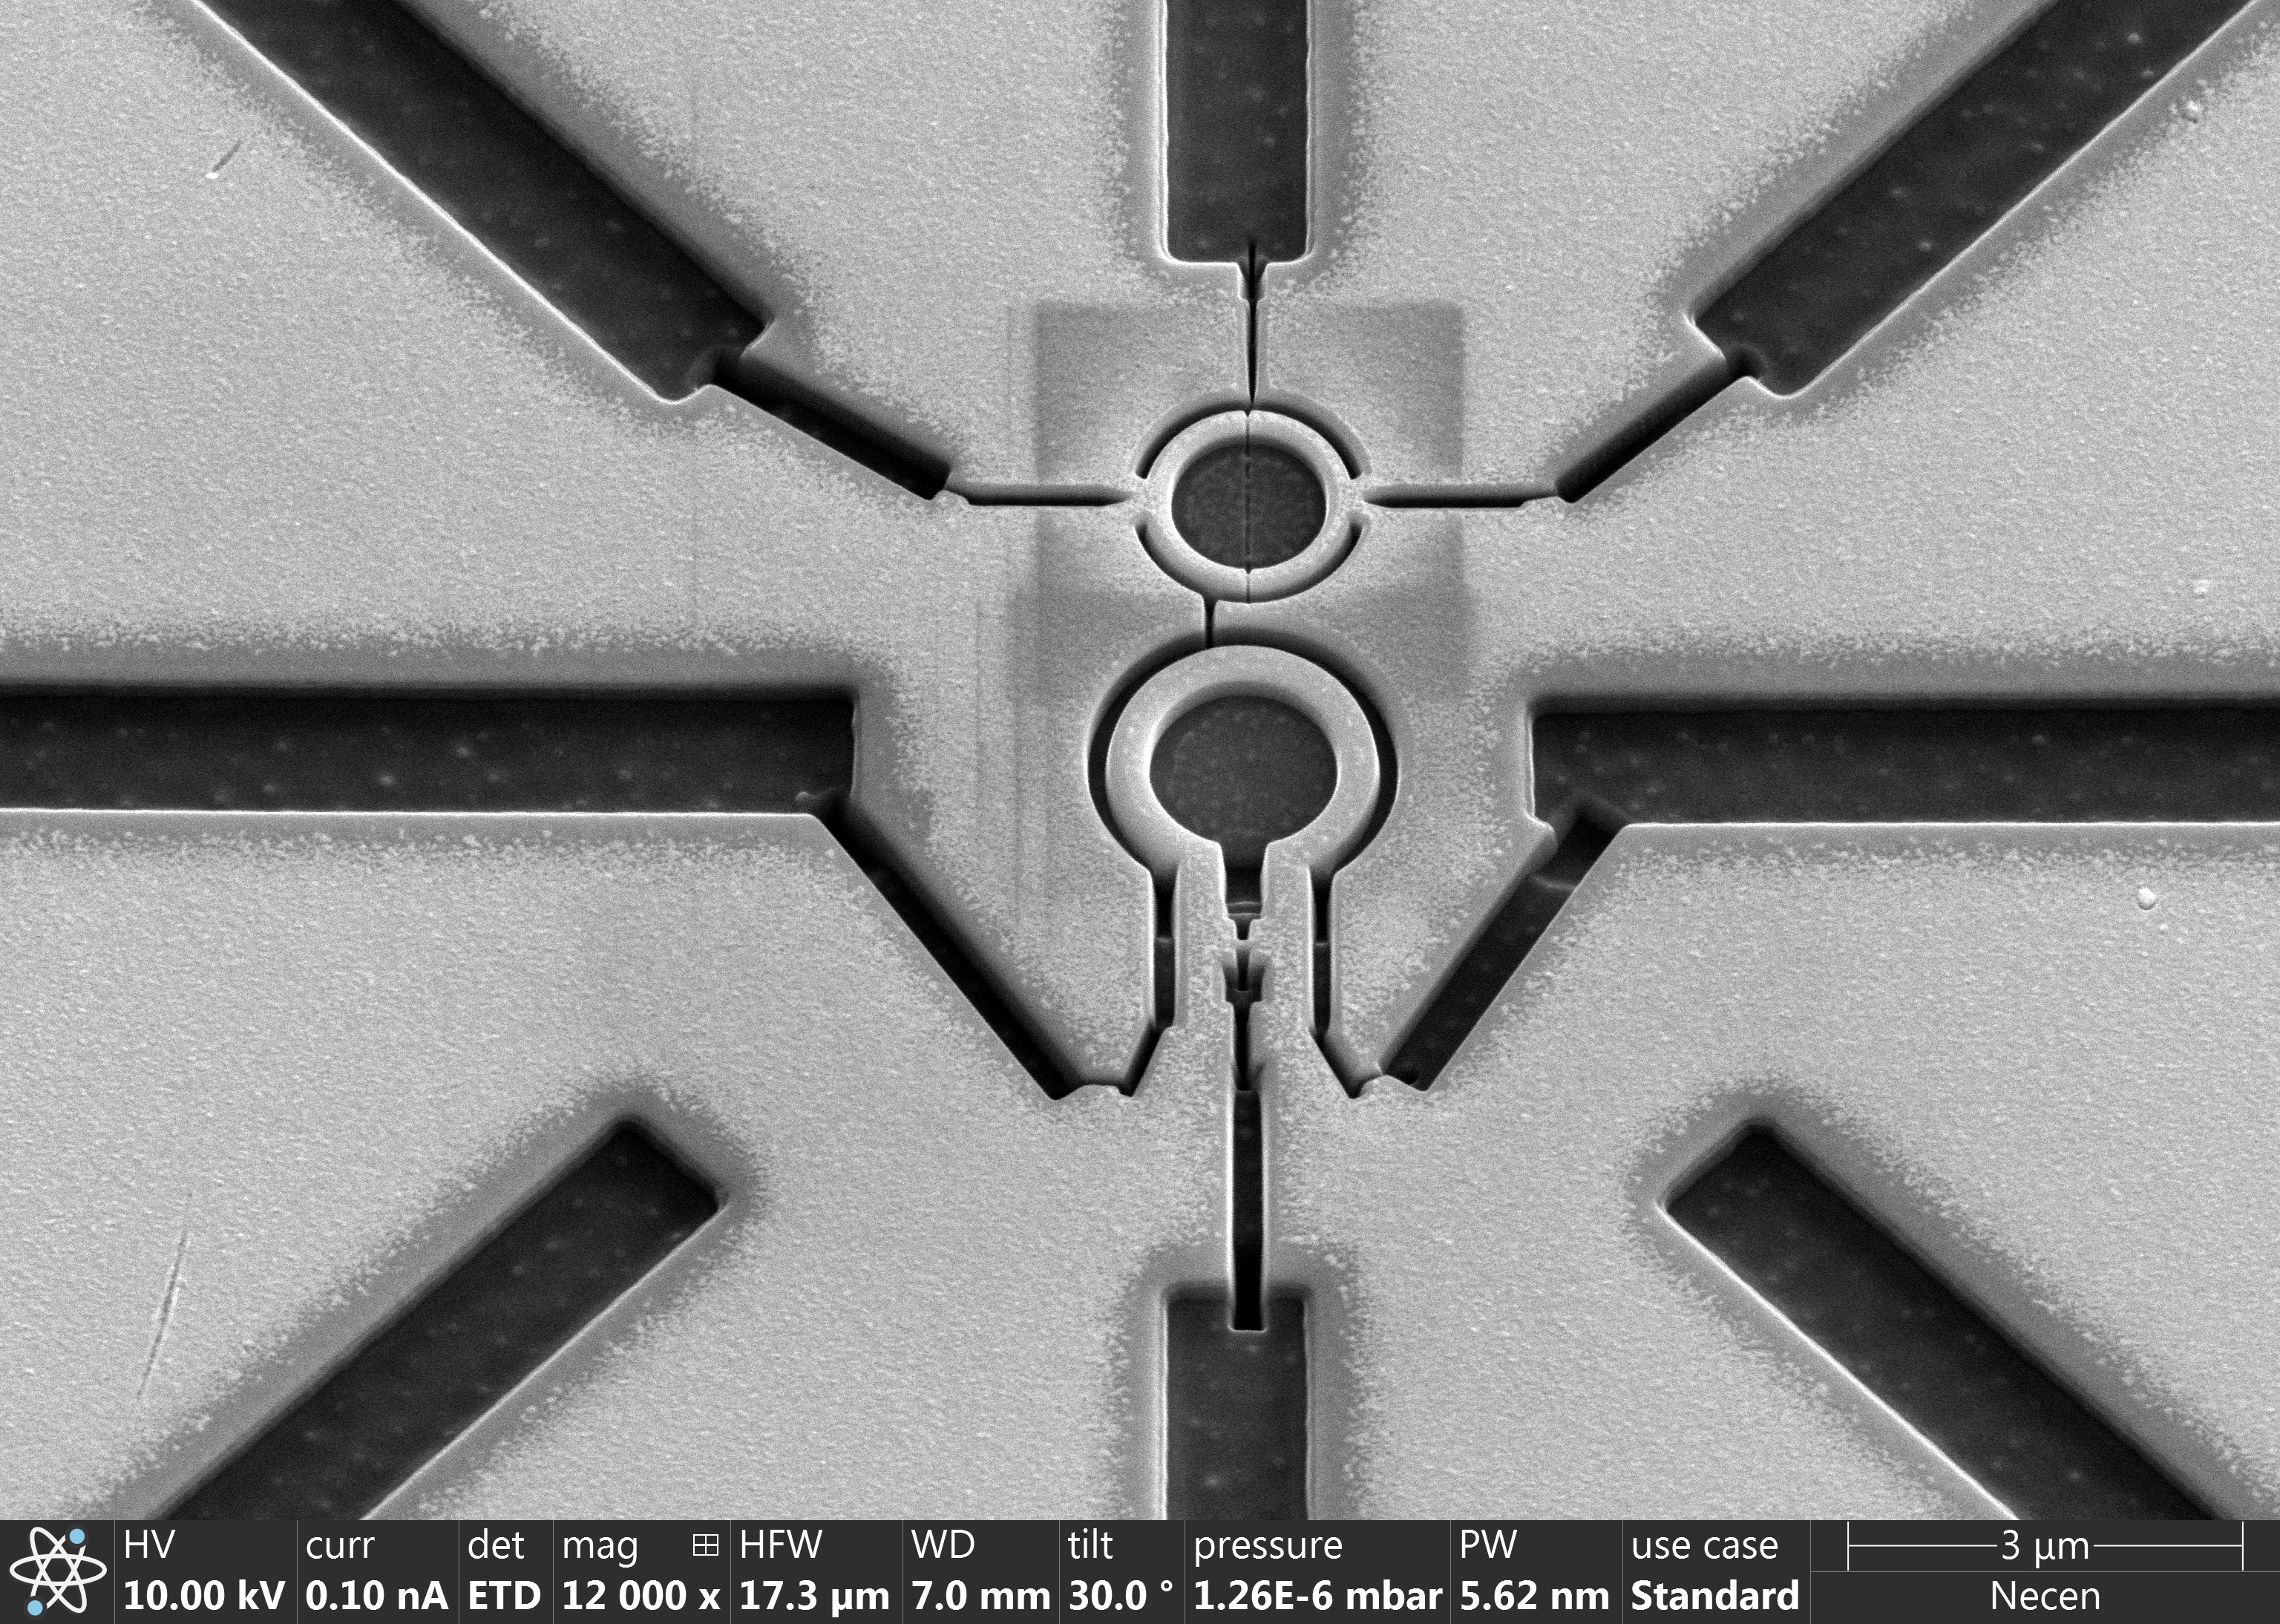
\includegraphics[width=\textwidth]{figures/samples/CP1/CP1.2H_SEM_overview.jpg}
		\subcaption{Overview of the fine structures. The thick leads go to \qty{300}{\micro\meter} by \qty{300}{\micro\meter} contact pads. On top we see the dc-SQUID and on the bottom the junction loop.}
	\end{subfigure}
	\hfill
	\begin{subfigure}[t]{0.3\textwidth}
		\centering
		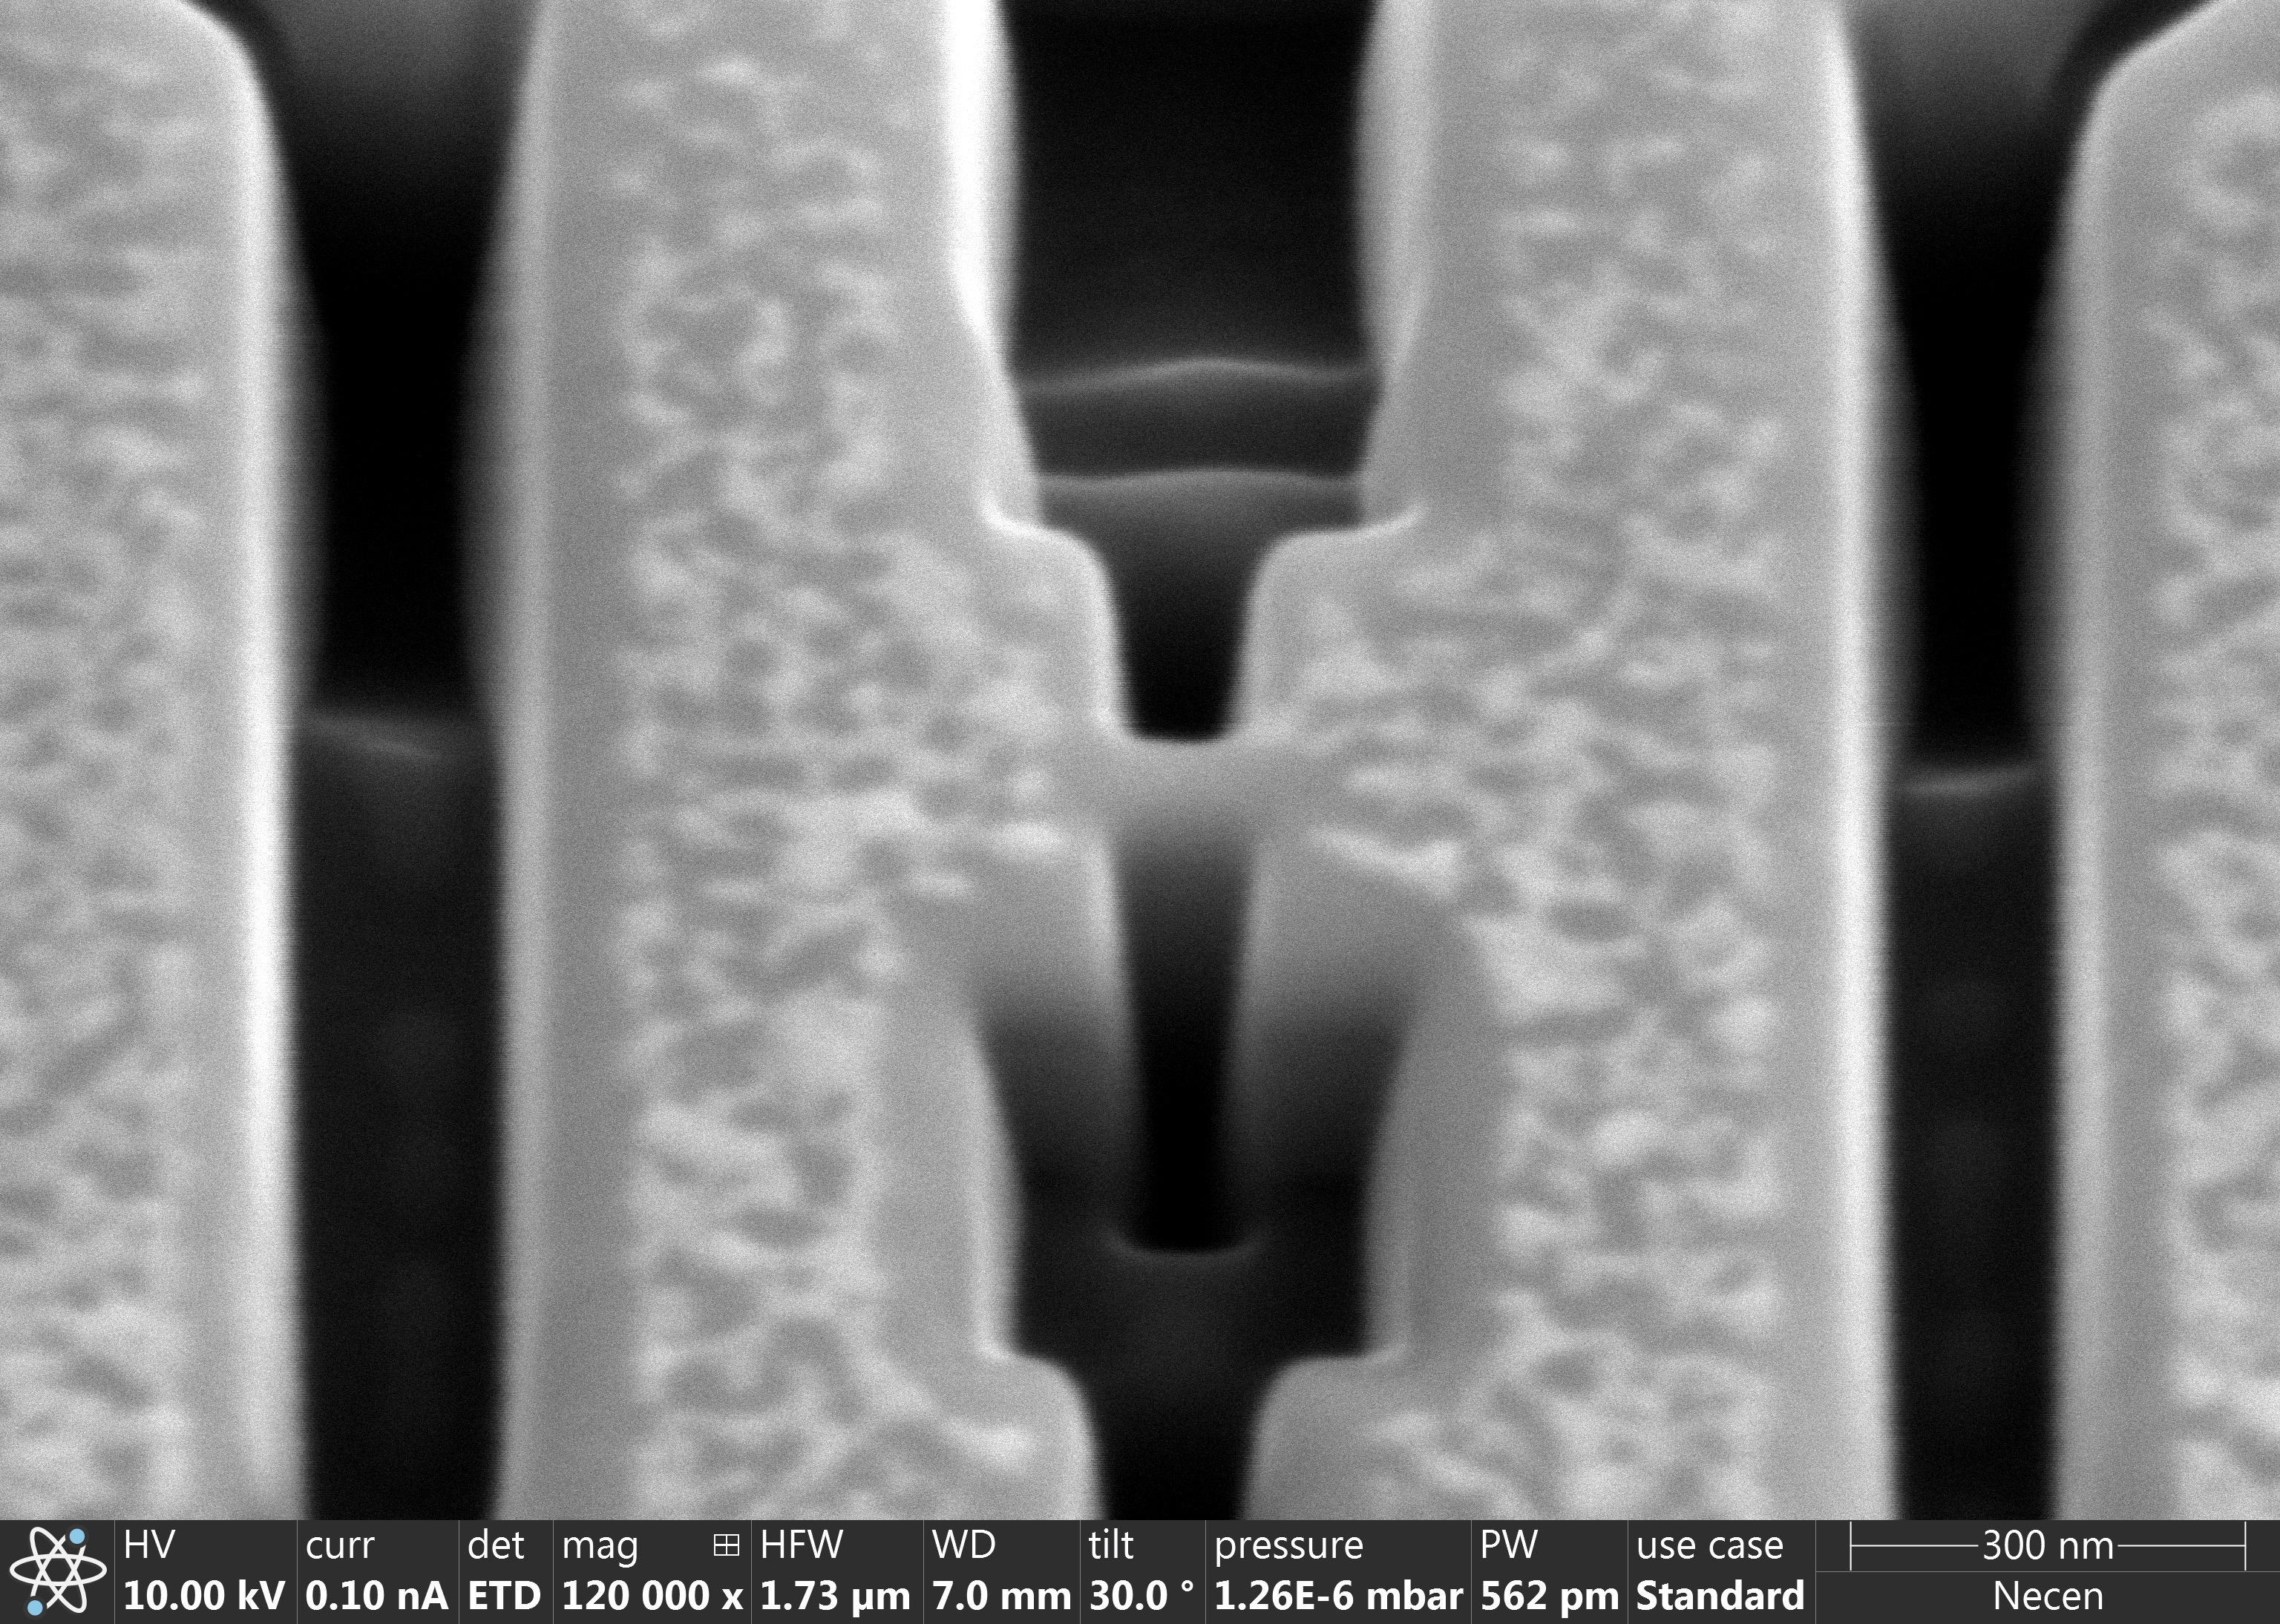
\includegraphics[width=\textwidth]{figures/samples/CP1/CP1.2H_SEM_junction.jpg}
		\subcaption{Zoomed in view of the junction, the size of the junction is \qty{100}{\nano\meter} by \qty{80}{\nano\meter}.}
	\end{subfigure}
	\hfill
	\begin{subfigure}[t]{0.3\textwidth}
		\centering
		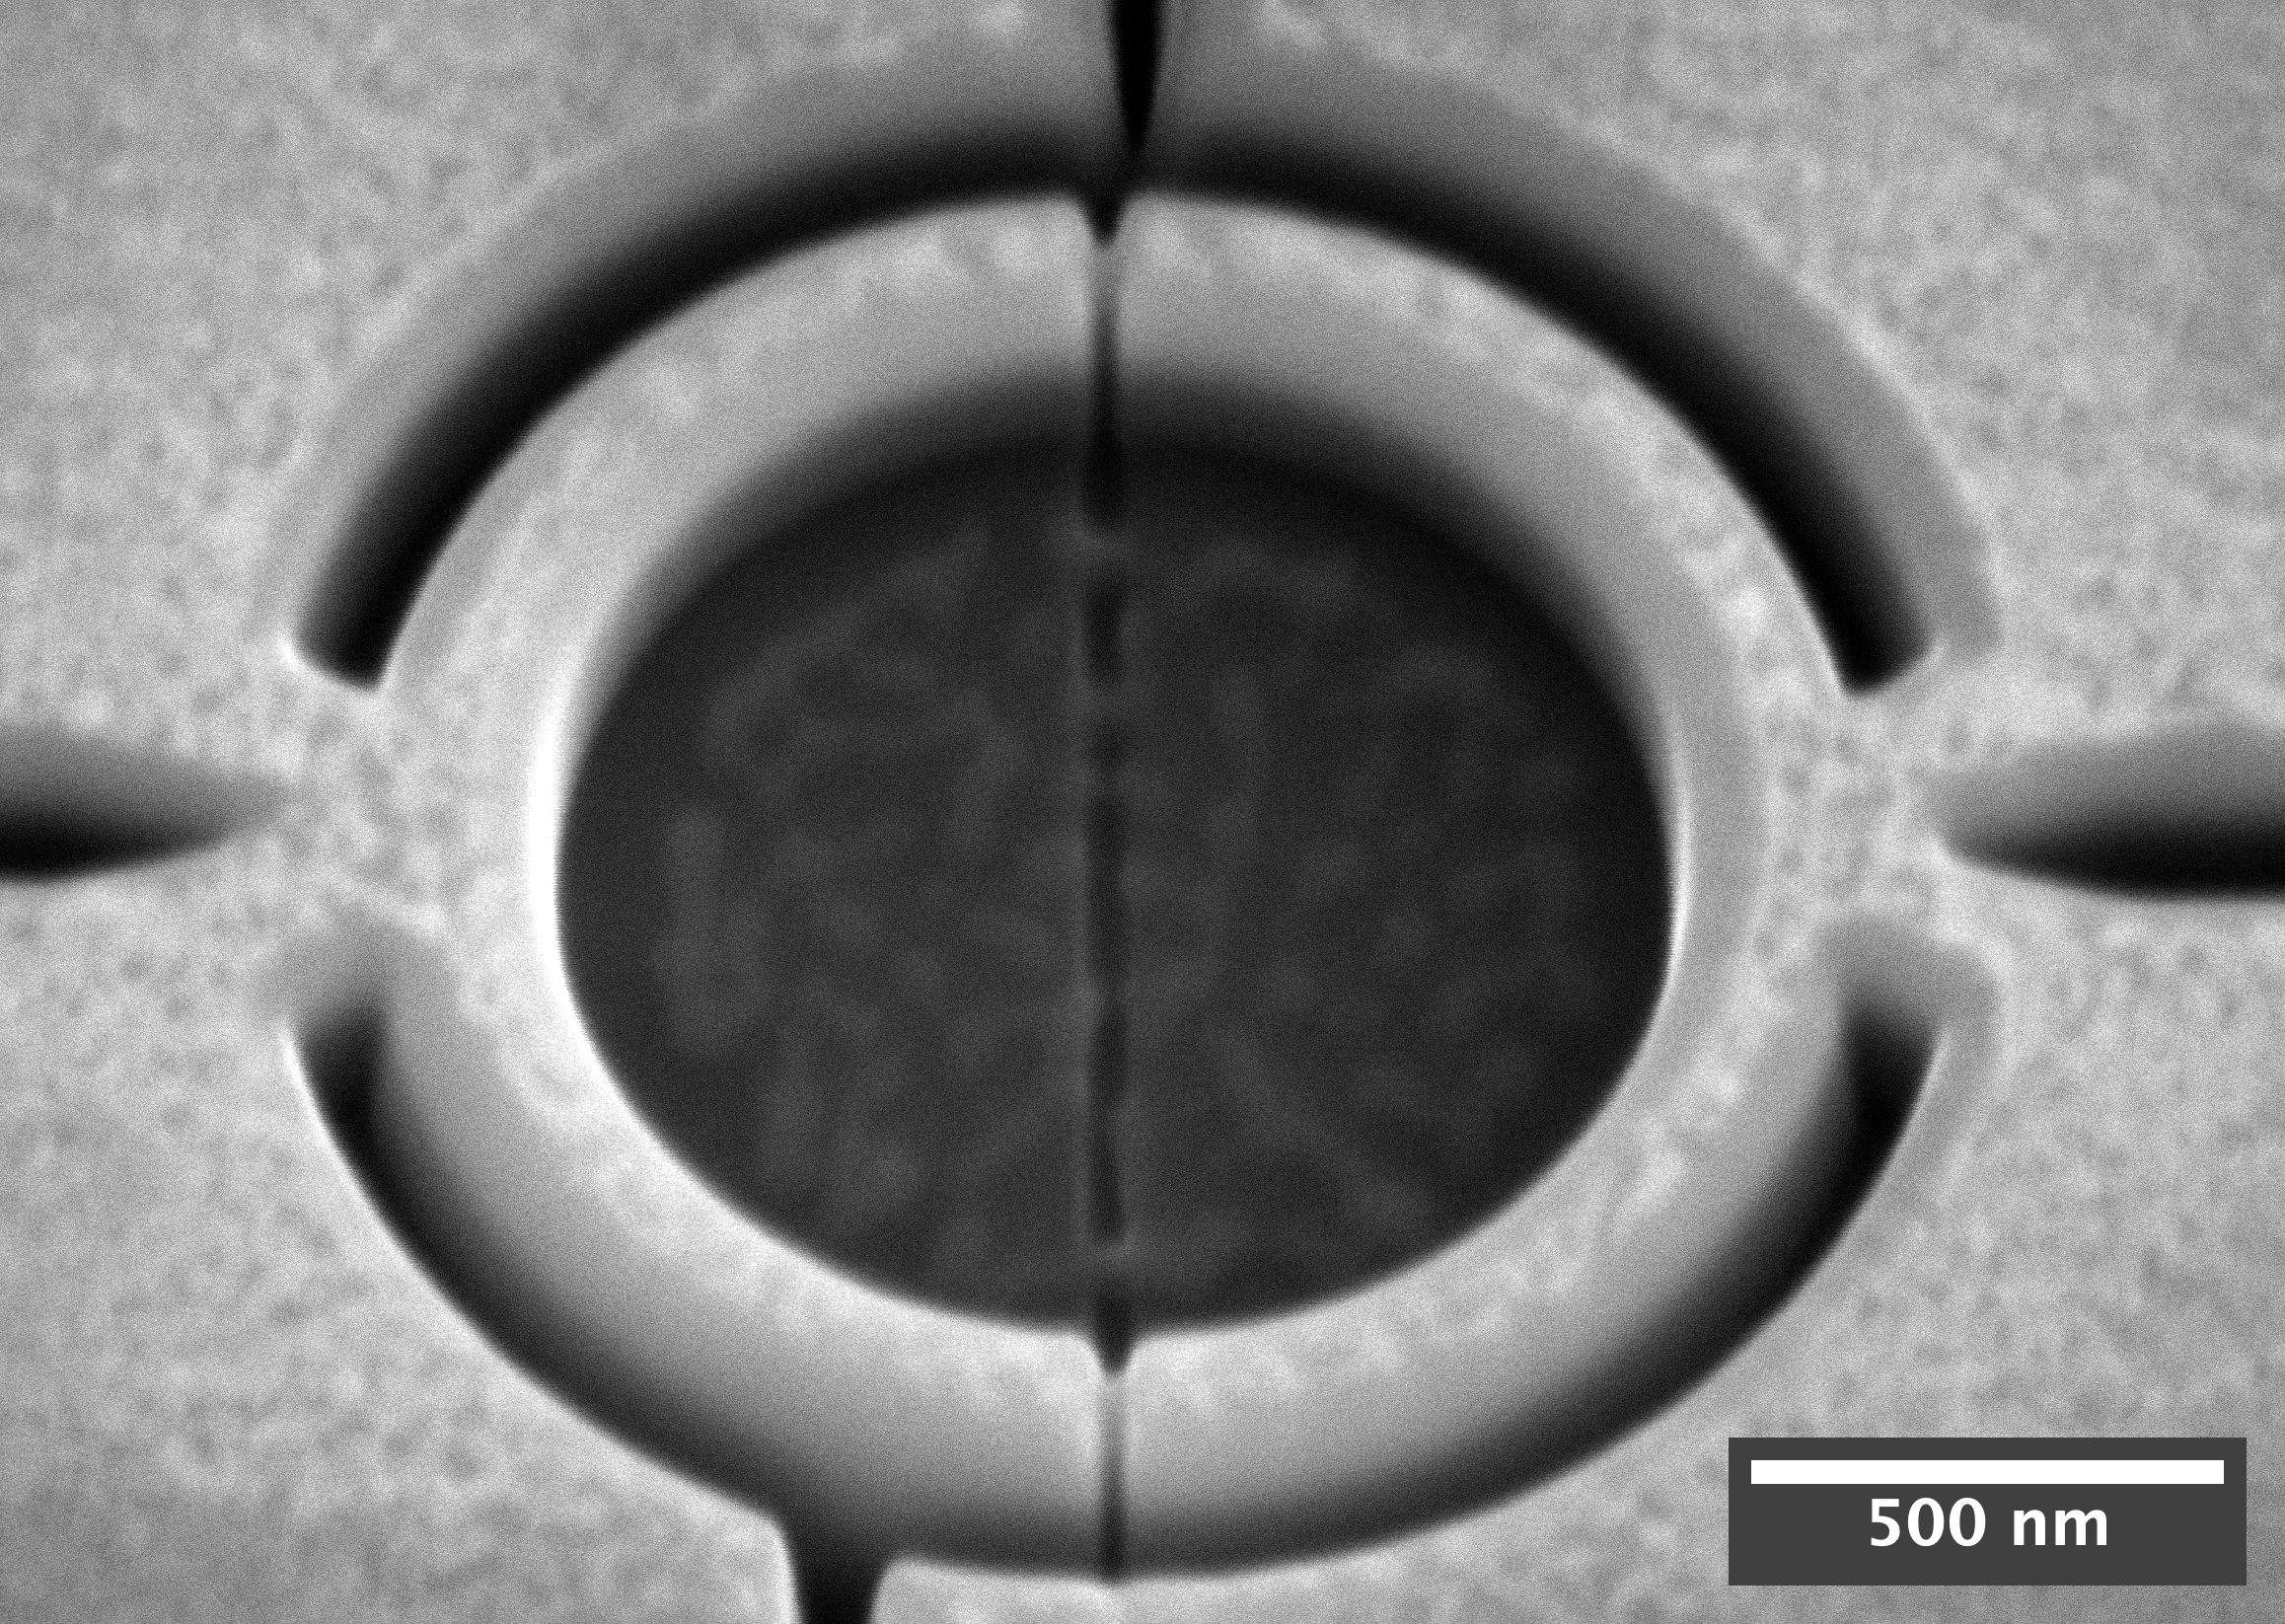
\includegraphics[width=\textwidth]{figures/samples/CP1/CP1.2H_SEM_SQUID.jpg}
		\subcaption{Zoomed in view of the dc-SQUID. The inner and outer diameters are \qty{1.195}{\micro\meter} and \qty{1.608}{\micro\meter} respectively. The width of the junction is \qty{19}{\nano\meter}.}
	\end{subfigure}

	\caption{Fine structures of sample CP1.2H after the FIB.}
	\label{fig:CP1.2H-SEM-images}
\end{figure}

\subsection{Results and discussion}
% !TEX root = ../../../thesis.tex
During the cool down of the Teslatron cryostat in which we measured the sample, we used a 4-point measurement to determine the resistance of the dc-SQUID. See Figure \ref{fig:CP1.1H-SQUID-RT}. We note that the sample becomes superconducting at \qty{8}{\kelvin} and has a quite sharp transition. This is above the expected transition temperature of \qty{7.5}{\kelvin} which was measured before on a thin film made from the same sputtering target. This might be explained however by the fact that the \ce{Nb} target had not been used in a while\footnote{It had last been used more than a year ago when the thin film was made.}. As such it is likely that when we sputtered the thin film that it had much more contaminations. $T_c$ for pure \ce{Nb} is \qty{9.2}{\kelvin}\cite{maxfieldSuperconductingPenetrationDepth1965}, since we use sputtering it is not surprising to find a lower $T_c$.

\begin{figure}[h]
	\centering
	\import{figures/samples/CP1}{CP1.2H_critical_temperature.pgf}
	\caption{Resistance over temperature between \qtyrange{2}{300}{\kelvin} for the dc-SQUID. The inset provides a detailed view of the superconducting transition.}
	\label{fig:CP1.1H-SQUID-RT}
\end{figure}

Additionally we determined the temperature dependence of the critical current, see Figure \ref{fig:CP1.1H-SQUID-critical-current-temperature-dependence}. We note that, similar to what we see in Figure \ref{fig:CP1.1H-SQUID-RT}, that there are two transitions. The obvious one is a very sharp transition but there is a second much more subtle transition. For example at \qty{7.6}{\kelvin} (inset of Figure \ref{fig:CP1.1H-SQUID-critical-current-temperature-dependence}) we note the sharp transition around \qty{170}{\micro\ampere} and the subtle transition near \qty{50}{\micro\ampere}. The sharp transition is for the bulk of the superconductor (leads, contact pads, etc.) whilst the more subtle one is from the dc-SQUID's junctions. This defines the range in which we should measure our dc-SQUID when using it as a magnetometer at certain temperatures.

\begin{figure}[h]
	\centering
	\import{figures/samples/CP1}{CP1.2H_critical_current.pgf}
	\caption{Temperature dependence of the critical current of the dc-SQUID. The left image shows voltage and its inset the IV-curve at \qty{7.6}{\kelvin}. The right image shows resistance, calculated by taking $dV/dI$. The plot uses linear interpolation.}
	\label{fig:CP1.1H-SQUID-critical-current-temperature-dependence}
\end{figure}

\begin{figure}[h]
	\centering
	\import{figures/samples/CP1}{CP1.2H_SQUID_B_field_sweep.pgf}
	\caption{}
\end{figure}

% \begin{figure}[h]
% 	\centering
% 	\import{figures/samples/CP1}{CP1.2H_voltage_drift.pgf}
% 	\caption{DC voltage measured by a shorted Keithley 2182A Nanovoltmeter. The RMS noise is \qty{15.90}{\nano\volt}, which is just above the \qty{15}{\nano\volt} as stated in the datasheet\cite{keithleyKeithley2182ANanovoltmeter}. The sampling rate was \qty{0.55\pm0.01}{\hertz}. The Fourier transform used to determine the PSD assumes a constant sampling rate.}
% \end{figure}

% Periodicity deviates most likely due to a malfunction of the Teslatron.

\section{Sample CP2.6B}
% !TEX root = ../../../thesis.tex
This sample's goal was to fix the shortcomings of our first sample. The first thing we want to improve is the dc-SQUID sensitivity. To do so SNS junctions were used instead of constriction junctions. SNS junctions were used in our group before and yielded good results.\cite{rogSQUIDontipMagneticMicroscopy2022} Furthermore, in order to decrease the chance of shorts we use a \ce{Si} with a thermal oxide on top. Additionally, to improve the coupling between the dc-SQUID and the junction loop we used a square geometry instead of a circular one. 

\subsection{Fabrication}
\label{sec:CP2.6B-fabrication}
% !TEX root = ../../../thesis.tex
%TODO: fix values.
In order to make SNS junctions we first sputtered \qty{1}{\nano\meter} of \ce{Cu} on our \ce{SiO} wafer, on top of this we added our \qty{1}{\nano\meter} of \ce{Nb} and capped it with \qty{7}{\nano\meter} of \ce{Au}. We again used the FIB to create the fine structures, see Figure~\ref{fig:CP2.6B-SEM-images}.

\begin{figure}[ht]
	\begin{subfigure}[t]{0.3\textwidth}
		\centering
		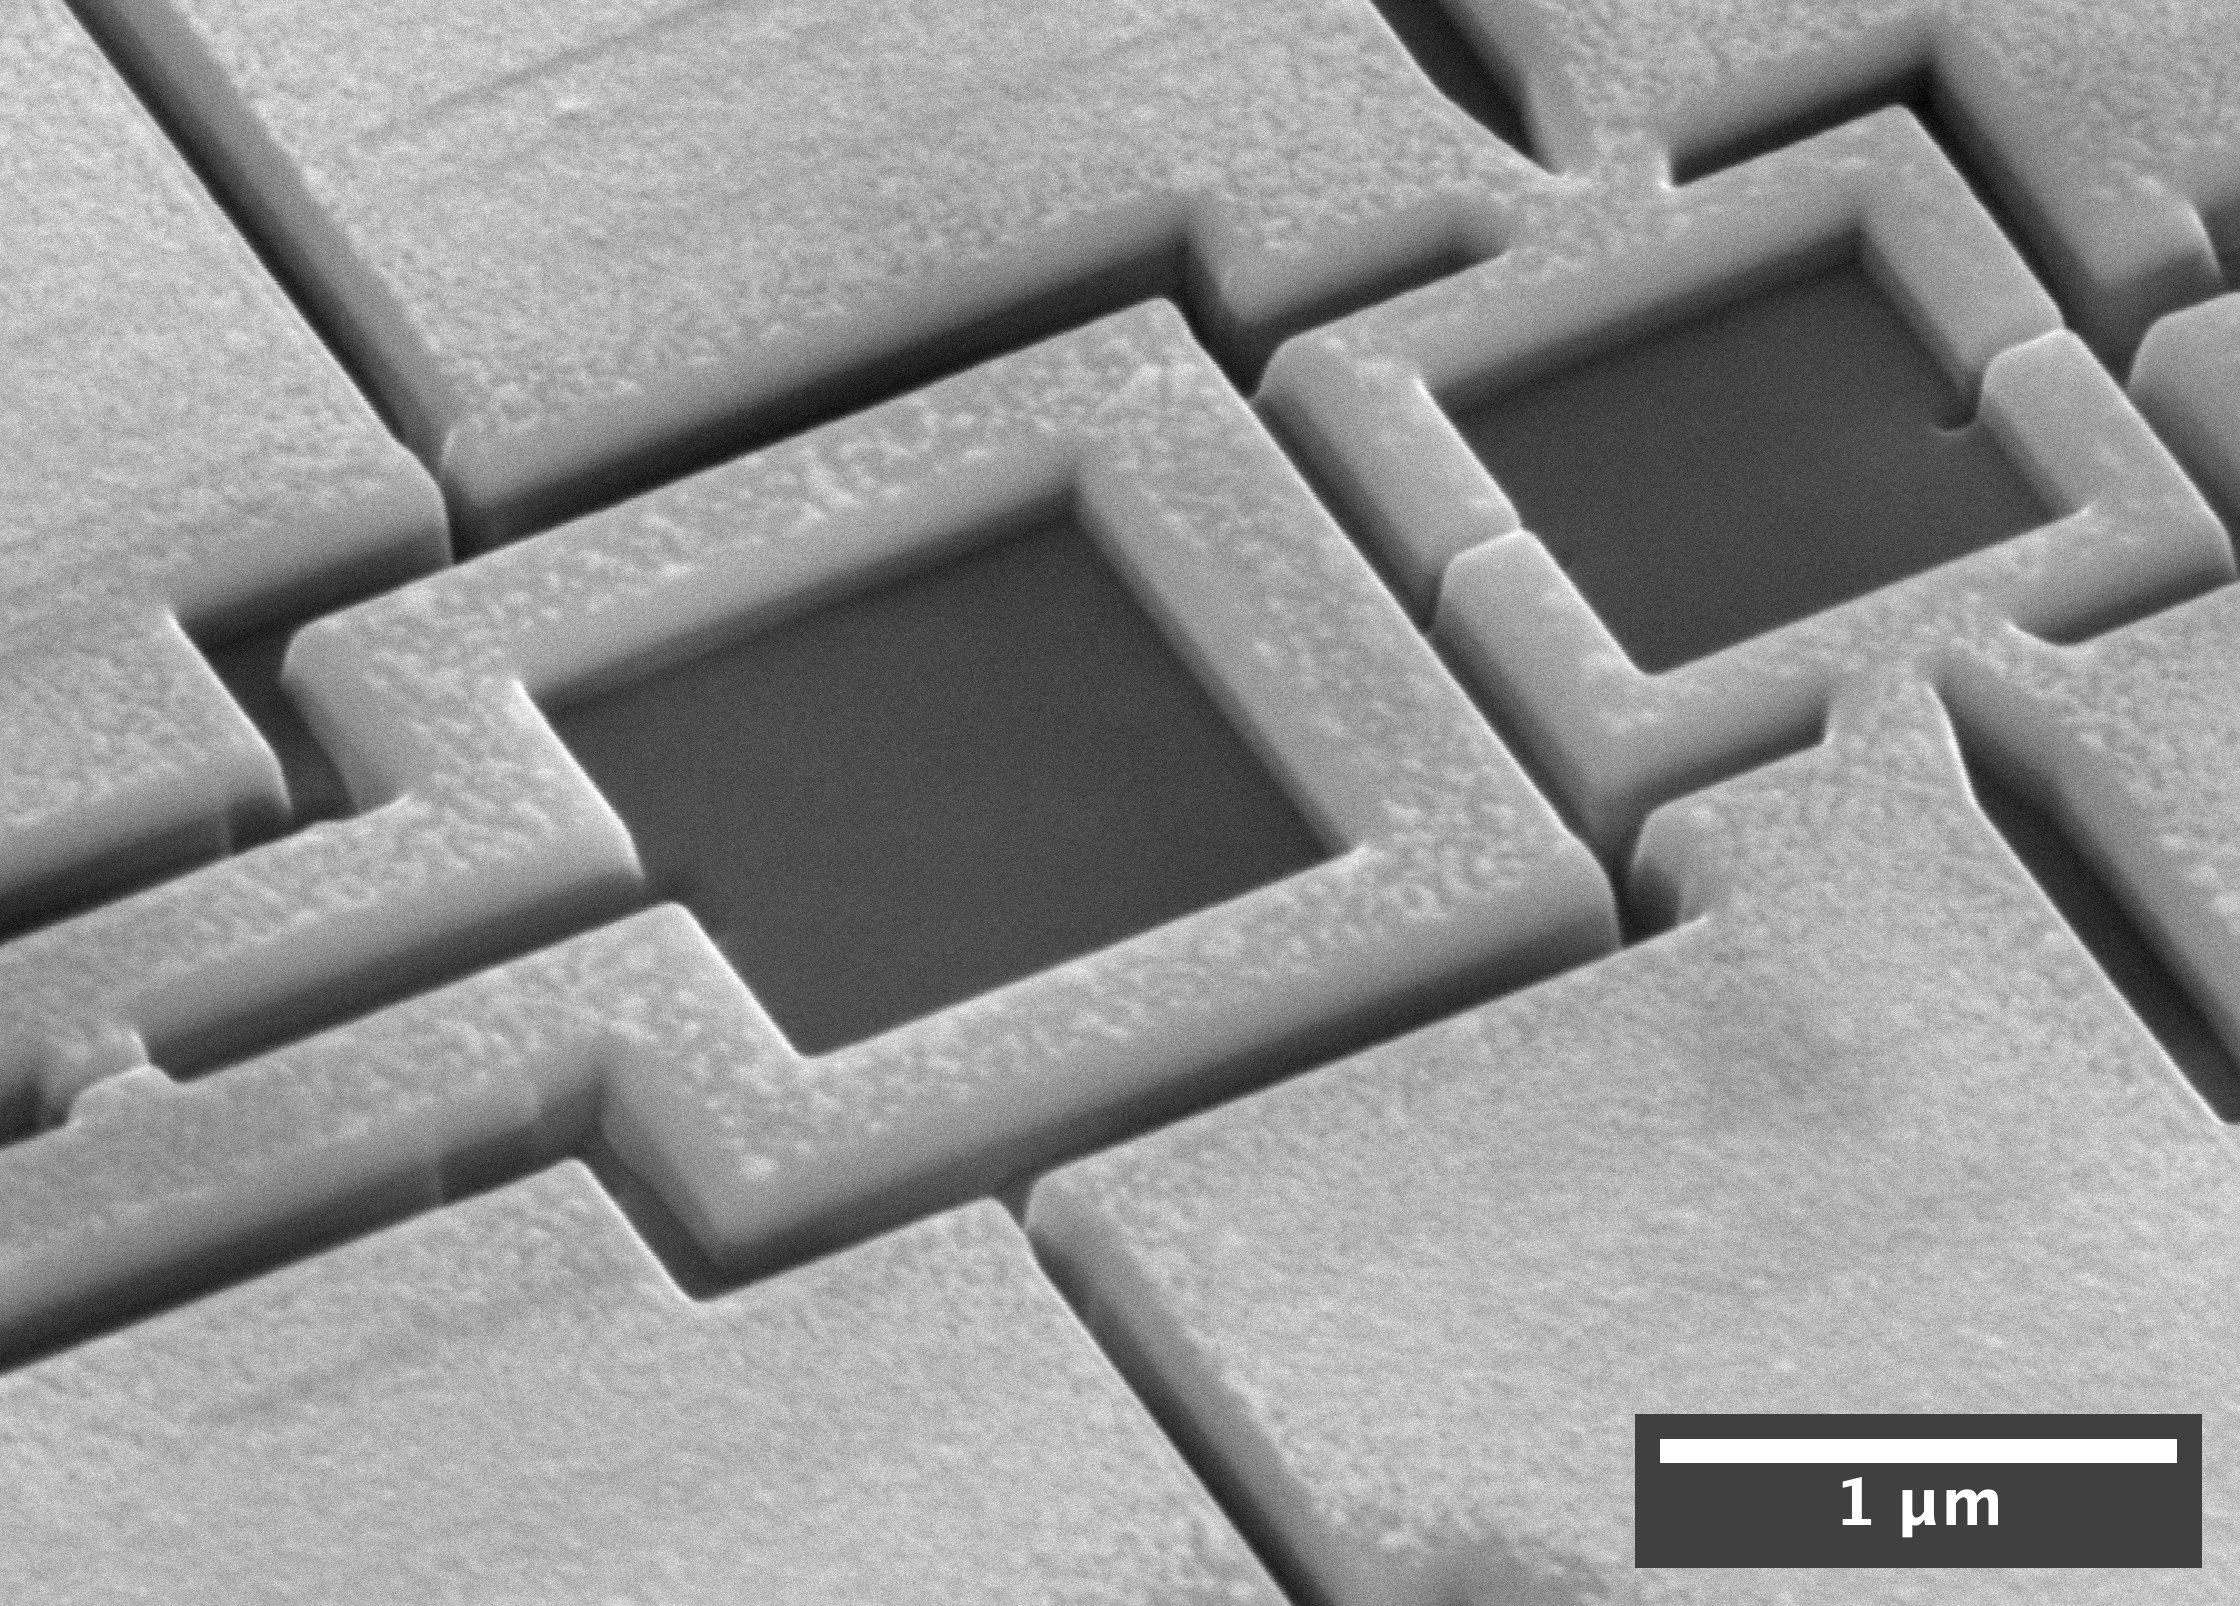
\includegraphics[width=\textwidth]{figures/samples/CP2/CP2.6B_SEM_overview.jpg}
		\subcaption{Overview of the device. The top loop shows the dc-SQUID and the bottom is the junction loop.}
	\end{subfigure}
	\hfill
	\begin{subfigure}[t]{0.3\textwidth}
		\centering
		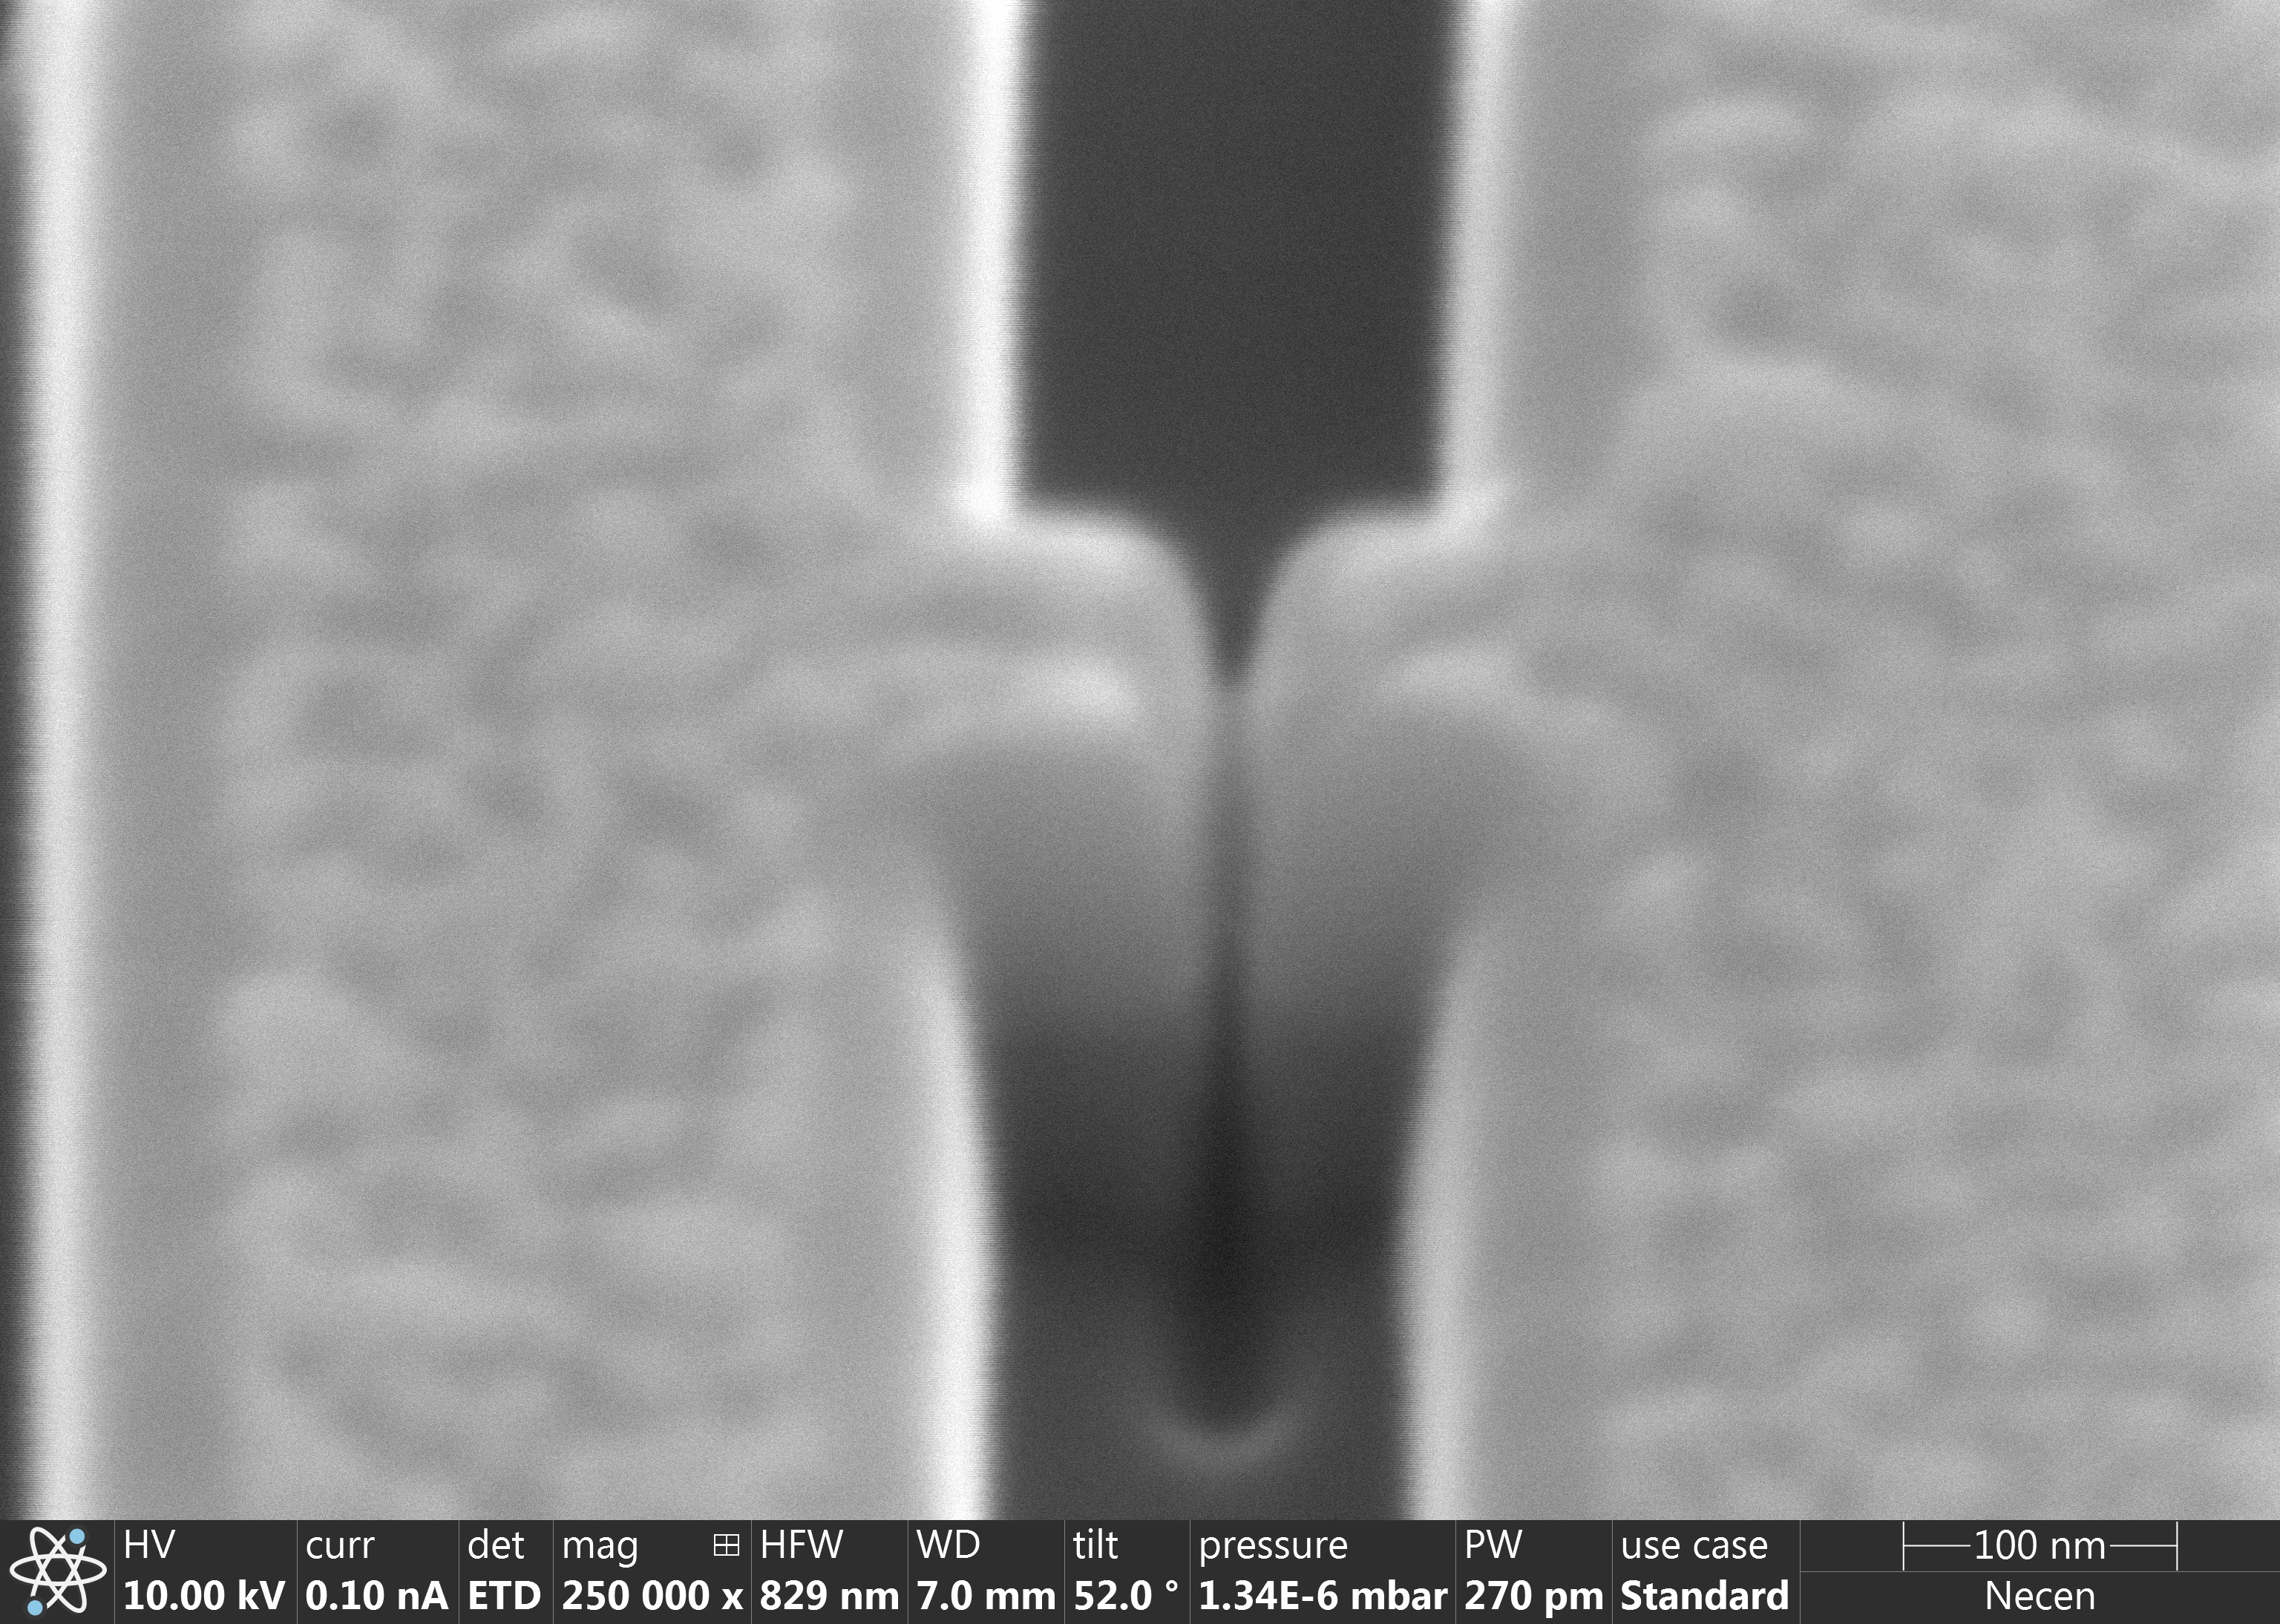
\includegraphics[width=\textwidth]{figures/samples/CP2/CP2.6B_SEM_junction.jpg}
		\subcaption{Zoomed in view of the junction, the width of the junction is \qty{12}{\nano\meter}.}
	\end{subfigure}
	\hfill
	\begin{subfigure}[t]{0.3\textwidth}
		\centering
		\includegraphics[width=\textwidth]{figures/samples/CP2/CP2.6B_SEM_SQUID.jpg}
		\subcaption{Zoomed in view of the dc-SQUID. The width of the junctions is \qty{22}{\nano\meter}.}
	\end{subfigure}

	\caption{Fine structures of sample CP2.6B after the FIB. See Table~\ref{tab:CP2.6B-geometries} for the exact geometries of the sample.}
	\label{fig:CP2.6B-SEM-images}
\end{figure}

\begin{table}
	\begin{subtable}{.5\linewidth}
		\centering
		\begin{tabular}{@{}lrr@{}}
			\toprule
			Parameter & Value \\ \midrule
			Junction loop $\diameter_{\text{outer}}$ & \qty{1.9}{\micro\meter} \\
			Junction loop $\diameter_{\text{inner}}$ & \qty{1.2}{\micro\meter} \\
			dc-SQUID $\diameter_{\text{outer}}$ & \qty{1.6}{\micro\meter} \\
			dc-SQUID $\diameter_{\text{inner}}$ & \qty{1.1}{\micro\meter} \\
			spacing & \qty{0.1}{\micro\meter} \\
			$d_{\ce{Cu}}$ & \qty{25}{\nano\meter} \\
			$d_{\ce{Nb}}$ & \qty{70}{\nano\meter} \\
			$d_{\ce{Au}}$ & \qty{7}{\nano\meter} \\
			\bottomrule
		\end{tabular}
    \end{subtable}
    \begin{subtable}{.5\linewidth}
    	\centering
    	\begin{tabular}{@{}lrr@{}}
    		\toprule
    		Parameter & Value \\ \midrule
    		$L_{l}$ & \qty{3.0}{\pico\henry} \\
			$L_{s}$ & \qty{3.0}{\pico\henry} \\
			$M$ & \qty{-0.2}{\pico\henry} \\
			$\delta$ & \num{0.001} \\
			$\kappa$ & \num{-0.058} \\
    		\bottomrule
    	\end{tabular}
    \end{subtable}
    \caption{The \textbf{left} table provides an overview of the geometries of CP2.6B as determined by SEM imaging and sputtering rates. The \textbf{right} table gives an overview of parameters found using a simulation based on the geometries. The geometries are based on sample CP1.2H.}
    \label{tab:CP2.6B-geometries}
\end{table}

\subsection{Results and discussion}
% !TEX root = ../../../thesis.tex
Figure~\ref{fig:CP2.6B_RT_curves} shows the RT-curves for the junction loop and dc-SQUID. The critical temperature for the bulk of the sample is lower (\qty{7}{\kelvin}) compared to the first sample (\qty{8}{\kelvin}). This can be explained by the proximity effect due to the interface between the \ce{Cu} and \ce{Nb}.\cite{cirilloSuperconductingProximityEffect2005} The longer `tail' is characteristic for SNS junctions as the normal metal slowly proximises.

\begin{figure}[ht!]
	\centering
	\input{figures/samples/CP2/CP2.6B_RT_curves.pgf}
	\caption{Temperature dependences of the 4-point resistance measured over the dc-SQUID and the junction loop. We note that just before the superconducting transition that there is a small bump in resistance of the dc-SQUID and a long `tail' before reaching \qty{0}{\ohm}. Compared to this the transition of the junction loop is much sharper.}
	\label{fig:CP2.6B_RT_curves}
\end{figure}

Figure~\ref{fig:CP2.6B_SQUID_calibration_curves} shows the interference pattern of the dc-SQUID for several bias currents. The periodicity in the the data is roughly \qty{1}{\milli\tesla}. This matches the expected period. Furthermore, the sensitivity in the linear regime increased by a factor 3 compared to the previous sample. The comparison is a bit unfair as the bias current is also 3 times larger. In the previous sample however, such a large bias current was simply not possible. There are two issues with this result. First off, the period of the pattern does not seem to be constant. Secondly, the offset (in the field axis) varies a lot between curves whilst they should all be zero. Both these issues can be explained by vortices getting trapped in the magnet or sample. 

\begin{figure}[ht!]
	\centering
	\input{figures/samples/CP2/CP2.6B_SQUID_constant_bias_calibration_curves.pgf}
	\caption{Voltage measured over the dc-SQUID for various bias currents over external magnetic field. The patterns have been fitted to a sinusoid and the slanted lines illustrate the linear response. The sensitivities in the linear regions are \qtylist{160;232;279;346}{\micro\volt/\milli\tesla} respectively. For \qty{380}{\micro\ampere} the curve has been measured twice (annotated with a \dag).}
	\label{fig:CP2.6B_SQUID_calibration_curves}
\end{figure}

During an attempt to measure the CPR, the IV-curves showed anomalous spikes. Initially we attributed this to vortex trapping. However, upon closer inspection these jumps are highly correlated with the actual magnetic field produced by the magnet. Figure~\ref{fig:CP2.6B_PPMS_magnetic_field_drift} shows a clear correlation between the dc-SQUID voltage and the magnetic field as measured by the magnet. Even though a constant setpoint of \qty{0}{\milli\tesla} was used, there is quite some drift. This is because the magnet does not have a persistent mode but instead uses a feedback loop. This feedback loop has a dead band of \qty{50}{\micro\tesla}. Changing the setpoint of the field or the rate of change did not have a significant effect.

\begin{figure}[ht!]
	\centering
	\input{figures/samples/CP2/CP2.6B_PPMS_magnetic_field_drift_0mT_rate_200uT.pgf}
	\caption{Correlation between the actual magnetic field of the cryostat and the voltage measured over the dc-SQUID. The setpoint of the magnetic field is \qty{0}{\milli\tesla} and a change rate of \qty{200}{\micro\tesla\per\second}. The standard deviation from the setpoint is \qty{30}{\micro\tesla}.}
	\label{fig:CP2.6B_PPMS_magnetic_field_drift}
\end{figure}

In an attempt to fix the `noise' caused by the feedback loop, the magnet was turned off. Unfortunately, it never turned back on as the magnet controller was broken. A downside of this, is that it was no longer possible to read out the value of the field. An attempt was made to measure the CPR again by using a constant bias current of \qty{380}{\micro\ampere} for the dc-SQUID. It should be mentioned that during these measurements there appeared to be a lot of drift causing measurements to differ widely. An external magnetic field was likely responsible for this. Possibly this was still caused by the magnet controller as, later on when it was replaced, this did not seem to be an issue anymore.

Figure~\ref{fig:CP2.6B_SQUID_voltage_over_total_current} shows the raw data from one of the CPR measurements. There is a clear periodicity in the signal of around \qty{200}{\micro\ampere} and a somewhat linear trend on top of that. This specific measurement is presented because it has no unexpected jumps in the dc-SQUID voltage; has a sufficiently small sample spacing; covers a wide enough range to see several periods; and measured both positive and negative currents. Using different sample spacings did not affect the measured periodicity.

\begin{figure}[ht!]
	\centering
	\input{figures/samples/CP2/CP2.6B_SQUID_voltage_over_total_current.pgf}
	\caption{The voltage over the dc-SQUID over the applied total current. A bias current through the dc-SQUID of \qty{380}{\micro\ampere} was used, the measurement was done at \qty{3}{\kelvin}.}
	\label{fig:CP2.6B_SQUID_voltage_over_total_current}
\end{figure}

Using the second calibration curve for \qty{380}{\micro\ampere} bias current we converted the dc-SQUID voltage to a flux. A linear fit is used to determine the mutual inductance to be $\qty{-0.339\pm0.005}{\pico\henry}$. This is almost twice as large as the simulated value in Table~\ref{tab:CP2.6B-geometries}. Similarly, by exploiting the $\Phi_0$-periodicity of the CPR, the junction's loop's inductance was found to be \qty{6\pm1}{\pico\henry}. Again this is almost twice the as large as the simulated value in Table~\ref{tab:CP2.6B-geometries}. Using the proportionality between $\Phi_l$ and $\gamma$ the flux was converted to a phase. Figure~\ref{fig:CP2.6B_super_current_over_phase} shows the result of this analysis.

\begin{figure}[ht!]
	\centering
	\input{figures/samples/CP2/CP2.6B_super_current_over_phase.pgf}
	\caption{Supper current through the junction loop over junction loop flux. See main text for details on how this result was obtained. The dashed line is to improve visual clarity.}
	\label{fig:CP2.6B_super_current_over_phase}
\end{figure}

The amplitude of the oscillations is around \qty{60}{\micro\ampere} and the pattern contains quite steep slopes. Furthermore, the pattern `dips' down a bit and does not oscillate around the same mean. Most likely this is because the dc-SQUID is not biased in its linear regime and thus a measurement artefact.

It is clear that two major issues with this result are the lack of resolution and the calibration. Future measurements should take much smaller steps. Furthermore, because it was not possible to keep the dc-SQUID in the linear response region the sensitivity and calibration were suboptimal. 
	% !TEX root = ../../thesis.tex
\chapter{Conclusion}
In this thesis a method to measure the current-phase relation of a Josephson junction was developed and its performance demonstrated. Our method utilises a dc-SQUID inductively coupled to a superconducting loop with a single junction. By passing a current through the junction's loop it is possible to modulate the phase of the junction. This phase is proportional to the flux in the loop which is measured by the dc-SQUID. From the total current and the measured flux the current-phase relation can be extracted.

The temperature dependence of the current-phase relation of a SNS junction was qualitatively determined using the above method. Starting from \qtyrange{2.8}{3.6}{\kelvin} the $2\pi$-periodic current-phase relation becomes more sinusoidal as the critical temperature is approached. Furthermore between \qtyrange{2.8}{3.4}{\kelvin} we determined the critical current to decrease from \qtyrange{90}{45}{\micro\ampere}. Both these observations are in line with theoretical models. However, the data does not yet allow us to distinguish between diffusive and ballistic behaviour.

Whilst successful, further improvements are possible. Most notably the implementation of a flux-locked loop. This will allow biasing the dc-SQUID at its working point. This means that the measurements will become more sensitive. Furthermore, a flux-locked loop allows integrating the results over a longer period improving the accuracy. An attempt was made to implement the flux-locked loop using a current modulation line. However, that sample was unfortunately destroyed. Future projects can use its design.

\section{Outlook}
The potential of the method has been demonstrated. Future research should improve the method. The most promising improvement is the addition of a flux-locked loop dc-SQUID readout scheme that improves the sensitivity and decreases unwanted background interference.  In order to measure the current-phase relation of \ce{Sr2RuO4} minor adjustments to the method are needed. It is impractical to make both the junction's loop and the dc-SQUID from the same crystal. But we can use our electron-beam-induced deposition facilities to directly deposit superconducting \ce{WC} next to the junction under study. Furthermore, we currently lack the knowledge on how to pin a single chiral domain wall. As such it is difficult to study a single chiral domain wall. Alternatively, it might be possible to incorporate a ring of \ce{Sr2RuO4} with two chiral domain walls instead of a single junction. In that case no additional weak links must be formed, or their behaviour negligible compared to the \ce{Sr2RuO4} ring.

	\appendix
	\chapter{Derivations}
	% !TEX root = ../../thesis.tex
\section{Phase-flux relation}
\label{app:derivation-phase-flux-relation}
We can write the magnetic field $\vec{B}$ as the curl of the magnetic vector potential $\vec{A}$. This allows us to rewrite the magnetic flux through the superconducting loop containing our junction in terms $\vec{A}$.
\begin{align}
	\Phi = \oiint \vec{B} \cdot d\vec{a} = \oiint \left(\nabla \times \vec{A}\right) \cdot d\vec{a} = \oint \vec{A} \cdot d\vec{l}
\end{align}
The closed integral over $\vec{A}$ can be any path enclosing the hole in the superconductor. It consists of two pieces, namely the junction and the rest of the loop.
\begin{align}
	\Phi = \int_{\text{JJ}} \vec{A} \cdot d\vec{l} + \int_{\text{loop}} \vec{A} \cdot d\vec{l}
	\label{eqn:magnetic-potential-integral}
\end{align}
For the integral over the junction we will use make use of the gauge-invariant phase (see Eq. \ref{eqn:gauge-invariant-phase}).
\begin{align}
	\gamma = \Delta\varphi_{\text{JJ}} - \frac{2\pi}{\Phi_0}\int_{\text{JJ}}\vec{A} \cdot d\vec{l} \Rightarrow \int_{\text{JJ}}\vec{A} \cdot d\vec{l} = \frac{\Phi_0}{2\pi} \left(\Delta\varphi_{\text{JJ}} - \gamma\right)
\end{align}
For the integral over the rest of the loop we will make use of the superfluid velocity\footnote{See \citetitle{tinkhamIntroductionSuperconductivity} equation 4.9, the equation has been converted to SI units.}:
\begin{equation}
	m^*\vec{v} = 2m_e\vec{v} = \hbar \nabla \varphi - \frac{e^*\vec{A}}{c} \stackrel{\text{SI}}{=} \hbar \nabla \varphi + 2e\vec{A}
	\label{eqn:superfluid-velocity}
\end{equation}
It allows us to rewrite:
\begin{align}
	\vec{A} = \frac{1}{2e}\left(\hbar \nabla \varphi_{\text{loop}} - 2m_e\vec{v}\right)
\end{align}
We can substitute $\vec{v}$ with a more useable expression in terms of the current density $\vec{J}$ and $\lambda$ using Eq. \ref{eqn:london-penetration-depth}.
\begin{align}
	\vec{J} = -2e|\psi|^2\vec{v} = -\frac{m_e}{\lambda^2e\mu_0}\vec{v} \Rightarrow \vec{v} = -\frac{\lambda^2e\mu_0}{m_e}\vec{J}
\end{align}
Combining the two equations gives us a useable expression for $\vec{A}$ in the loop:
\begin{align}
	\vec{A} &= \frac{1}{2e}\left(\hbar \nabla \varphi_{\text{loop}} + 2\lambda^2e\mu_0\vec{J} \right) \nonumber \\
	&= \frac{\Phi_0}{2\pi} \nabla \varphi_{\text{loop}} + \lambda^2\mu_0\vec{J}
\end{align}
We can now go back to Eq. \ref{eqn:magnetic-potential-integral}:
\begin{align}
	\Phi &= \underbrace{\frac{\Phi_0}{2\pi} \left(\gamma - \Delta\varphi_{\text{JJ}}\right)}_{\int_{\text{JJ}}\vec{A} \cdot d\vec{l}} \underbrace{- \frac{\Phi_0}{2\pi}\Delta \varphi_{\text{loop}} - \lambda^2\mu_0 \int \vec{J}\cdot d \vec{l}}_{\int_{\text{loop}}\vec{A}\cdot d\vec{l}} \nonumber \\
	&= \frac{\Phi_0}{2\pi} \left(\gamma - \underbrace{\left(\Delta\varphi_{\text{JJ}} + \Delta\varphi_{\text{loop}}\right)}_{\text{Multiple of } 2\pi} \right) - \lambda^2\mu_0 \int \vec{J}\cdot d \vec{l}
\end{align}
The phase must wind by a multiple of $2\pi$ to make sure that the wave function is uniquely defined at each point. Using this fact and the quantization of $\Phi$ in units of $\Phi_0$ we find:
\begin{align}
	\Phi &= \left(\frac{\Phi_0}{2\pi}\gamma - \lambda^2\mu_0 \int \vec{J}\cdot d \vec{l} \right) \mod \Phi_0 \\ 
	% \Rightarrow \gamma &= -\left(\frac{2\pi\Phi}{\Phi_0} + \frac{2\pi\lambda^2\mu_0}{\Phi_0} \int \vec{J}\cdot d \vec{l} \right) \mod 2\pi \\
	\gamma &= \frac{2\pi}{\Phi_0}\left(\Phi + \lambda^2\mu_0 \int \vec{J}\cdot d \vec{l} \right)
\end{align}

\section{Geometric factor $\tilde{j}$}
\label{app:derivation-geometric-factor-j}
The goal of this appendix section is to derive how to calculate $\tilde{j}$. In a rectangular thin film superconductor with thickness (height) $d$ on the order of $\lambda$ and width $w > \lambda$ such that $wd \gg \lambda$ then the current density a distance $x$ from the centre is given by\cite{rhoderickCurrentDistributionThin1962}:
\begin{equation}
	J(x) = \begin{cases}
		\frac{J(0)}{\sqrt{1 - \left(\frac{2x}{w}\right)^2}} & 0 \leq x \leq \frac{\lambda^2}{2d} \\
		\frac{J(w/2)}{\exp\left(d\frac{w/2 - x}{\lambda^2} \right)} & \frac{\lambda^2}{2d} < x \leq w/2
	\end{cases}
\end{equation}
We can find the value for $J(w/2)$ by stitching the two solutions together at $x = \frac{\lambda^2}{2d}$. To find $\tilde{j}$ we take the integral from $0$ to $w/2$ over $J(x)$. Multiplying by the height $d$ gives us the current through the thin film. This is proportional to $J(0)$ and invites us to define $J(0) = \tilde{j}I$ where $I$ is the total current. 
\begin{align}
	I &= J(0) / \tilde{j} = 2d \int_0^{w/2} J(x)dx \nonumber \\
	\tilde{j} &= \frac{J(0)}{2d \int_0^{w/2} J(x)dx}
	\label{eqn:geometric-factor-j}
\end{align}
Since the integral is proportional to $J(0)$ the end result for $\tilde{j}$ only depends on the geometries of the sample and not the current $I$. This also means that the result for $\tilde{j}$ is valid for all currents. This integral quite possibly has an analytical solution, however we used SciPy to perform the integration numerically.
	\chapter{Data}
	% !TEX root = ../../thesis.tex
\section{CP2.6B data}
\label{app:CP2.6B-data}

	\printbibliography
\end{document}
